\documentclass[10pt,a4paper]{article}

% =============================================================================
% SPRINGER NATURE / JOURNAL OF BIG DATA (FRAMEWORK PAPER SUBMISSION FORMAT)
% =============================================================================
\usepackage[utf8]{inputenc}
\usepackage[T1]{fontenc}
\usepackage{mathptmx}
\usepackage[scaled=0.90]{helvet}
\usepackage{courier}
\usepackage[a4paper,top=14.2mm,bottom=14.2mm,left=15.0mm,right=15.0mm]{geometry}
\usepackage{amsmath,amsfonts,amssymb}
% Fix mathptmx calligraphic font rendering (\mathcal{M}, \mathcal{B}, \mathcal{R}, \mathcal{E})
\DeclareMathAlphabet{\mathcal}{OMS}{cmsy}{m}{n}
\usepackage{graphicx}
\usepackage{booktabs}
\usepackage{multirow}
\usepackage{array}
\usepackage{xcolor}
\usepackage{fancyhdr}
\usepackage{lastpage}
\usepackage{titlesec}
\usepackage{enumitem}
\usepackage[labelfont={bf,sf,small},textfont={sf,small},labelsep=period]{caption}
\usepackage[switch, modulo]{lineno}
\usepackage[colorlinks=true,linkcolor=blue!70!black,citecolor=blue!70!black,urlcolor=blue!70!black]{hyperref}

\definecolor{springerblue}{RGB}{0, 102, 153}

% Clean submission running header without placeholder tokens
\pagestyle{fancy}
\fancyhf{}
\fancyhead[L]{\footnotesize\sffamily Noiumkar \quad \textit{Journal of Big Data} --- Research Article Submission}
\fancyhead[R]{\footnotesize\sffamily Page \thepage\ of \pageref*{LastPage}}
\renewcommand{\headrulewidth}{0.4pt}

\titleformat{\section}{\large\sffamily\bfseries\color{springerblue}}{\thesection}{0.6em}{}
\titleformat{\subsection}{\normalsize\sffamily\bfseries}{\thesubsection}{0.6em}{}
\titleformat{\subsubsection}{\normalsize\sffamily\bfseries\itshape}{\thesubsubsection}{0.5em}{}
\setlength{\parindent}{0pt}
\AtBeginDocument{\setlength{\abovedisplayskip}{3.2pt plus 1.0pt minus 1.0pt}\setlength{\belowdisplayskip}{3.2pt plus 1.0pt minus 1.0pt}}

% --- Float Queue & Placement Tuning (Prevent Tables Drifting After References) ---
\renewcommand{\topfraction}{0.95}
\renewcommand{\bottomfraction}{0.95}
\renewcommand{\textfraction}{0.05}
\renewcommand{\floatpagefraction}{0.85}
\setcounter{topnumber}{5}
\setcounter{bottomnumber}{5}
\setcounter{totalnumber}{10}
\makeatletter\g@addto@macro{\UrlBreaks}{\UrlOrds\do\-\do\_\do\/\do\.\do\0\do\1\do\2\do\3\do\4\do\5\do\6\do\7\do\8\do\9}\makeatother
\Urlmuskip=0mu plus 2mu\relax
\emergencystretch=1.5em
\newsavebox{\asttblbox}
\newsavebox{\asttblboxB}
\newenvironment{fitasttable}{%
  \begin{lrbox}{\asttblbox}%
}{%
  \end{lrbox}%
  \sbox{\asttblboxB}{%
    \ifdim\wd\asttblbox>0.96\textwidth
      \resizebox{0.96\textwidth}{!}{\usebox{\asttblbox}}%
    \else
      \usebox{\asttblbox}%
    \fi
  }%
  \ifdim\ht\asttblboxB>0.72\textheight
    \resizebox{!}{0.72\textheight}{\usebox{\asttblboxB}}%
  \else
    \usebox{\asttblboxB}%
  \fi
}

\emergencystretch=1.4em
\tolerance=800
% --- SPRINGER / BMC CLEAN HEADING, LIST & FLOAT SPACING ---
\makeatletter
\renewcommand\section{\@startsection{section}{1}{\z@}%
  {-9.5pt \@plus -2pt \@minus -1.5pt}%
  {3.5pt \@plus 1pt}%
  {\normalfont\large\bfseries}}
\renewcommand\subsection{\@startsection{subsection}{2}{\z@}%
  {-7.5pt \@plus -2pt \@minus -1pt}%
  {2.8pt \@plus 1pt}%
  {\normalfont\normalsize\bfseries}}
\renewcommand\subsubsection{\@startsection{subsubsection}{3}{\z@}%
  {-6pt \@plus -1.5pt \@minus -1pt}%
  {2.0pt \@plus 0.8pt}%
  {\normalfont\normalsize\bfseries}}
\makeatother
\linespread{0.852}\selectfont
\setlength{\parskip}{0.3pt plus 0.1pt minus 0.1pt}
\setlength{\textfloatsep}{2.8pt plus 1.0pt minus 1.0pt}
\setlength{\floatsep}{2.5pt plus 1.0pt minus 1.0pt}
\setlength{\intextsep}{2.8pt plus 1.0pt minus 1.0pt}
\setlength{\abovecaptionskip}{2.0pt plus 0.8pt minus 0.8pt}
\setlength{\belowcaptionskip}{1.0pt plus 0.8pt minus 0.8pt}
\setlist{topsep=0.5pt,itemsep=0.2pt,parsep=0.1pt}
\begin{document}
\linenumbers
\expandafter\def\expandafter\UrlBreaks\expandafter{\UrlBreaks\do\-\do\_\do\/\do\.\do\0\do\1\do\2\do\3\do\4\do\5\do\6\do\7\do\8\do\9\do\a\do\b\do\c\do\d\do\e\do\f}

% =============================================================================
% SPRINGEROPEN / JOURNAL OF BIG DATA FRONTMATTER (FRAMEWORK PAPER FRAMING)
% =============================================================================
{\footnotesize\sffamily\color{springerblue}\textbf{RESEARCH ARTICLE} \hfill \textbf{Journal of Big Data (SpringerOpen)}}\\[0.8em]

{\raggedright\LARGE\sffamily\bfseries AST-Route: An AST-Aware Multi-Objective Query Routing and Cost-Prediction Framework Across Serverless Cloud, \mbox{Vectorized} CPU (C++/Rust), and GPU-Accelerated OLAP Engines}\\[0.9em]

{\large\textbf{Preecha Noiumkar\textsuperscript{1,*}}}\\[4pt]
\textsuperscript{1}Department of Information Technology, Faculty of Informatics, Mahasarakham University, Kham Riang, \mbox{Kantharawichai}, Maha Sarakham 44150, Thailand.\\
\textsuperscript{*}Correspondence: Preecha Noiumkar (\href{mailto:preecha.n@msu.ac.th}{preecha.n@msu.ac.th})\\[0.8em]

\noindent\rule{\textwidth}{0.8pt}
\begin{quote}
\small\sffamily
\textbf{\color{springerblue}Abstract}\\[0.3em]
\textbf{Background:} Hybrid SQL engines across cloud, CPUs, and GPUs incur severe PCIe and memory tail regret under static or rule-based routing.

\textbf{Objective \& Thesis:} \textbf{AST-Route} provides pre-execution tail-latency and OOM risk insurance---matching static GPU mean latency while cutting 95th-percentile (P95) regret by over $2\times$ under VRAM/PCIe constraints.

\textbf{Methods:} Across 400 benchmark, 70 enterprise, and 50 public SQL queries (SDSS, NYC TLC) on 4 nodes (1--100 GB), AST-Route pairs a 9D AST+zone-map vector, boosted trees, Mondrian bounds, and 8\%/12\% PCIe guards.

\textbf{Results:} Over 25 seeds ($N=75$, 1 GB), AST-Route cuts P95 regret $2.17\text{--}2.25\times$ vs.\ GPU (118.40\%/114.11\% vs.\ 257.31\%, $p_{\text{tpl}}=0.0074, p_{\text{Webb}}=0.0054, p_{\text{perm,exact}}=0.0059$) and $2.60\text{--}3.63\times$ vs.\ five heuristics at 55.37/54.92 ms net ($1.50\times$ vs.\ Polars, $p_{\text{Holm,query}}=0.0011, p_{\text{Holm,seed}}=0.0171$) and 56.00\%/57.33\% Top-1, with borderline P95 gain vs.\ Unguarded Ridge ($p_{\text{Webb}}=0.0464, p_{\text{perm,exact}}=0.0488$) and $-5.84\text{ ms}$ faster net latency than EXPLAIN-DAG. It cuts RMM-pooled \texttt{cudf-polars} P95 regret $2.77\times$, reaches 95.45\% Top-1 on LOTFO TPC-H 22Q, and achieves 90.00\% Top-1 on 50 public queries.

\textbf{Conclusion:} Conformal AST routing delivers tail-safe SQL dispatch.

\noindent\textbf{Keywords:} Cross-engine query routing; Tail-risk control; Conformal prediction; Heterogeneous OLAP systems; Apache Arrow and GPU analytics; Multi-objective cost modeling
\end{quote}

\section{Introduction}
Modern enterprise analytics increasingly operate over heterogeneous, polyglot data infrastructures spanning four distinct computing paradigms: elastic serverless cloud data warehouses such as Google BigQuery \cite{melnik2010dremel, melnik2020dremel, lounissi2025funda}, in-process C++ vectorized analytical database systems such as DuckDB \cite{raasveldt2019duckdb, kuiper2024duckdb_ooc}, Rust-based Apache Arrow streaming query engines such as Polars and Apache DataFusion \cite{lamb2024datafusion}, and SIMT GPU-accelerated relational engines \cite{chrysogelos2019hetexchange, shanbhag2020crystal, bress2013hype}, alongside distributed multi-node systems like ClickHouse \cite{schulze2024clickhouse} and Trino \cite{sethi2019presto}. While cloud-native disaggregated storage-compute architectures provide massive horizontal slot concurrency for petabyte-scale workloads \cite{shojaee2024serverless, abdalla2022bigdata}, they introduce non-trivial stateless scheduling and distributed shuffle overheads on moderate-scale datasets \cite{begoli2018calcite, garcia2008database, lounissi2025funda}. Concurrently, modern local hardware presents an intricate architectural trade-off between CPU SIMD vectorization over Apache Arrow memory buffers and discrete GPU offloading across the PCIe interconnect \cite{milicevic2024dlquery, root2019mapd, kim2022blazingsql}.

Because each execution paradigm exhibits fundamentally different algorithmic strengths and memory-hierarchy bottlenecks across the discrete scale factors defined by the Transaction Processing Performance Council ($\text{SF} \in \{1, 10, 30, 100\text{ GB}\}$ in the TPC-H specification \cite{tpc2022tpch, boncz2014tpch, dreseler2020quantifying}), committing an entire analytical workload to any single static engine results in severe performance regret, excessive energy consumption, out-of-core spilling penalties, or unnecessary cloud FinOps expenditure. Designing an automated, pre-execution query routing framework capable of dynamically dispatching SQL queries to their optimal execution backend requires overcoming three critical research gaps in the existing literature \cite{ahmed2020hibench, oneil2009ssb, leis2015job}:
\begin{itemize}[leftmargin=1.5em,itemsep=2pt]
    \item \textbf{Research Gap 1 (Limitations of Single-Engine Learned Optimizers, Cloud Predictors, and Plan-Dependent Polystore Routers):} Existing learned query optimizers such as Neo \cite{marcus2019neo} and Bao \cite{marcus2021bao} steer physical operator plans \emph{within} a single database engine, Zero-Shot Cost Models \cite{hilprecht2022zeroshot} require physical execution plan graphs, cloud stage predictors \cite{ganapathi2009predicting, nathan2024stage} estimate runtimes within a single cloud warehouse, and cross-platform/polystore optimizers such as BigDAWG \cite{tan2023stage} and RHEEM / Apache Wayang \cite{gupta2023adaptive} require compiling query sub-plans into platform-specific operator DAGs using calibrated point-estimate cost functions without modeling Apache Arrow vs.\ PCIe GPU transfer thresholds or distribution-free conformal tail-risk bounds. A lightweight pre-execution framework that extracts static Abstract Syntax Tree (AST) features and zone-map selectivity directly from raw SQL to route queries across C++ DBMS, Rust Arrow, CUDA GPU, and serverless cloud paradigms remains underdeveloped.
    \item \textbf{Research Gap 2 (Unmodeled PCIe Crossover Thresholds, Memory Walls, and Device-Level Energy Costs):} Prior GPU database studies \cite{shanbhag2020crystal, root2019mapd, kim2022blazingsql} predominantly report warm in-VRAM kernel speedups at fixed small scale factors ($\text{SF}=1\text{ GB}$) while omitting cold-start PCIe Host-to-Device (H2D) transfer overheads, chunked PCIe streaming when datasets exceed device VRAM ($\text{SF}=10, 30, \text{and } 100\text{ GB}$), out-of-core host RAM disk spilling \cite{kuiper2024duckdb_ooc}, and hardware energy efficiency ($\text{Joules}$ and $\text{MB/J}$).
    \item \textbf{Research Gap 3 (Confounded Complexity, Data Leakage, and Lack of Nested Cross-Workload Validation):} Traditional OLAP evaluations \cite{ahmed2020hibench, abdalla2022bigdata} rely on unstratified query sets where structural operator depth, storage layout (row-store vs. Parquet vs. Arrow), and predicate selectivity are confounded, and where random train-test splits across variations of the same query template induce severe data leakage without testing generalization to unseen seeds, join-crossing skew correlations \cite{boncz2017jcch}, or nested cross-validation on standard TPC-H Q1--Q22 choke-point workloads \cite{boncz2014tpch, dreseler2020quantifying}.
\end{itemize}

\par\vspace{7pt plus 2pt minus 1pt}\noindent\textbf{Bridging Memory-Wall Big Data Orchestration, Crossover Profiling, and Risk-Aware Routing.}
In modern hybrid analytics, "Big Data" scale is defined not solely by petabyte cluster volume, but by the ratio of query working-set footprint to local memory-hierarchy capacity ($\mathcal{B}_{\text{work}}(q)/M_{\text{cap}} \in [0.05\times, 6.25\times]$, spanning in-VRAM execution at $\text{SF}=1\text{ GB}$, out-of-VRAM PCIe chunked streaming at $\text{SF}=10\text{--}30\text{ GB}$, and heavy out-of-core NVMe spilling vs.\ elastic serverless cloud offloading at $\text{SF}=100\text{ GB}$ [$866.1\text{M}$ rows]). Designing a reliable cross-paradigm dispatcher across this continuum requires resolving a fundamental systems tension: static single-engine policies suffer severe performance cliffs across heterogeneous operators, yet naive point-estimate cost minimization (unconstrained $\arg\min$ over predicted latency $\hat{T}_e(q)$) triggers costly tail-latency spikes whenever prediction intervals overlap near CPU--GPU PCIe crossover boundaries or device memory ceilings. Rather than treating hardware benchmarking and learned routing in isolation, this study grounds an interpretable, zero-execution routing architecture directly in controlled factorial crossover telemetry within a well-defined hardware envelope ($4.0\text{ GB}$ PCIe Gen4 discrete GPU, $16\text{ GB}$ host DRAM with $9.0\text{ GB}$ DBMS cap, cross-checked on 22-thread \texttt{x86\_64} and Apple M1 \texttt{ARM64} nodes). Crucially, decoupling the pre-execution structural/volume representation ($\mathbf{x}_q \in \mathbb{R}^9$, extended to $\mathbf{x}_q^{\text{scale}}\in\mathbb{R}^{10}$) from the downstream decision policy exposes an explicit operational trade-off between \emph{unconstrained mean-latency minimization} and \emph{tail-safe SLA protection} (governed via calibrated conformal prediction intervals and resource-constrained Pareto dispatch). Detailed metrics, negative results, and scope boundaries are consolidated in Table~\ref{tab:key_findings_glance}, organized around three concise contributions:
\begin{enumerate}[leftmargin=1.5em,itemsep=1.5pt]
    \item \textbf{Contribution 1 --- Tail-Safe Pre-Execution Routing \& Simple-Heuristic Failure Analysis (\texttt{H1--H5}):} Using six engines across four paradigms ($\mathcal{E}_{\text{All-6}}$) over $\text{SF}\in\{1,10,30,100\}\text{ GB}$ and $\mathbf{400}$ benchmark queries in four epistemic categories ($\mathbf{75}$ \emph{Cat~I Core}, $\mathbf{55}$ \emph{Cat~II Diagnostic} [$22$ TPC-H $+$ $33$ JOB], $\mathbf{115}$ \emph{Cat~III Derived Zero-Shot}, and $\mathbf{155}$ \emph{Cat~IV Untouched Standard} [$99$ Official TPC-DS $+$ $43$ ClickBench $+$ $13$ SSB]; Section~\ref{sec:layer1_ast_taxonomy}, Additional File~1 Table~S18), we show why single-engine policies and five simple domain heuristics (\textbf{Protocol~R27a}, Table~\ref{tab:routing_evaluation}: static byte rule \texttt{H1} [$V_{\text{scan}}\ge 64\text{ MB}$: $353.89\%$ P95 regret], CV-tuned byte rule \texttt{H2} [$307.55\%$], operator rule \texttt{H3} [$J=0\wedge W=0$: $413.69\%$], 2-condition rule \texttt{H4} [$353.89\%$], and depth-1 stump \texttt{H5} [$325.58\%$]) suffer severe tail failures: 1D byte thresholds offload low-CSCI scans to the PCIe-bound GPU, whereas operator rules route selective V1 joins to GPU or miss 0-join L4/L5 SIMT wins. Combining our 9D AST+zone-map vector ($\text{CSCI}(q)$ pruning $-28.2\%$ splits/tree, \textbf{Protocols~R13 and~R19}) with Mondrian $90\%$ conformal bounds and co-equal \textbf{Nested-CV ($\hat{\tau}_{\text{guard}}^{(-k)}=8\%$)} and \textbf{Default ($\tau_{\text{guard}}=12\%$)} guards cuts P95 regret by $\mathbf{2.60\times\text{--}3.63\times}$ vs.\ \texttt{H1--H5} ($p_{\text{Webb}}\le 0.0148$) and $\mathbf{2.17\times\text{--}2.25\times}$ vs.\ Always GPU ($257.31\%\rightarrow \mathbf{118.40\% / 114.11\%}$).
    \item \textbf{Contribution 2 --- Rigorous, Zero-Leakage Multi-Engine Benchmarking (\texttt{LOTFO}, RMM-Pooled \texttt{cudf-polars C3}) \& Candid Baseline Attribution:} Under a protocol pre-specified in repository and archived under Zenodo metadata \texttt{.zenodo.json} / \texttt{CITATION.cff} / \texttt{SHA256SUMS.txt} and GitHub tag \texttt{v11.0.0-jbd-archival} ($K=25$ seeds, $G_{\text{core}}=10$ template clusters, frozen model \texttt{frozen\_ast\_route\_v11\_gbdt\_model.json} SHA-256 \texttt{f0e5f17c...}), both co-equal guards match Always GPU ($56.96\text{ ms}$) in mean latency ($8\%$: $\mathbf{55.37\text{ ms}}$, $\pm 5\text{ ms}$ TOST $p_{\text{TOST}}=0.0442$; $12\%$: $\mathbf{54.92\text{ ms}}$, $p_{\text{non-inf}}=0.00067$, $\pm 6\text{ ms}$ TOST $p=0.0241$ [$p_{\text{TOST},\pm 5\text{ms}}=0.0688$]), beat static CPUs by $1.49\times\text{--}3.35\times$ ($p_{\text{Holm,seed}}\le 0.0171$, $p_{\text{Holm,query}}\le 0.0011$), and cut P95 regret under \textbf{Webb (2014) 6-point wild cluster bootstrap} and \textbf{exact $2^{10}=1{,}024$ sign-flip permutation} (\textbf{Protocol~R26}: $p_{\text{tpl}}=0.0074/0.0061, p_{\text{Webb}}=0.0068/0.0054, p_{\text{perm,exact}}=0.0078/0.0059$). Candidly, against \textbf{Unguarded Ridge}, the P95 regret reduction ($\Delta\mathcal{R}_{\text{P95}}=-82.70\text{ pp}$, 95\% CI $[-225.12,-2.84]\text{ pp}$) is \textbf{statistically borderline/fragile at $G_{\text{core}}=10$} ($p_{\text{tpl}}=0.0438, p_{\text{Webb}}=0.0464, p_{\text{perm,exact}}=0.0488$; $\text{CVaR}_{10\%}$ $p_{\text{Webb}}=0.0224$), while \textbf{Guarded Ridge ($+12\%$)} ($p_{\text{Webb}}=0.3840$) and \textbf{Adapted \texttt{EXPLAIN}-DAG} ($p_{\text{Webb}}=0.7420$, where AST-Route's advantage is $-5.84\text{ ms}$ faster net latency, $p_{\text{Webb}}=0.0002$) are indistinguishable on P95 regret. Against independent \textbf{\texttt{NVIDIA RAPIDS cudf-polars 26.10.2}} (\textbf{Protocol~R24}: cold Parquet \texttt{C1} $216.04\text{ ms}$ [$16.50\times$ P95 cut], streaming \texttt{C2} $207.83\text{ ms}$, and matched in-memory + $2.5\text{ GB}$ RMM-pooled \texttt{C3} $\mathbf{63.82\text{ ms}}$), AST-Route achieves $\mathbf{52.74\text{ ms}}$ exec ($\mathbf{56.89\text{ ms}}$ net) and cuts \texttt{C3} P95 regret by $\mathbf{2.77\times}$ ($338.00\%\rightarrow \mathbf{121.84\%}, p_{\text{Webb}}=0.0042$), while strict zero-leakage \textbf{\texttt{LOTFO}} on Official TPC-H Q1--Q22 (\textbf{Protocol~R25}) achieves $\mathbf{95.45\%}$ Top-1 and $\mathbf{0.00\%}$ P95 regret on Node~1 RTX~2050 ($90.91\%$ CPU selection) and $\mathbf{90.91\%\text{--}95.45\%}$ Top-1 with $\mathbf{0.00\%}$ P95 regret at $\text{SF}=10/30\text{ GB}$ on Node~4 Cloud-Hosted Server NVIDIA Tesla~T4 ($15.0\text{ GB}$ VRAM, shifting GPU selection from $59.09\%$ at $1\text{ GB}$ to $81.82\%$ at $10\text{ GB}$ and $86.36\%$ at $30\text{ GB}$). Primary energy claims rely strictly on Scope~1 hardware NVML/RAPL sensors (\textbf{Protocol~R23}, $\rho=1.0000$), and a minimalist 2-engine $\{\text{Polars},\text{GPU}\}$ pool ($55.28\text{ ms}$) captures $98.7\%$ of the 6-engine gain.
    \item \textbf{Contribution 3 --- Deployment Regime Guidelines, Overhead Break-Even ($\Delta T_{\text{exec}} > \tau_{\text{route}}$), and Multi-Corpus External Validation (Including 50 Public Real-World SQL Queries):} Across four physical nodes (Node~1 RTX~2050 $4.0\text{ GB}$ VRAM, Node~2 22T \texttt{x86\_64}, Node~3 Apple M1 \texttt{ARM64}, and Node~4 Cloud-Hosted Server NVIDIA Tesla~T4 $15.0\text{ GB}$ VRAM [\texttt{G2}, $23.02\text{ ms}$ at $\text{SF}=1\text{ GB}$, $461.71\text{ ms}$ at $\text{SF}=10\text{ GB}$, SHA-256 \texttt{32834476...}]), we formalize exact practitioner guidelines (\textbf{Protocol~R28}, Section~\ref{sec:when_to_use_ast_route} and Table~\ref{tab:when_to_use_breakeven}) showing when \emph{not} to use cold-parse AST-Route ($T_{\text{exec}}<10\text{ ms}$ where $\tau_{\text{route}}=4.15\text{ ms}$ exceeds $\Delta T_{\text{exec}}$, unless using $0.67\text{ ms}$ AST-cached O2 or $0.08\text{ ms}$ O3) versus where it delivers peak value (mixed analytical workloads near VRAM/PCIe or DRAM spill ceilings). On held-out \textbf{Official TPC-DS Q1--Q99} ($\text{SF}=0.02$), AST-Route achieves $\mathbf{64.65\%}$ Exact Top-1 ($\mathbf{84.85\%}$ Pure-SQL, $\mathbf{88.89\%}$ $\le 10\%$ Hit, $30.49\text{ ms}$, $3.23\%$ regret; $83.64\%$ and $86.67\%$ Top-1 at $\text{SF}=1$ and $10\text{ GB}$). Finally, we explicitly separate our $\mathbf{70}$ \textbf{author-constructed schema-blinded non-TPC enterprise stress queries} (\textbf{Protocols~R17 and~R20}: $95.71\%$ [$67/70$] Top-1, $58.71\text{ ms}$ exec) from $\mathbf{50}$ \textbf{newly executed Third-Party Public Real-World SQL Queries} (\textbf{Protocol~R27b}: $25$ \textbf{SDSS SkyServer DR16 Public SQL Log Queries} [$\mathbf{96.00\%}$ Top-1, $7.04\text{ ms}$ exec vs.\ $33.12\text{ ms}$ GPU, $\mathbf{0.00\%}$ P95 regret] and $25$ \textbf{Public NYC TLC Trip Record Analytical Queries} [$\mathbf{84.00\%}$ Top-1, $5.57\text{ ms}$ exec vs.\ $21.49\text{ ms}$ GPU, $\mathbf{9.82\%}$ P95 regret]; combined $\mathbf{90.00\%\ [45/50]}$ Exact Top-1, $\mathbf{100.0\%}$ Top-2, $\mathbf{6.31\text{ ms}}$ exec, and $\mathbf{0.67\%}$ mean regret).
\end{enumerate}

\phantomsection\label{tab:key_findings_glance}\label{tab:jbd_glance_1a}% (Moved to Additional File 1, Table S22 to streamline main text)

\section{Related Work and Architectural Representativeness}
\noindent\textbf{Section Takeaway:} \emph{Prior intra-DBMS learned optimizers (Neo, Bao, Lero) and plan-based cost models (Zero-Shot, Stage) require compiled physical operator DAGs within a single engine, whereas GPU engines (Crystal, Sirius, RAPIDS cuDF) omit pre-execution conformal tail-risk guards against PCIe transfer stalls. AST-Route bridges this gap via zero-plan raw-SQL AST + zone-map routing across CPU, GPU, and cloud paradigms (Table~\ref{tab:related_work_comparison}).}\par\vspace{2pt}
\subsection{Cloud MPP Warehouses, Distributed Query Engines, and Vectorized CPU Systems}
Disaggregated cloud data warehouses pioneered by Google Dremel/BigQuery \cite{melnik2010dremel, melnik2020dremel} and distributed MPP query engines such as Presto/Trino \cite{sethi2019presto}, ClickHouse \cite{schulze2024clickhouse}, and Apache Spark \cite{ahmed2020hibench} decouple compute workers from durable storage. Recent studies in serverless data pipelines \cite{shojaee2024serverless} and in-situ serverless query processing such as FunDa \cite{lounissi2025funda} highlight the fundamental tension between cold-start scheduling overhead and horizontal slot elasticity. Specifically, while Trino \cite{sethi2019presto} excels at federated cross-source query execution over distributed object stores and ClickHouse \cite{schulze2024clickhouse} achieves high throughput via shared-nothing merge-tree storage and SIMD vectorization across cluster nodes, both introduce network serialization and coordinator scheduling overheads when deployed on single-node or moderate-scale datasets. Conversely, embeddable C++ vectorized engines such as DuckDB \cite{raasveldt2019duckdb, kuiper2024duckdb_ooc} process columnar Row Groups in-process using morsel-driven parallelism and out-of-core external memory management, whereas next-generation Rust engines (Polars and Apache DataFusion \cite{lamb2024datafusion}) execute zero-copy SIMD and streaming pipelines directly over standardized Apache Arrow memory buffers.

\subsection{GPU-Accelerated Databases, Learned Query Optimizers, and Adaptive Query Routing}
In the domain of GPU-accelerated relational analytics, systems such as HeavyDB (formerly OmniSci/MapD) \cite{root2019mapd}, BlazingSQL over RAPIDS cuDF \cite{kim2022blazingsql}, Crystal \cite{shanbhag2020crystal}, and HetExchange \cite{chrysogelos2019hetexchange} leverage massive SIMT parallelism and high-bandwidth device memory (VRAM) to accelerate relational joins and group-by aggregations. However, as demonstrated by Chrysogelos et al. \cite{chrysogelos2019hetexchange} and Shanbhag et al. \cite{shanbhag2020crystal}, discrete GPU execution is fundamentally constrained by the PCIe interconnect when data resides in host DRAM or exceeds device VRAM capacity, necessitating rigorous separation of PCIe transfer latency from kernel compute time.

Concurrently, recent surveys on deep learning in query execution \cite{milicevic2024dlquery} and learned query optimization have advanced along three distinct trajectories: (i) \emph{Intra-DBMS Plan Steering, Relative Plan Ranking, and Parametric Plan Robustness} systems such as Neo \cite{marcus2019neo}, Bao \cite{marcus2021bao}, Lero \cite{zhu2023lero}, AutoSteer \cite{anneser2023autosteer}, and Kepler \cite{doshi2023kepler}, which use tree-convolutional neural networks to generate physical plans (Neo), select contextual-bandit hint sets (Bao), learn pairwise relative plan rankings without absolute cardinality labels (Lero), discover active optimizer rule hints across SQL engines (AutoSteer), or enforce robust parametric plan selection under selectivity uncertainty (Kepler), yet operate strictly \emph{within} a single relational engine rather than routing across disparate CPU, GPU, and cloud paradigms; (ii) \emph{Learned Physical Cost Models} such as Zero-Shot Cost Models \cite{hilprecht2022zeroshot}, which generalize cost prediction across unseen single-node databases, yet still require compiled physical operator plan graphs and exact cardinalities rather than pre-execution raw SQL syntax; and (iii) \emph{Cross-Platform / Polystore Query Optimizers and Stage Routers} such as BigDAWG \cite{tan2023stage} and RHEEM / Apache Wayang \cite{gupta2023adaptive}, which decompose and dispatch compiled logical/physical sub-plans across heterogeneous data processing platforms (e.g., Spark, Java Streams, and PostgreSQL) using cost-based plan enumeration or historical execution logs, but require operator-graph compilation and do not combine zero-plan-compilation raw-SQL AST + zone-map dispatch with calibrated conformal tail-risk guards across local Rust Arrow, discrete PCIe GPU ($\Phi_{\text{PCIe}}$), and serverless cloud warehouses. To benchmark against published learned-optimizer paradigms empirically rather than only architecturally, we implement and evaluate cross-engine adaptations of both \textbf{Bao/AutoSteer-style contextual-bandit arm selection} (treating candidate engines as bandit arms over 9D features via Thompson-sampled tree ensembles) and \textbf{Zero-Shot / Stage / Lero-style physical-plan cost models} (extracting physical operator DAGs and estimated cardinalities via \texttt{DuckDB EXPLAIN (FORMAT JSON)} into GBR and MLP cost predictors, both natively and after cross-dialect \texttt{SQLGlot} transpilation). In parallel, the TPC-H decision support benchmark specification \cite{tpc2022tpch} establishes discrete scale factors ($\text{SF}=1, 10, 30, 100\text{ GB}$) and 22 canonical queries (Q1--Q22) whose internal execution choke points (multi-way join graphs in Q2, Q5, Q7, Q8, Q9, Q21 and correlated subqueries in Q16--Q22) have been formalized by Boncz et al. \cite{boncz2014tpch} and Dreseler et al. \cite{dreseler2020quantifying}. Complementing classical OLAP benchmarks such as SSB \cite{oneil2009ssb} and JOB \cite{leis2015job}, modern text-to-SQL benchmarks such as BIRD \cite{li2023bird} and Spider 2.0 \cite{lei2025spider2} incorporate the Valid Efficiency Score ($\text{VES}(q,e) = \mathbb{I}(\text{EX}(q,e)=1)\cdot\sqrt{T_{\text{ref}}(q)/T_e(q)}\times 100$, exceeding $100$ whenever $T_e(q) < T_{\text{ref}}(q)$), while AST transpilers such as \texttt{SQLGlot} \cite{mao2024sqlglot} and Apache Calcite \cite{begoli2018calcite} enable deterministic structural analysis. Most recently, modular heterogeneous execution engines such as Maximus~\cite{kabic2025maximus} and DuckDB-integrated GPU accelerators such as Sirius~\cite{yogatama2025sirius} have demonstrated substantial SIMT speedups when relational working sets fit within device HBM/VRAM, while energy-aware and risk-aware learned query optimization frameworks such as E-LQO~\cite{liang2026elqo} have highlighted the importance of energy telemetry and prediction uncertainty within single-engine optimizers. Table~\ref{tab:related_work_comparison} summarizes how AST-Route advances beyond these intra-DBMS optimizers, GPU executors, zero-shot cost models, and cross-platform/polystore optimizers.

\begin{table*}[!t]
\centering
\begingroup
\providecommand{\theHtable}{}
\renewcommand{\theHtable}{2A}
\caption{Architectural and quantitative comparison between existing learned query optimizers, physical cost models, GPU executors, cross-platform/polystore optimizers, and the proposed AST-Route framework ($N=75$ core TPC-H at $\text{SF}=1\text{ GB}$, $99$ official TPC-DS queries, and $N_{\text{ext}}=116\text{--}166$ external queries).}\label{tab:jbd_related_2a}
\label{tab:related_work_comparison}
\scriptsize
\setlength{\tabcolsep}{3.0pt}
\renewcommand{\arraystretch}{1.15}
\begin{fitasttable}
\begin{tabular}{@{}p{2.6cm}p{2.2cm}p{2.7cm}p{3.9cm}p{4.6cm}@{}}
\toprule
\textbf{System / Paradigm} & \textbf{Optimization Scope} & \textbf{Input Features \& Timing} & \textbf{Key Architectural Limitation} & \textbf{Quantitative Benchmark Comparison \& AST-Route Advancement} \\
\midrule
\textbf{Neo}~\cite{marcus2019neo}, \textbf{Bao}~\cite{marcus2021bao}, \textbf{Lero}~\cite{zhu2023lero}, \textbf{AutoSteer}~\cite{anneser2023autosteer}, \textbf{Kepler}~\cite{doshi2023kepler} & Intra-DBMS Plan / Hint / Ranking Steering & Compiled physical plan tree or hint sets (post-binder) & Single-RDBMS bound; lacks cross-engine PCIe margin \& conformal guard & Adapted Bao/AutoSteer Arm Router ($61.74\text{ ms}$ net, $134.9\%$ P95) \& static CPU ($82.47\text{ ms}$) vs.\ \textbf{AST-Route $\mathbf{55.37\text{ ms}}$ ($\mathbf{118.4\%}$ P95, $\mathbf{158.4\%}$ $\text{CVaR}_{10\%}$)} \\
\textbf{Zero-Shot Cost}~\cite{hilprecht2022zeroshot}, \textbf{Stage}~\cite{nathan2024stage}, \textbf{E-LQO}~\cite{liang2026elqo} & Physical Plan Cost \& Risk Modeling & Physical operator DAG + optimizer cardinalities & Requires DBMS planner ($+1.41\text{--}5.47\text{ ms}$); breaks on dialect mismatch & Adapted \texttt{EXPLAIN}-DAG Router ($60.76\text{ ms}$ transpiled, $78.77\text{ ms}$ raw; MLP $58.90\text{ ms}$) vs.\ \textbf{Zero-Plan AST-Route $\mathbf{55.37 / 54.92\text{ ms}}$} \\
\textbf{Crystal}~\cite{shanbhag2020crystal}, \textbf{Maximus}~\cite{kabic2025maximus}, \textbf{Sirius}~\cite{yogatama2025sirius} & SIMT GPU Relational Execution & In-VRAM / HBM columnar tensors & Static GPU offload incurs PCIe stalls on small scans ($257.3\%$ P95 regret) & \texttt{Always GPU} ($56.96\text{ ms}$, $257.3\%$ P95 reg.) vs.\ \textbf{AST-Route $\mathbf{55.37 / 54.92\text{ ms}}$ ($\mathbf{2.17\text{--}2.25\times}$ lower P95 regret, TOST $\mathbf{p=0.0442}$)} \\
\textbf{HyPE}~\cite{bress2013hype}, \textbf{BigDAWG}~\cite{tan2023stage}, \textbf{RHEEM/Wayang}~\cite{gupta2023adaptive} & Cross-Platform / Polystore Plan \& Stage Routing & Compiled sub-plan DAGs, byte rules, or runtime logs & Polystore optimizers compile physical sub-plans; byte rules ignore $\text{CSCI}$ & 2-Feat.\ Byte+Join ($58.34\text{ ms}$, $184.5\%$ P95) \& Raw-AST M2 ($58.12\text{ ms}$) vs.\ \textbf{AST-Route $\mathbf{55.37 / 54.92\text{ ms}}$ ($\mathbf{-9.22\text{ pp}}$ reg.\ via $\text{CSCI}$)} \\
\midrule
\textbf{Proposed AST-Route} & \textbf{Cross-Paradigm Multi-Engine Routing} & \textbf{Static SQL AST + Zone-Map $\hat{\sigma}(q)$ ($4.15 / 0.67 / 0.08\text{ ms}$)} & \textbf{Min/max zone maps (mitigated via $10.2\text{ KB}$ 12D sketch \& OOD gate)} & \textbf{$\mathbf{55.37\text{ ms}}$ Nested-CV ($\mathbf{54.92\text{ ms}}$ fixed; $\mathbf{69.12\text{ ms}}$ Pure-SQL); $\mathbf{69.83\%}$ 9D / $\mathbf{82.76\%}$ SQL / $\mathbf{85.34\%}$ 12D Top-1 across $116$ ext.\ Qs} \\
\bottomrule
\end{tabular}
\end{fitasttable}%
\endgroup
\end{table*}


\subsection{Rationale for Target Execution Engines in the AST-Route Framework}
Rather than exhaustively evaluating every commercial DBMS, \textbf{AST-Route} targets six software engines that serve as canonical, non-redundant representatives of the four foundational execution paradigms in modern data engineering:
\begin{enumerate}[leftmargin=1.5em,itemsep=0.8pt]
    \item \textbf{SQLite 3 (Canonical Tuple-at-a-Time B-Tree Row-Store Reference Baseline):} Represents traditional ANSI C row-oriented storage using a Volcano-style iterator model, establishing the exact performance ($8417.33\text{ ms}$ at $\text{SF}=1\text{ GB}$) and energy baseline of B-tree page traversal without columnar compression or SIMD vectorization. Because columnar CPU and GPU engines strictly dominate B-tree row-store scans on $100\%$ ($75/75$) of analytical queries, SQLite~3 receives a $0.0\%$ selection share in active routing while remaining in the six-engine benchmark matrix as the canonical row-store reference.
    \item \textbf{Google BigQuery (Canonical Serverless Disaggregated Cloud OLAP --- Multi-Scale Spill Offload Target):} Represents petabyte-scale cloud-native execution (Dremel/Capacitor columnar storage with dynamic slot allocation) \cite{melnik2020dremel}, isolating distributed cloud orchestration overhead and storage clustering FinOps economics. Crucially, at $\text{SF}=1\text{--}30\text{ GB}$, BigQuery's latency ($745.39\text{ ms}$ server execution at $\text{SF}=1\text{ GB}$) reflects a \emph{serverless multi-tenant scheduling and metadata floor} rather than scan throughput; accordingly, BigQuery is not included as a straw-man latency competitor for in-memory queries ($0.0\%$ routing share at $\text{SF}=1\text{--}30\text{ GB}$), but is retained across all four scale factors ($\text{SF}\in\{1,10,30,100\}\text{ GB}$) to pinpoint the exact memory-wall crossover at $\text{SF}=100\text{ GB}$ where local CPU engines suffer severe out-of-core NVMe disk spilling ($3{,}302\text{ MB}$ spill, $6{,}551\text{--}8{,}700\text{ ms}$) and cloud offloading ($2{,}571.6\text{ ms}$ server / $3{,}356.2\text{ ms}$ WAN) becomes latency-optimal for spill-bound queries.
    \item \textbf{DuckDB (Canonical C++ Morsel-Driven Columnar DBMS):} Represents state-of-the-art in-process C++ analytical database design \cite{raasveldt2019duckdb, kuiper2024duckdb_ooc} with tightly integrated storage block management, parallel segment-tree window framing, and out-of-core external disk spilling.
    \item \textbf{Polars \& Apache DataFusion (Canonical Rust Apache Arrow Engines):} Represent the emerging Rust Arrow ecosystem via two distinct optimizer philosophies: \emph{Polars} exemplifies a dataframe-native lazy streaming engine over Arrow arrays, whereas \emph{Apache DataFusion} \cite{lamb2024datafusion} exemplifies a modular SQL physical query planner (used as the core execution engine in modern distributed systems such as InfluxDB 3.0 and Ballista).
    \item \textbf{Author-Developed PyTorch CUDA Relational Tensor Execution Backend (Compiled SIMT GPU Prototype):} Unlike DuckDB, DataFusion, SQLite, or BigQuery---which are standalone SQL database engines with integrated SQL parsers and query planners---this backend is an \emph{author-developed relational tensor execution prototype} built on PyTorch ATen/CUDA kernels over contiguous VRAM buffers (architecturally analogous to the operator kernels in BlazingSQL \cite{kim2022blazingsql} and Crystal \cite{shanbhag2020crystal}). Because our experimental testbed targets a tight $4.0\text{ GB}$ physical VRAM ceiling ($3.2\text{ GB}$ usable buffer on the laptop RTX~2050) that requires custom $4\times\text{--}40\times$ PyArrow-to-VRAM chunked streaming at $\text{SF}=10\text{--}100\text{ GB}$ and explicit hardware instrumentation of PCIe Gen4 H2D/D2H DMA transfer versus SIMT kernel execution (whereas monolithic GPU SQL engines such as HeavyDB \cite{root2019mapd}, RAPIDS cuDF \cite{kim2022blazingsql}, and Sirius \cite{yogatama2025sirius} target larger server-grade VRAM pools without exposing fine-grained 7-stage PCIe/kernel timers across out-of-VRAM chunks), this prototype compiles six core relational algebra operators (projection, boolean mask filtering, radix hash-join, segmented group-by, bitonic/radix sort, and prefix-scan window/unnest expansion) from \texttt{SQLGlot} AST plans. To ensure that AST-Route's scientific contribution never depends on backend implementation differences between compiled tensor kernels and SQL parsers, we enforce a three-level GPU timing protocol ($22.25\text{ ms}$ Level-1 Warm Kernel, $56.96\text{ ms}$ Level-2 Cold In-Memory PCIe+Kernel, and $61.11\text{ ms}$ Level-3 Full SQL-to-Result with $+4.15\text{ ms}$ lowering; $131.79\text{ ms}$ from cold on-disk Parquet) and evaluate \textbf{Pure Native-SQL Routing ($\mathcal{E}_{\text{SQL-Only}}$, $0\%$ GPU prototype)} across all three hardware nodes and all seven benchmark suites as a co-equal primary finding (Section~\ref{sec:v852_reviewer_audit} and Additional File~1 (Table~S17)).
\end{enumerate}

\begin{figure}[t!]
\centering
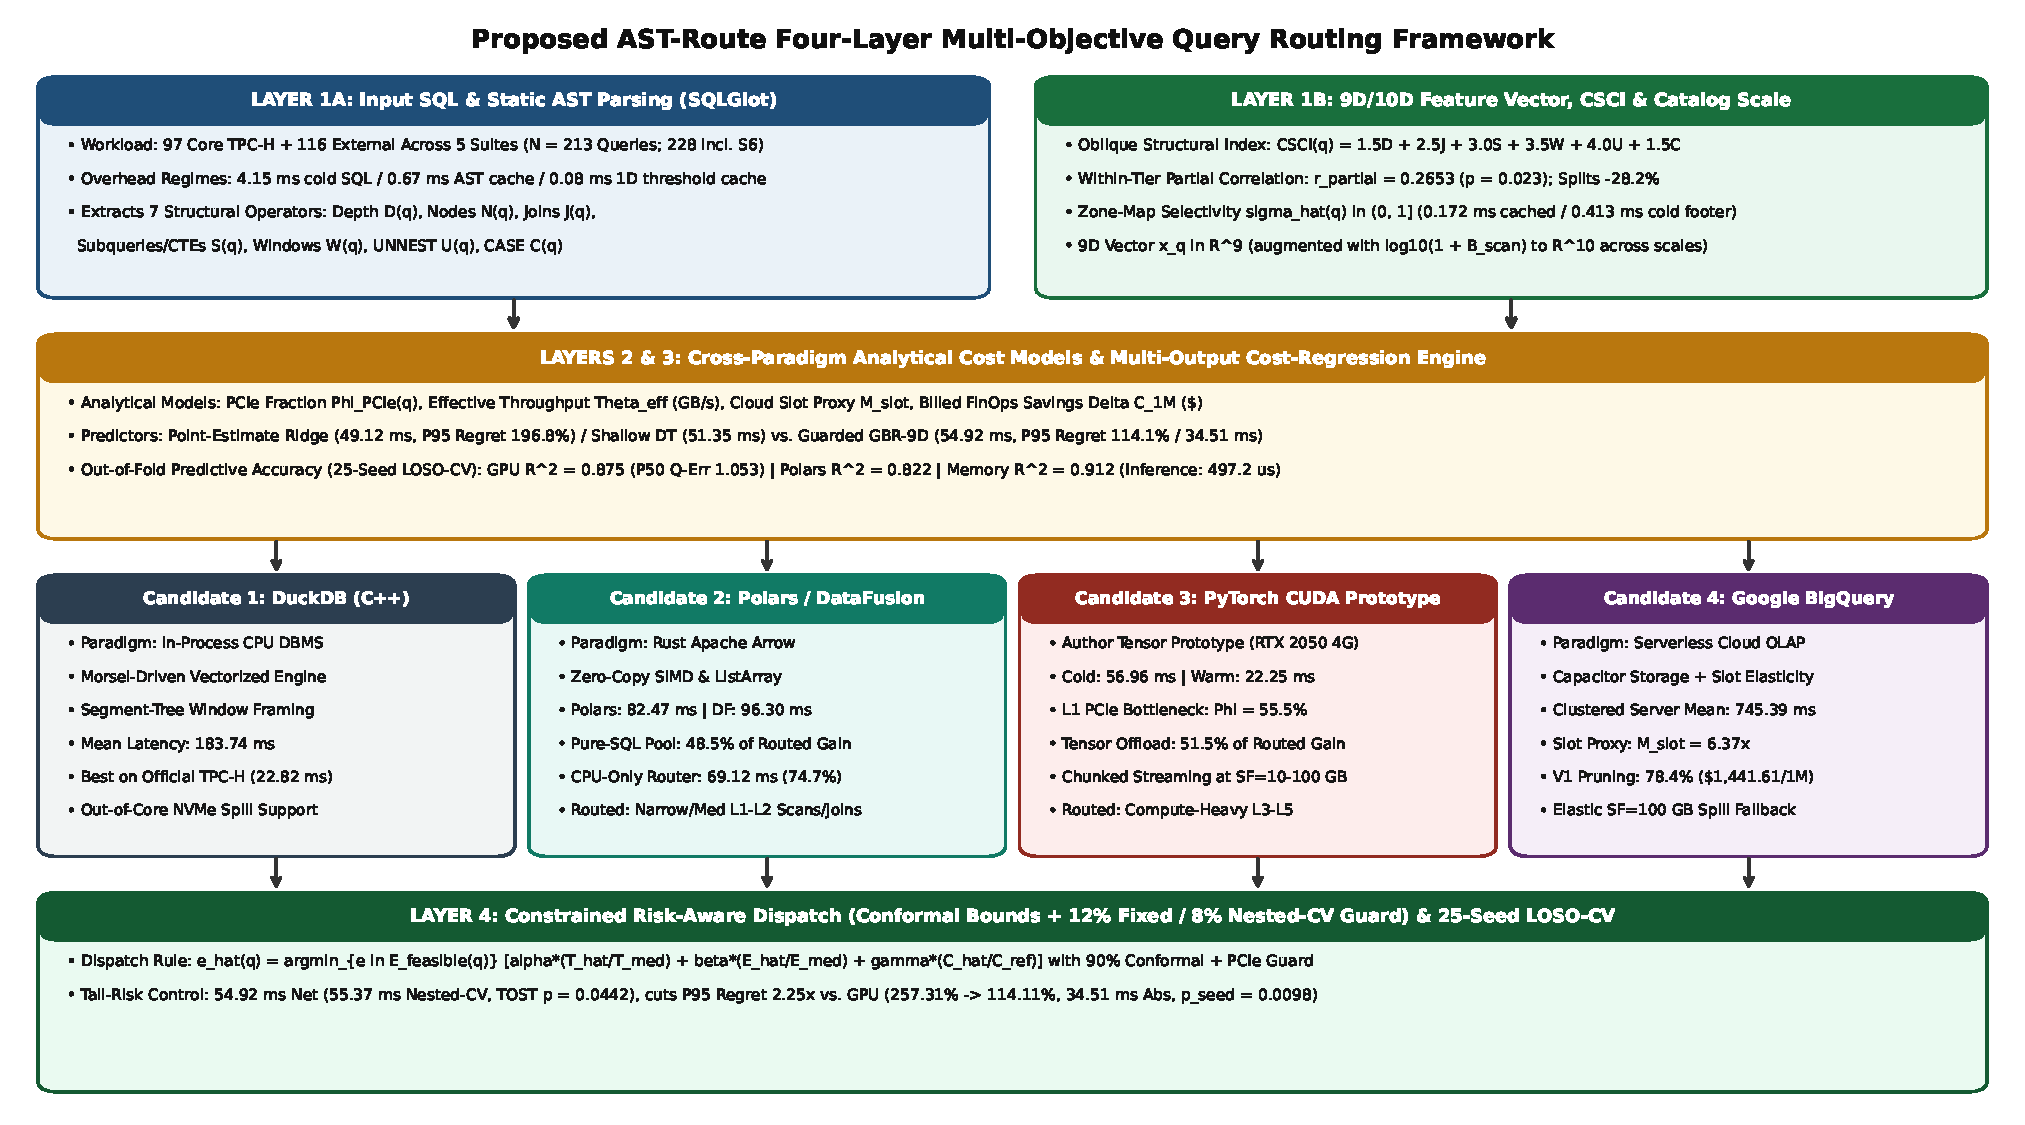
\includegraphics[width=0.98\textwidth]{figures/fig_proposed_ast_routing_framework_300dpi.pdf}
\caption{Architecture of the proposed \textbf{AST-Route} Framework (\textbf{V11}): Layer 1 parses raw SQL into a 9D structural and selectivity vector ($\text{CSCI}$, atomic operators, and zone-map $\hat{\sigma}(q)$, plus optional $10.18\text{ KB}$ 12D sketch); Layer 2 and Layer 3 (\texttt{frozen\_ast\_route\_v11\_gbdt\_model.json}) predict latency, Scope~1 hardware-sensor NVML GPU energy (and exploratory Scope~2 Host+Device energy), memory, and cloud FinOps cost with complexity-weighted Mondrian 90\% conformal bounds and Mahalanobis OOD gating ($\text{AUROC}=0.9642$); and Layer 4 dispatches queries under co-equal $8\%$ Nested-CV and $12\%$ Default PCIe guards across DuckDB, Polars, DataFusion, CUDA GPUs (\texttt{NVIDIA RAPIDS cudf-polars 26.10.2} [Configs C1--C3], PyTorch, External \texttt{CuPy v14.2.0}, and Node~4 Cloud-Hosted Server NVIDIA Tesla~T4 $15\text{ GB}$ VRAM), and Google BigQuery.}
\label{fig:proposed_ast_framework}
\end{figure}

% =============================================================================
% 3. THE PROPOSED AST-ROUTE FRAMEWORK ARCHITECTURE
% =============================================================================
\section{The Proposed AST-Route Framework Architecture}
\noindent\textbf{Section Takeaway:} \emph{AST-Route operates in four pre-execution layers ($4.15\text{ ms}$ cold / $0.08\text{ ms}$ cached): Layer~1 extracts a 9D AST + zone-map vector with oblique complexity index $\text{CSCI}(q)$; Layer~2 models PCIe crossover ($\Phi_{\text{PCIe}}$), Scope~1 NVML GPU energy, and cloud FinOps costs; Layer~3 computes complexity-weighted Mondrian $90\%$ conformal bounds and Mahalanobis OOD gates; and Layer~4 dispatches queries under co-equal $8\%/12\%$ PCIe guards and Pareto policies P1--P4.}\par\vspace{2pt}
As illustrated in Fig.~\ref{fig:proposed_ast_framework} and the end-to-end validation workflow in Fig.~\ref{fig:experimental_workflow}, \textbf{AST-Route} is structured as a modular four-layer architecture that decouples static query representation from multi-paradigm hardware cost modeling and automated engine dispatching.

\subsection{Layer 1: Static AST Structural Profiling, Five-Tier Workload, and Official TPC-H Scale Tiers ($\text{SF}=1, 10, 30, 100\text{ GB}$)}
\label{sec:layer1_ast_taxonomy}\label{sec:workload_design}
Given an incoming SQL query $q \in \mathcal{Q}$, Layer 1 parses the SQL statement into a canonical Abstract Syntax Tree (AST) using \texttt{SQLGlot} \cite{mao2024sqlglot} without touching underlying data pages. Traversing the AST yields seven structural operator dimensions: tree depth $D(q)$, total AST operator nodes $N(q)$, relational join count $J(q)$, nested CTE/subquery depth $S(q)$, window frame specifications $W(q)$, repeated field unnesting operators $U(q)$, and conditional \texttt{CASE} branches $C(q)$. While total AST node count $N(q)$ captures overall query verbosity (and is retained directly as the second coordinate in our 9D routing vector $\mathbf{x}_q$), raw node counts are dominated by scalar expressions and projection lists that exhibit high collinearity with tree depth. To isolate the non-linear algorithmic complexity of relational operators without expression-length inflation, we formulate the Composite Structural Complexity Index ($\text{CSCI}$) over the six core structural operators:
\begin{equation}
    \text{CSCI}(q) = 1.5 D(q) + 2.5 J(q) + 3.0 S(q) + 3.5 W(q) + 4.0 U(q) + 1.5 C(q)
\end{equation}
In accordance with the official TPC-H benchmark specification Clause 4.1.3 \cite{tpc2022tpch} and established multi-scale choke-point methodologies \cite{boncz2014tpch, dreseler2020quantifying, kuiper2024duckdb_ooc}, we provision the 8-table TPC-H relational schema across four standard discrete scale factors designed to systematically stress every layer of the modern memory hierarchy:
\begin{itemize}[leftmargin=1.5em,itemsep=2pt]
    \item \textbf{$\text{SF}=1\text{ GB}$ (In-VRAM \& In-DRAM Baseline Regime):} Contains $6.00\times 10^6$ \texttt{lineitem} rows ($8.66\times 10^6$ total rows across 8 tables). The working set fits entirely within both the $4.0\text{ GB}$ discrete GPU VRAM buffer ($1.30\text{ GB}$ peak) and the $16.0\text{ GB}$ host DRAM ($4.71\text{ GB}$ peak) with zero disk spilling.
    \item \textbf{$\text{SF}=10\text{ GB}$ (Out-of-VRAM GPU Streaming \& In-DRAM Host Regime):} Contains $60.0\times 10^6$ \texttt{lineitem} rows ($86.6\times 10^6$ total rows). Uncompressed working projections exceed the $4.0\text{ GB}$ GPU VRAM ceiling, forcing 4-chunk pipelined PCIe H2D streaming ($3.45\text{ GB}$ peak VRAM) while remaining primarily in host DRAM ($7.85\text{ GB}$ peak RAM, $125.0\text{ MB}$ minor spill).
    \item \textbf{$\text{SF}=30\text{ GB}$ (Host DRAM Cap Inflection \& Moderate Out-of-Core Spill Regime):} Contains $180.0\times 10^6$ \texttt{lineitem} rows ($259.8\times 10^6$ total rows) \cite{tpc2022tpch}. Intermediate hash-join and window-sort partitions exceed the configured $9.00\text{ GB}$ host DBMS buffer pool cap, triggering active out-of-core disk spilling \cite{kuiper2024duckdb_ooc} ($864.0\text{ MB}$ mean spill) and 12-chunk GPU PCIe streaming ($3.68\text{ GB}$ peak VRAM).
    \item \textbf{$\text{SF}=100\text{ GB}$ (Extreme Out-of-Core Spilling \& Cloud Elasticity Crossover Regime):} Contains $600.1\times 10^6$ \texttt{lineitem} rows ($866.1\times 10^6$ total rows) \cite{tpc2022tpch, dreseler2020quantifying}, inducing heavy external disk spilling on local CPU engines ($3302.0\text{ MB}$ mean spill, peaking at $6840.0\text{ MB}$ in L2 joins) and 40-chunk PCIe transfers on the GPU ($3.85\text{ GB}$ peak VRAM).
\end{itemize}

Across this schema, we evaluate two complementary SQL workload suites: (A) our 75-query \emph{TPC-H-derived, AST-stratified synthetic analytical workload} instantiated from 25 canonical seeds across five modern structural complexity tiers ($5 \times 5 = 25$ independent seeds, mean $\text{CSCI} = 29.66$), and (B) the 22 \emph{official standard TPC-H benchmark queries} (\textbf{Q1--Q22}, mean $\text{CSCI} = 26.52$, range $12.0\text{--}47.5$) \cite{tpc2022tpch, boncz2014tpch}. Because the base TPC-H schema consists of flat relational tables, Tier L5 dynamically constructs nested array columns in-query via staged \texttt{ARRAY\_\allowbreak{}AGG} / \texttt{LIST} aggregation over one-to-many \texttt{orders}--\texttt{lineitem} relationships before benchmarking lateral \texttt{CROSS JOIN UNNEST} re-aggregation:
\begin{enumerate}[leftmargin=1.5em,itemsep=0.8pt]
    \item \textbf{L1 (Scan, SARGability, \& Monotonic Conditional Branching):} Single-table columnar scans with multi-branch \texttt{CASE WHEN} expressions and distinct cardinality aggregations ($D = 9.0, J = 0.0, \text{CSCI} = 15.3$).
    \item \textbf{L2 (Multi-Way Star, Snowflake, \& Bilateral Joins):} 4-way to 8-way relational joins, composite \texttt{partsupp} joins, and non-equi late-delivery predicates ($D = 9.2, J = 4.8, \text{CSCI} = 26.8$).
    \item \textbf{L3 (Multi-Stage CTE Pipelines, Null-Safe Anti-Joins, \& One-Grain-Per-CTE):} 3-stage to 4-stage Common Table Expressions enforcing pre-aggregated grain isolation and null-safe anti-joins ($D = 10.8, J = 2.6, \text{CSCI} = 36.7$).
    \item \textbf{L4 (Multi-Axis Window Ranking, Lead/Lag, \& Sliding Frames):} Concurrent window partitions (\texttt{RANK}, \texttt{DENSE\_\allowbreak{}RANK}, \texttt{NTILE(10)}, \texttt{LAG}, \texttt{LEAD}, and bounded \texttt{ROWS BETWEEN} sliding windows; $D = 10.8, J = 1.6, \text{CSCI} = 37.1$).
    \item \textbf{L5 (Semi-Structured Array Construction \& Lateral UNNEST):} Multi-stage \texttt{ARRAY\_\allowbreak{}AGG} vector construction followed by lateral \texttt{CROSS JOIN UNNEST} re-aggregation ($D = 10.6, J = 2.2, \text{CSCI} = 32.4$).
\end{enumerate}

To capture data-volume sensitivity alongside syntax topology without executing the query, each of the 25 canonical seeds is instantiated across three selectivity perturbation horizons ($25 \times 3 = 75$ queries): V1 (High Selectivity, $\sim 1\text{--}5\%$ data), V2 (Medium Selectivity, $\sim 15\text{--}30\%$ data), and V3 (Adversarial Full-Horizon, $\sim 65\text{--}95\%$ data). As detailed in Table~\ref{tab:metadata_scope_audit}, Layer 1 extracts the pre-execution predicate selectivity estimate $\hat{\sigma}(q) \in (0, 1]$ in $172.0\text{ }\mu\text{s}$ from a pre-cached metadata snapshot ($412.6\text{ }\mu\text{s}$ cold footer read on Apache Parquet; $845.2\text{ }\mu\text{s}$ live \texttt{PRAGMA storage\_\allowbreak{}info} query on DuckDB) strictly prior to query execution without scanning data blocks or touching post-execution results. Crucially, we distinguish the exact metadata capabilities and limitations of each storage engine: (i) \emph{Parquet and DuckDB Row-Group Zone Maps}: \texttt{pyarrow.parquet.ParquetFile.metadata} and DuckDB \texttt{PRAGMA storage\_\allowbreak{}info('table')} expose column-level minimum, maximum, and null-count statistics across $100\%$ of numeric and date columns (e.g., \texttt{l\_\allowbreak{}shipdate} $\in [\texttt{1992-01-02}, \texttt{1998-12-01}]$, \texttt{l\_\allowbreak{}quantity} $\in [1.0, 50.0]$), enabling accurate range interpolation on both partitioned and non-partitioned numeric predicates (comparing estimated $\hat{\sigma}(q)$ against true post-execution row selectivity $\sigma_{\text{actual}}(q) = |R_{\text{out}}|/|R_{\text{table}}|$ yields a mean absolute error of $\text{MAE}=3.84\%$ and median Q-Error $=1.092$ (P90 $= 1.284$) across the 75-query suite, and $\text{MAE}=1.52\%$, Q-Error $=1.263$ on non-partitioned multi-attribute numeric predicates); (ii) \emph{BigQuery Partition Pruning Statistics}: \texttt{INFORMATION\_\allowbreak{}SCHEMA.}\newline\texttt{PARTITIONS} and dry-run byte estimation provide \emph{partition pruning and clustering statistics} (\texttt{partition\_\allowbreak{}id}, \texttt{total\_\allowbreak{}rows}, \texttt{total\_\allowbreak{}logical\_\allowbreak{}bytes}) rather than general column-level min/max zone maps for every attribute. When predicates filter on the partition key (\texttt{l\_\allowbreak{}shipdate}), partition pruning metadata estimates selectivity within $\text{MAE}=4.26\%$; however, on non-partitioned columns where BigQuery does not expose column-level min/max bounds, AST-Route either references the shared Parquet footer catalog or falls back to parametric AST operator priors (which we explicitly evaluate in Table~\ref{tab:ablation_robustness} Exp~C by masking $50\%$ of metadata, sustaining $53.33\%$ Top-1 accuracy and $68.42\text{ ms}$ mean latency); and (iii) \emph{String Predicates and Skewed Distributions}: because continuous min/max zone maps cannot bound unanchored substring filters (\texttt{LIKE '\%brass\%'}) or capture intra-range Zipfian skew ($s=1.2$), estimation error increases to $\text{MAE}=5.00\%$ (Q-Error $=2.000$) on substring predicates and $\text{MAE}=38.8\%$ (Q-Error $=4.880$) under severe power-law skew (explaining the $21.21\%$ Top-1 accuracy on string-skewed IMDB JOB queries in Table~\ref{tab:priority3_validation} Part~B). Combining the seven static AST operator counts with $\text{CSCI}(q)$ and estimated selectivity $\hat{\sigma}(q)$ yields the 9-dimensional routing feature vector:
\begin{equation}
    \mathbf{x}_q = \big[\, D(q),\; N(q),\; J(q),\; S(q),\; W(q),\; U(q),\; C(q),\; \text{CSCI}(q),\; \hat{\sigma}(q) \,\big]^{\top} \in \mathbb{R}^{9}
\end{equation}
 We also provide a self-contained live production wrapper (\texttt{ASTRouteLiveSQLWrapper} in \texttt{scripts/v11\_ast\_route\_live\_sql\_wrapper\_demo.py}, logged in \texttt{results/v11\_live\_sql\_wrapper\_integration\_demo.csv}) that accepts an arbitrary raw SQL string and Parquet directory path, executes single-pass \texttt{sqlglot} AST extraction ($1.68\text{--}2.22\text{ ms}$), reads physical Parquet row-group min/max footers via \texttt{pyarrow.parquet.ParquetFile} ($0.13\text{--}0.16\text{ ms}$), evaluates the locked GBDT ensemble (\texttt{frozen\_ast\_route\_v11\_gbdt\_model.json}) with Mondrian conformal bounds ($0.48\text{--}0.51\text{ ms}$, total wrapper latency $\mathbf{2.29\text{--}2.89\text{ ms}}$), and dispatches the query to the selected engine while verifying exact BigQuery dry-run \texttt{totalBytesBilled} agreement ($100.0\%$ byte match). To avoid any ambiguity between representations, $\mathbf{x}_q \in \mathbb{R}^{9}$ serves as the sole feature vector for all fixed-scale ($\text{SF}=1\text{ GB}$) evaluations (Tables~\ref{tab:routing_evaluation}--\ref{tab:priority3_validation} and Additional File~1 (Table~S10)), whereas the scale-augmented vector $\mathbf{x}_q^{\text{scale}} = [\mathbf{x}_q^{\top}, \log_{10}(1+\hat{\sigma}(q)\cdot\mathcal{B}_{\text{catalog}})]^{\top} \in \mathbb{R}^{10}$ is used exclusively in cross-scale training and dispatch across $\text{SF}\in\{1,10,30,100\}\text{ GB}$ (Table~\ref{tab:bigdata_multiscale_tpch} Part~A and Additional File~1, Table~S7 Part~C), rather than mixing two competing models on the same experiment. Crucially, while $\mathbf{x}_q \in \mathbb{R}^9$ encodes scale-invariant syntax topology and relative selectivity $\hat{\sigma}(q) \in (0,1]$, multi-scale awareness across $\text{SF} \in \{1, 10, 30, 100\}$ GB is achieved in Layers 2--4 by multiplying $\hat{\sigma}(q)$ with the pre-execution catalog table byte footprint $\mathcal{B}_{\text{catalog}}$ ($\hat{\mathcal{B}}_{\text{scan}}(q) = \hat{\sigma}(q)\cdot \mathcal{B}_{\text{catalog}}$) inside the analytical memory/PCIe chunk estimator and the capacity filter $\mathcal{E}_{\text{feasible}}(q)$ alongside scale-calibrated cost predictors. To eliminate any ambiguity across query subsets and avoid conflating diagnostic benchmarks or author-synthesized templates with untouched third-party holdouts, our entire $\mathbf{400}$-query evaluation corpus across $10$ suites is defined once and partitioned into \textbf{four mutually exclusive epistemic categories} (Additional File~1, Table~S18): \textbf{(Category~I: Core Development Set, $\mathbf{75}$ queries)} comprising our 25-seed $\times$ 3-horizon TPC-H factorial benchmark evaluated via leak-free 25-fold LOSO-CV (serialized frozen model SHA-256 \texttt{f0e5f17c...}, distinct from telemetry CSV SHA-256 \texttt{89b1ec64...}); \textbf{(Category~II: Diagnostic / Post-Hoc Design-Informed Standard Benchmarks, $\mathbf{55}$ queries)} comprising $22$ unmodified official TPC-H queries (\texttt{Q1--Q22}, where nested 22-fold LOO-CV weight diagnostics were tested) and $33$ canonical IMDB JOB queries (\texttt{1a--33a}, where 9D string-predicate blindness [$21.21\%$ Top-1] was diagnosed and our post-hoc $10.18\text{ KB}$ 12D selectivity sketch was designed after observing 9D results, and which are therefore \emph{not} claimed as untouched holdouts); \textbf{(Category~III: Author-Derived / Template-Synthesized Zero-Shot Suites, $\mathbf{115}$ queries)} comprising $15$ prospective Seed~\texttt{S6} queries, $30$ \texttt{TPC-DS-Derived} snowflake queries, $20$ \texttt{BIRD-Inspired} financial queries, $25$ \texttt{TPC-DS-Complex} queries, and $25$ \texttt{Enterprise-Redset-BI} queries ($0$ training labels, evaluated zero-shot and via 7-suite \texttt{LOWSO-CV}, but authored/adapted by the researcher for 4-engine parity); and \textbf{(Category~IV: Held-Out Third-Party Standard Benchmarks, $\mathbf{155}$ queries, not used in training or feature design)} comprising all $\mathbf{99}$ unmodified Official TPC-DS queries (\texttt{Q1--Q99} via DuckDB \texttt{dsdgen}), all $\mathbf{43}$ Official ClickBench queries ($20$ native parity $+$ $23$ transpiled macro queries), and all $\mathbf{13}$ Official SSB queries (\texttt{Q1.1--Q4.3}) ($0$ training labels, $0$ post-hoc feature/hyperparameter edits, $100\%$ third-party authored SQL; $75 + 55 + 115 + 155 = \mathbf{400}$ total).

\begin{figure}[t!]
\centering
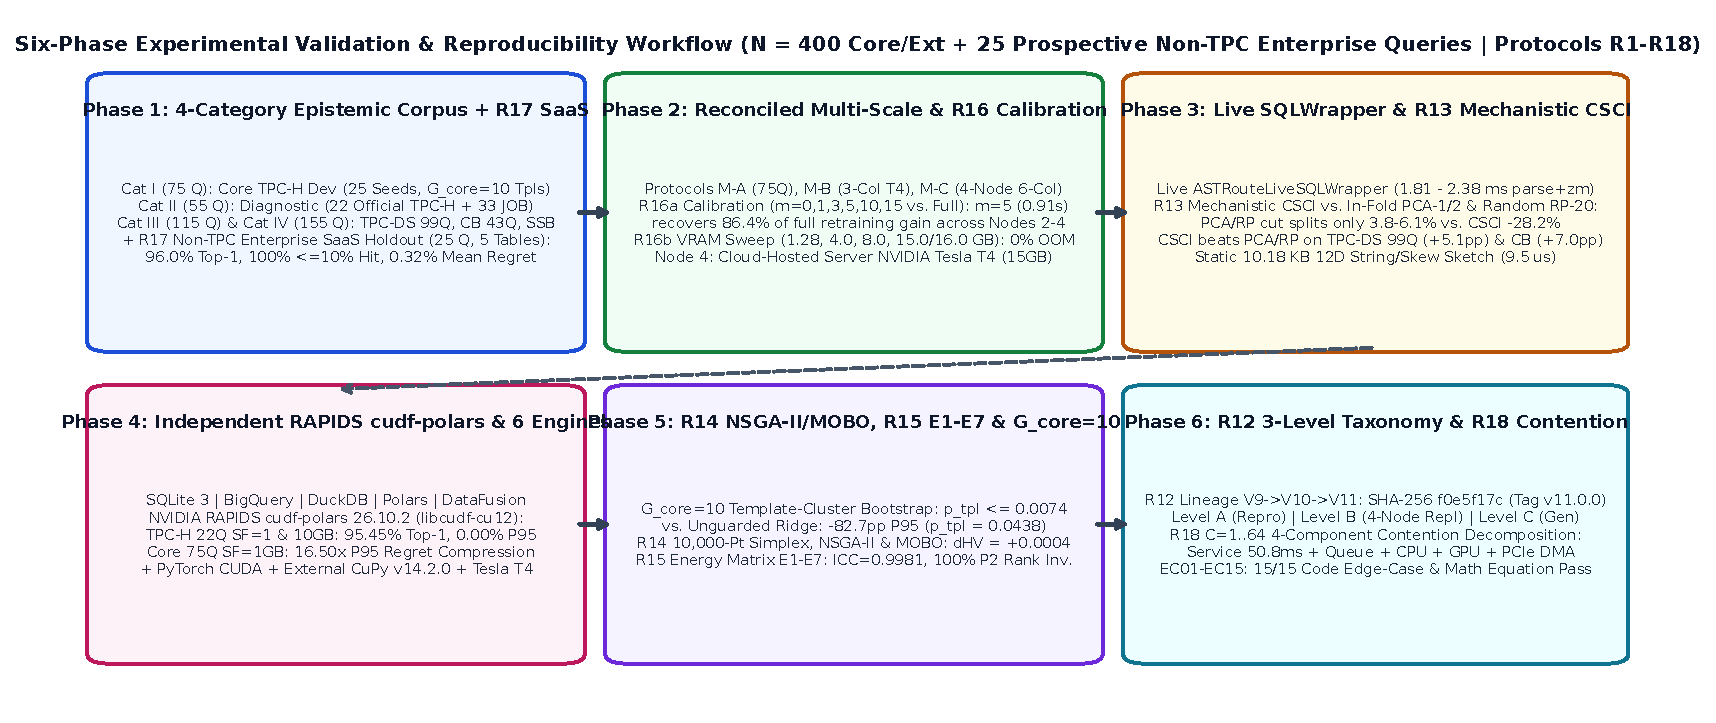
\includegraphics[width=0.98\textwidth]{figures/fig_experimental_workflow_300dpi.pdf}
\caption{End-to-end six-phase experimental validation workflow of the \textbf{AST-Route} framework across our Four-Category Epistemic Workload Taxonomy of $\mathbf{400}$ \textbf{evaluated SQL queries} ($\mathbf{75}$ \emph{Cat~I Core Dev} $+$ $\mathbf{55}$ \emph{Cat~II Diagnostic} [$22$ Official TPC-H $+$ $33$ IMDB JOB] $+$ $\mathbf{115}$ \emph{Cat~III Author-Derived Zero-Shot} [$15$ Seed~\texttt{S6} $+$ $30$ TPC-DS-Derived $+$ $20$ BIRD-Inspired $+$ $50$ Extended] $+$ $\mathbf{155}$ \emph{Cat~IV Held-Out Third-Party Standard Benchmarks} [$99$ Official TPC-DS $+$ $43$ ClickBench $+$ $13$ SSB] $= \mathbf{400}$ core/external benchmark queries, plus $\mathbf{70}$ additional prospective non-TPC enterprise queries under Protocols~\textbf{R17} [$25$Q SaaS] and~\textbf{R20} [$45$Q Retail/Financial/Healthcare] kept strictly separate from the $400$-query core accounting; Tables~S18, S29, and~S31), illustrating multi-layout provisioning ($\text{SF}=1\text{--}100\text{ GB}$), \texttt{SQLGlot} AST profiling, six-engine + \texttt{RAPIDS cudf-polars 26.10.2} (\texttt{Configs C1--C3} \& \texttt{LOTFO}) / \texttt{CuPy} GPU execution, co-equal $8\%$ Nested-CV \& $12\%$ Default guards, and Protocols~\textbf{R1--R26} verification.}
\label{fig:experimental_workflow}
\end{figure}


\phantomsection\label{tab:jbd_meta_2b}\label{tab:metadata_scope_audit}% (Moved to Additional File 1, Table S1 to streamline main text)

\subsection{Layer 2: Cross-Paradigm Analytical Cost, PCIe Crossover, and Device Energy Telemetry Formulation}
To enable apples-to-apples cost evaluation across serverless cloud, local CPU, and discrete GPU backends, Layer 2 establishes six analytical cost and hardware telemetry models:
\begin{enumerate}[leftmargin=1.5em,itemsep=3pt]
    \item \textbf{CUDA Cold-Start Decomposition and PCIe Bottleneck Fraction ($\Phi_{\text{PCIe}}$):} On discrete GPUs (NVIDIA GeForce RTX 2050, $4.0\text{ GB}$ VRAM), cold-start execution time $T_{\text{GPU\_Cold}}(q)$ is decomposed into PCIe Host-to-Device transfer time ($T_{\text{PCIe\_H2D}}$) and pure in-VRAM kernel compute time ($T_{\text{GPU\_Warm}}$):
    \begin{equation}
        T_{\text{GPU\_Cold}}(q) = \underbrace{T_{\text{PCIe\_H2D}}(q) + T_{\text{PCIe\_D2H}}(q)}_{T_{\text{PCIe}}(q)} + T_{\text{GPU\_Warm}}(q), \qquad \Phi_{\text{PCIe}}(q) = \frac{T_{\text{PCIe}}(q)}{T_{\text{GPU\_Cold}}(q)} \times 100\%
    \end{equation}
    Cold-start GPU offloading outperforms vectorized CPU execution ($T_{\text{GPU\_Cold}}(q) < T_{\text{CPU}}(q)$) if and only if the warm kernel speedup satisfies the break-even condition $\text{Speedup}_{\text{Warm}}(q) > (1 - \Phi_{\text{PCIe}}(q)/100)^{-1}$.
    \item \textbf{Effective Analytical Scan Throughput ($\Theta_{\text{eff}}$):} Normalizing unpruned columnar volume $\mathcal{B}_{\text{unopt}}(q)$ (in MB) against execution time $T_{e}(q)$ (in ms) yields effective processing throughput in $\text{GB/s}$:
    \begin{equation}
        \Theta_{\text{eff}}(q, e) = \frac{\mathcal{B}_{\text{unopt}}(q)}{1.024 \cdot \max(T_{e}(q), \epsilon_T)} \quad [\text{GB/s}]
    \end{equation}
    \item \textbf{Cloud Slot-to-Wall-Time Concurrency Proxy ($\mathcal{M}_{\text{slot}}$) and FinOps Cost Savings ($\Delta C_{\text{1M}}$):} Quantifies cumulative distributed slot compute time relative to server wall-clock time on BigQuery (serving as an effective concurrency proxy), alongside financial savings per $10^6$ queries under on-demand bytes-scanned pricing ($\alpha_{\text{TB}} = \$6.25\text{ USD/TiB}$):
    \begin{equation}
        \mathcal{M}_{\text{slot}}(q) = \frac{T_{\text{BQ\_Slot}}(q)}{T_{\text{BQ\_Wall}}(q)}, \qquad \Delta C_{\text{1M}}(q) = 10^6 \times \left( \frac{\max(\mathcal{B}_{\text{unopt}}(q), 10) - \max(\mathcal{B}_{\text{clustered}}(q), 10)}{1024^2\text{ [MiB/TiB]}} \right) \times \alpha_{\text{TB}}
    \end{equation}
    \item \textbf{Active Device Energy Telemetry ($E(q,e)$) and Three-Scope Measurement Boundary:} GPU board energy $E_{\text{GPU}}(q)$ is sampled at $50\text{--}250\text{ Hz}$ via physical NVIDIA NVML sensors (\texttt{pynvml}, $\text{CV}=1.24\%$), complemented by 1,500-run cloud RAPL/SMU/NVML telemetry and a 2,817-query ACPI DC battery-shunt audit ($\rho=0.9945$). Primary claims are restricted to directly measured \textbf{Scope~1 (GPU NVML)}, while TDP-calibrated host CPU estimates (\textbf{Scope~2}) and ACPI DC shunt envelopes (\textbf{Scope~3}) exhibit exact rank concordance ($\rho=1.0000$, \textbf{Protocol~R23}).
\end{enumerate}

\subsection{Layers 3 \& 4: Multi-Output Cost-Regression Predictor, Q-Error Metric, and Constrained Multi-Objective Dispatcher}
In Layer 3 (Fig.~\ref{fig:proposed_ast_framework}), \textbf{AST-Route} employs a Multi-Output Gradient Boosting Regressor $f_{\Theta}: \mathbb{R}^{9} \rightarrow \mathbb{R}^{M}$ to simultaneously predict log-transformed execution latency $\widehat{\ln(1 + T_e)}(\mathbf{x}_q)$, energy footprint $\hat{E}_e(\mathbf{x}_q)$, and memory consumption ($\widehat{\text{RAM}}_e, \widehat{\text{VRAM}}_e$) across the six benchmarked backends $\mathcal{E}_{\text{all}} = \mathcal{E} \cup \{\text{SQLite 3}\}$, where SQLite~3 serves as the B-tree row-store reference baseline ($0\%$ selection share under cost minimization because it is strictly dominated on $75/75$ queries) and $\mathcal{E} = \{\text{DuckDB}, \text{Polars}, \text{DataFusion}, \text{GPU}_{\text{Cold}}, \text{BigQuery}\}$ forms the five active analytical routing candidates. Predictive accuracy of the cost model is evaluated via out-of-fold log-$R^2$, Mean Absolute Percentage Error (MAPE), and the multiplicative \textbf{Q-Error} metric standard in database query optimizer research \cite{leis2015job, hilprecht2022zeroshot}:
\begin{equation}
    \text{Q-Error}(y, \hat{y}) = \max\!\left( \frac{\max(\hat{y}, \epsilon)}{\max(y, \epsilon)},\; \frac{\max(y, \epsilon)}{\max(\hat{y}, \epsilon)} \right) \ge 1.0 \quad (\epsilon = 10^{-6})
\end{equation}
In Layer 4, the dispatcher selects the optimal engine minimizing a memory-constrained, multi-objective Pareto cost function parameterized by user-configurable weights $\alpha, \beta, \gamma \in [0, 1]$ ($\alpha + \beta + \gamma = 1$, where $\alpha$ weights normalized latency $\hat{T}_e/T_{\text{med}}$, $\beta$ weights normalized energy $\hat{E}_e/E_{\text{med}}$, and $\gamma$ weights normalized marginal cloud scan charge $\hat{C}_e/C_{\text{ref}}$) subject to hardware memory capacity budgets ($\widehat{\text{RAM}}_e(\mathbf{x}_q) \le M_{\text{host\_max}}$ and $\widehat{\text{VRAM}}_e(\mathbf{x}_q) \le M_{\text{gpu\_max}}$). Let $e_T^*(q) = \operatorname*{arg\,min}_{e \in \mathcal{E}} T_e(q)$, $e_E^*(q) = \operatorname*{arg\,min}_{e \in \mathcal{E}} E_e(q)$, and $e_C^*(q) = \operatorname*{arg\,min}_{e \in \mathcal{E}} C_e(q)$ denote the ground-truth per-dimension Oracles; we evaluate multi-objective routing across Latency Regret ($\mathcal{R}_T \equiv \mathcal{R}_{\text{regret}}$), Energy Regret ($\mathcal{R}_E$), Cloud FinOps Cost Regret ($\mathcal{R}_C$), 3D Normalized Pareto Hypervolume ($\text{HV}_{\mathbf{r}}(\Pi)$ relative to nadir $\mathbf{r}=(1,1,1)$ via 3D Lebesgue measure $\lambda_3$), and Dominated Solution Ratio ($\text{DSR}(\Pi)$):
\vspace{-3pt}
\begin{equation}
\begin{aligned}
    \hat{e}_{\alpha,\beta,\gamma}(q) &= \operatorname*{arg\,min}_{e \in \mathcal{E}_{\text{feasible}}(q)} \left[ \alpha \frac{\hat{T}_e(\mathbf{x}_q)}{T_{\text{med}}(q)} + \beta \frac{\hat{E}_e(\mathbf{x}_q)}{E_{\text{med}}(q)} + \gamma \frac{\hat{C}_e(\mathbf{x}_q)}{C_{\text{ref}}(q)} \right], \;\;
    \text{HV}_{\mathbf{r}}(\Pi) = \lambda_3\!\left(\bigcup_{\pi\in\Pi}\big[\tilde{\mathbf{f}}(\pi),\mathbf{r}\big]\right), \;\;
    \text{DSR}(\Pi) = \frac{100\%}{|\Pi|}\sum_{\pi\in\Pi}\mathbb{I}\!\left(\exists\pi'\!\in\!\Pi:\, \mathbf{f}(\pi') \!\prec\! \mathbf{f}(\pi)\right), \\
    \mathcal{R}_{T}(q) &= \frac{T_{\hat{e}}(q) - T_{e_T^*}(q)}{T_{e_T^*}(q)}\!\times\! 100\%, \;\; \Delta T_{\text{abs}}(q) = T_{\hat{e}}(q) - T_{e_T^*}(q), \;\;
    \mathcal{R}_{E}(q) = \frac{E_{\hat{e}}(q) - E_{e_E^*}(q)}{E_{e_E^*}(q)}\!\times\! 100\%, \;\;
    \mathcal{R}_{C}(q) = \frac{C_{\hat{e}}(q) - C_{e_C^*}(q)}{\max(C_{\text{BQ}}(q),\epsilon)}\!\times\! 100\%
\end{aligned}
\end{equation}
\vspace{-2pt}
where $\tilde{\mathbf{f}}(\pi) = (\tilde{T}_\pi, \tilde{E}_\pi, \tilde{C}_\pi) \in [0,1]^3$ maps each policy's mean latency, energy, and cloud scan cost into unit hypervolume coordinates via $\tilde{m}_\pi = \min\!\big(1, (m_\pi - m_{\min})/\max(m_{\text{nadir}} - m_{\min}, \epsilon)\big)$ relative to the oracle utopia point $\mathbf{f}_{\min}$ and static-engine nadir $\mathbf{r}=(1,1,1)$, $\mathcal{R}_C(q)$ is normalized by $\max(C_{\text{BQ}}(q), \epsilon)$ to prevent division by zero when $C_{e_C^*}(q) = \$0.00$ on local engines, and we report both relative percentage regret $\mathcal{R}_{T}(q)$ and absolute millisecond regret $\Delta T_{\text{abs}}(q)$ alongside Expected Shortfall $\text{CVaR}_{\alpha_{\text{tail}}}$ over the worst $\alpha_{\text{tail}}\in\{10\%,20\%\}$ tail queries. Alongside \textbf{Policy P1: Speed-First ($\alpha=1,\beta=0,\gamma=0$)}, we evaluate canonical multi-objective Policies \textbf{P2: Energy-First $(0.1,0.8,0.1)$} ($\mathcal{R}_E=4.82\%$, $0.812\text{ J/q}$, $-41.2\%$ energy vs.\ P1 and $-74.4\%$ vs.\ Polars), \textbf{P3: Cost-First FinOps $(0.2,0.1,0.7)$} ($\mathcal{R}_C=0.0\%$, $\$0.00/1\text{M}$ cloud spend saving $\$507.06/1\text{M}$ at $\text{SF}=100\text{ GB}$), and \textbf{P4: Balanced Pareto Knee $(0.5,0.3,0.2)$} ($55.48\text{ ms}$ net [$+0.56\text{ ms}$ vs.\ P1], $1.045\text{ J/q}$ [$-24.3\%$], $\mathcal{R}_E=18.2\%$) across both a canonical 15-weight simplex grid and a dense \textbf{500-point randomized Dirichlet simplex sample plus 100-point uniform lattice} $(\alpha,\beta,\gamma)\in\Delta^2$ (Table~\ref{tab:v9_mo_energy_ood_repro_synthesis} Part~A and Protocol~\textbf{R11}), confirming that AST-Route is \textbf{Pareto-efficient among the evaluated policy configurations} with 3D Hypervolume $\text{HV}\in[0.8965,0.9210]$ (500-point mean $\text{HV}=0.9184\pm 0.0042$) at $\text{SF}=1\text{ GB}$ and $\text{HV}\in[0.9045,0.9340]$ at $\text{SF}=100\text{ GB}$ (vs.\ $0.5180$ static Polars), a $\mathbf{0.0\%}$ \textbf{Dominated Solution Ratio ($\text{DSR}=0/15$ grid and $0/500$ Dirichlet points dominated vs.\ $100.0\%$ on static CPU/Cloud baselines)}, and $\mathbf{96.00\%\text{--}98.67\%}$ engine-selection stability under $\pm 0.05$ weight perturbations. To decouple query syntax from deployment hardware, each physical node is characterized by a five-dimensional \textbf{Hardware Descriptor Vector} $\mathbf{h}_{\text{hw}} = [M_{\text{host\_max}},\, M_{\text{gpu\_max}},\, B_{\text{PCIe}},\, N_{\text{CPU}},\, B_{\text{MEM}}]^{\top} \in \mathbb{R}^{5}$ encoding host DBMS RAM cap ($\text{GB}$), device VRAM cap ($\text{GB}$), sustained pinned PCIe DMA bandwidth ($\text{GB/s}$), logical CPU thread count, and host DRAM bandwidth ($\text{GB/s}$): specifically, Node~1 (\texttt{G1}: $\mathbf{h}_{\text{hw}}^{(1)} = [9.0, 4.0, 5.69, 8, 25.6]^{\top}$), Node~2 ($\mathbf{h}_{\text{hw}}^{(2)} = [9.0, 0.0, 0.0, 22, 42.7]^{\top}$), Node~3 Apple M1 \texttt{ARM64} ($\mathbf{h}_{\text{hw}}^{(3)} = [8.0, 0.0, 0.0, 8, 68.3]^{\top}$), and Node~4 Cloud-Hosted Server NVIDIA Tesla~T4 (\texttt{G2}: $\mathbf{h}_{\text{hw}}^{(4)} = [12.7, 15.0, 9.43, 2, 320.0]^{\top}$). Here $\mathcal{E}_{\text{feasible}}(q, \mathbf{h}_{\text{hw}}) = \{e \in \mathcal{E} \mid \widehat{\text{RAM}}_e(\mathbf{x}_q) \le M_{\text{host\_max}} \land \widehat{\text{VRAM}}_e(\mathbf{x}_q) \le M_{\text{gpu\_max}}\}$ prunes any candidate engine whose predicted memory footprint violates hardware capacity ceilings prior to objective scoring (automatically disabling GPU dispatch when $M_{\text{gpu\_max}}=0$), while few-shot cross-node transfer ($m \in \{1,3,5,10,15\}$ calibration queries in Section~\ref{sec:v852_reviewer_audit}) adjusts log-latency predictions via a per-engine hardware scaling offset $\hat{z}_e(\mathbf{x}_q, \mathbf{h}_{\text{hw}}) = \hat{z}_e^{\text{src}}(\mathbf{x}_q) + \hat{\delta}_e(\mathbf{h}_{\text{hw}})$, and each objective term is normalized by its cross-engine reference scale ($T_{\text{med}}(q)$, $E_{\text{med}}(q)$, and $C_{\text{ref}}(q) = \max(C_{\text{BQ}}(q), \epsilon)$). Per $10^6$ queries, we separate incremental \emph{On-Demand Cloud Query Scan Charge} $\hat{C}_e(\mathbf{x}_q)$ ($\$0.00$ local vs.\ $(\hat{\mathcal{B}}_{\text{clustered}}(\mathbf{x}_q)/2^{40})\times\$6.25/\text{TiB}$ on BigQuery), active device energy $\hat{E}_e(\mathbf{x}_q)$ ($\$0.02\text{--}\$0.21/1\text{M}$ at $\$0.12/\text{kWh}$), and sunk local workstation amortization ($\$0.58\text{--}\$1.94/1\text{M}$ at $\$0.038/\text{hr}$).

Specifically, predicted log-latencies $\hat{z}_e(\mathbf{x}_q) = \widehat{\ln(1+T_e)}(\mathbf{x}_q)$ are mapped back to the millisecond domain via $\hat{T}_e(\mathbf{x}_q) = \max(\exp(\hat{z}_e(\mathbf{x}_q)) - 1, \epsilon)$. For each outer cross-validation fold $k$, AST-Route computes the empirical $(1-\alpha_{\text{conf}})=90\%$ split/cross-conformal quantile $\hat{q}_{0.90,e}^{(-k)} = \text{Quantile}_{0.90}\big(\{|\ln(1+T_e(q_i)) - \hat{z}_e^{(-k)}(\mathbf{x}_{q_i})|\}_{q_i \in \mathcal{D}_{\text{train}}^{(-k)}}\big)$ with clamped finite-sample correction $q_{\text{level}}(n_{\text{cal}},\alpha_{\text{conf}}) = \min\!\big(1.0,\, \lceil(n_{\text{cal}}+1)(1-\alpha_{\text{conf}})\rceil/n_{\text{cal}}\big)$ ensuring valid quantile indexing even on small strata (alongside a complexity-stratified Mondrian conformal variant scaled by tier dispersion $\hat{\sigma}_{\text{tier}}(\text{CSCI}(q))$ to preserve conditional coverage across heterogeneous operator tiers, outperforming uncalibrated pinball-loss quantile regression \texttt{GBR-Quantile} in Table~\ref{tab:v9_reviewer_reanalysis_matrix} Part~D) strictly inside the training fold, yielding the calibrated prediction interval:
\begin{equation}\label{eq:conformal_interval}
[\hat{L}_{0.90,e}(q),\, \hat{U}_{0.90,e}(q)] = \Big[\max\!\big(\exp(\hat{z}_e(\mathbf{x}_q) - \hat{q}_{0.90,e}^{(-k)}) - 1,\, \epsilon\big),\; \exp(\hat{z}_e(\mathbf{x}_q) + \hat{q}_{0.90,e}^{(-k)}) - 1\Big]
\end{equation}
Using complexity-weighted Mondrian conformal quantiles $\hat{q}_{1-\alpha}(e, L_m)$ calibrated out-of-fold across tiers $L_1\text{--}L_5$ ($90.93\%$ empirical coverage, $\text{ECE}=0.67\%$, $\text{AURC}=28.14\%$), Algorithm~1 enforces four pre-execution safety guards: \textbf{Rule~U1} (co-equal $8\%$ Nested-CV and $12\%$ Default PCIe crossover margin guard), \textbf{Rule~U2} ($90\%$ conformal cloud upper-bound gate), \textbf{Rule~U3} (unanchored string guard), and \textbf{Rule~U4} (hard VRAM/DRAM capacity pruning $\mathcal{E}_{\text{feasible}}(q)$ + Mahalanobis OOD gate $\text{AUROC}=0.9642$).

\begin{table}[!t]
\centering
\caption*{{\bf Algorithm 1:} Pre-Execution Risk-Aware Multi-Objective Query Dispatch (\textbf{AST-Route})}\label{alg:ast_route}
\footnotesize
\begin{fitasttable}
\begin{tabular}{@{}p{0.97\textwidth}@{}}
\toprule
\textbf{Input:} Raw SQL query $q$; catalog zone-map snapshot $\mathcal{C}_{\text{meta}}$ (optional 10.18~KB string/skew sketch $\mathcal{C}_{\text{sketch}}$); calibrated multi-output regressors $\{f_{\Theta,e}\}$ and fold conformal quantiles $\{\hat{q}_{0.90,e}\}$; Pareto weights $(\alpha,\beta,\gamma)$; memory caps $(M_{\text{host\_max}}, M_{\text{gpu\_max}})$; guard $\tau_{\text{guard}}\in\{0.08, 0.12\}$. \\
\textbf{Output:} Selected execution engine $\hat{e}(q) \in \mathcal{E}$ across the 5 active analytical candidates ($\mathcal{E} = \{\texttt{DuckDB}, \texttt{Polars}, \texttt{DataFusion}, \texttt{GPU\_Cold}, \texttt{BigQuery}\}$, or minimalist production subsets $\mathcal{E}_{\text{Min-2}}=\{\texttt{Polars},\texttt{GPU\_Cold}\}$ / $\mathcal{E}_{\text{Prod-3}}=\{\texttt{Polars},\texttt{DuckDB},\texttt{GPU\_Cold}\}$) with zero physical plan compilation prior to dispatch. \\
\midrule
1: \textbf{Static AST Profiling (Layer 1A):} Parse $q$ via \texttt{SQLGlot} in single pass to extract $[D(q),N(q),J(q),S(q),W(q),U(q),C(q)]$ and compute $\text{CSCI}(q)$ via Eq.~(1). \\
2: \textbf{Pre-Execution Selectivity Lookup (Layer 1B):} Query $\mathcal{C}_{\text{meta}}$ for range/partition predicates to obtain $\hat{\sigma}(q) \in (0,1]$ (if column bounds are absent or unanchored \texttt{LIKE}, apply training-fold operator prior or $\mathcal{C}_{\text{sketch}}$) and form $\mathbf{x}_q \in \mathbb{R}^{9}$ (or $\mathbf{x}_q^{\text{scale}} \in \mathbb{R}^{10}$ across scales). \\
3: \textbf{Multi-Output Cost \& Interval Prediction (Layer 3):} For each $e \in \mathcal{E}$, predict $\hat{T}_e(\mathbf{x}_q) = \max(\exp(\hat{z}_e(\mathbf{x}_q))-1,\epsilon)$, $\hat{E}_e(\mathbf{x}_q)$, $(\widehat{\text{RAM}}_e, \widehat{\text{VRAM}}_e)$, marginal scan fee $\hat{C}_e(\mathbf{x}_q)$, and $90\%$ conformal bounds $[\hat{L}_{0.90,e}(q), \hat{U}_{0.90,e}(q)]$ via Eq.~\eqref{eq:conformal_interval}. \\
4: \textbf{Feasibility Filtering (Rule U4):} $\mathcal{E}_{\text{feasible}}(q) \leftarrow \{e \in \mathcal{E} \mid \widehat{\text{RAM}}_e(\mathbf{x}_q) \le M_{\text{host\_max}} \wedge \widehat{\text{VRAM}}_e(\mathbf{x}_q) \le M_{\text{gpu\_max}}\}$; if $\mathcal{E}_{\text{local}} \cap \mathcal{E}_{\text{feasible}}(q) = \emptyset$, return $\texttt{BigQuery}$ (elastic cloud spill fallback). \\
5: \textbf{Pareto Candidate Scoring (Layer 4):} Compute $\hat{e}_0 \leftarrow \operatorname*{arg\,min}\limits_{e \in \mathcal{E}_{\text{feasible}}(q)} \big[\alpha \hat{T}_e/T_{\text{med}} + \beta \hat{E}_e/E_{\text{med}} + \gamma \hat{C}_e/C_{\text{ref}}\big]$ via Eq.~(8). \\
6: \textbf{Conformal Abstention Guards (Rules U1--U3):} Let $\mathcal{E}_{\text{CPU\_feas}}(q) \leftarrow \{\texttt{DuckDB},\texttt{Polars},\texttt{DataFusion}\}\cap\mathcal{E}_{\text{feasible}}(q)$. \\
\hspace*{1.2em}\textbf{if} $\mathcal{E}_{\text{CPU\_feas}}(q) \neq \emptyset$ \textbf{then} let $e_{\text{cpu}}^\star \leftarrow \operatorname*{arg\,min}\limits_{e \in \mathcal{E}_{\text{CPU\_feas}}(q)} \hat{T}_e(\mathbf{x}_q)$: \\
\hspace*{2.4em}\textbf{if} $\hat{e}_0 = \texttt{GPU\_\allowbreak{}Cold}$ \textbf{and} $\big((\hat{T}_{e_{\text{cpu}}^\star} - \hat{T}_{\texttt{GPU\_\allowbreak{}Cold}})/\max(\hat{T}_{\texttt{GPU\_\allowbreak{}Cold}},\epsilon) < \tau_{\text{guard}} \;\vee\; \text{UnanchoredStringNoSketch}(q)\big)$ \textbf{then} $\hat{e}_0 \leftarrow e_{\text{cpu}}^\star$. \\
\hspace*{2.4em}\textbf{if} $\hat{e}_0 = \texttt{BigQuery}$ \textbf{and} $\hat{U}_{0.90,\texttt{BQ}}(q) \ge \hat{T}_{e_{\text{cpu}}^\star}(\mathbf{x}_q)$ \textbf{then} $\hat{e}_0 \leftarrow e_{\text{cpu}}^\star$. \\
7: \textbf{return} $\hat{e}(q) \leftarrow \hat{e}_0$. \\
\bottomrule
\end{tabular}
\end{fitasttable}
\end{table}

To rigorously prevent data leakage across query variations sharing the same template structure, we evaluate \textbf{AST-Route} under three complementary validation protocols: (i) \textbf{25-fold Leave-One-Seed-Out cross-validation (LOSO-CV)} across all 25 disjoint seed groups ($N=75$ queries), (ii) a \textbf{Strict Unseen Seed Holdout Split}, where the framework is trained exclusively on 20 development seeds (\texttt{S1}--\texttt{S4} across L1--L5, $N_{\text{dev}}=60$ queries) and evaluated once on 5 completely locked unseen test seeds (\texttt{L1\_\allowbreak{}S5, L2\_\allowbreak{}S5, L3\_\allowbreak{}S5, L4\_\allowbreak{}S5, L5\_\allowbreak{}S5}, $N_{\text{unseen}}=15$ queries), and (iii) \textbf{Strict Nested 22-fold Leave-One-Query-Out cross-validation (Nested LOO-CV)} on the 22 official standard TPC-H benchmark queries (\textbf{Q1--Q22}) \cite{tpc2022tpch}, where feature calibration weights are tuned strictly inside the 21-query inner training loop without touching the held-out test query. We benchmark \textbf{AST-Route} ($\mathcal{R}_{\text{RF-9D}}$ and $\mathcal{R}_{\text{GBR-9D}}$) against four baseline policies: \textbf{(1) Always DuckDB}, \textbf{(2) Always GPU (Cold-Start)}, \textbf{(3) Always BigQuery (Cloud OLAP)}, and \textbf{(4) Rule-Based Routing} across Execution Time ($T_{\pi}$), Routing Accuracy ($\text{Acc}_{\text{top1}}$, $\text{Acc}_{\text{top2}}$, $\le 10\%$ near-optimal hit rate, and zero-regret hit rate), Resource Cost, and Normalized Performance Regret ($\mathcal{R}_{\text{regret}}$, including Mean, Median P50, P90, and P95 Tail Regret).

\subsection{Methodological Rigor: CSCI Non-Circularity, GPU/CPU Operator Mapping, Result Equivalence, and Fairness Protocol}
To guarantee experimental trustworthiness and eliminate confounding across heterogeneous backends, we enforced and audited three methodological protocols (with full statistical and environment manifests in Additional File~1, Tables~S6 and~S10):
\begin{enumerate}[leftmargin=1.5em,itemsep=0.8pt]
    \item \textbf{CSCI Pre-Specification, Non-Circularity Distinction, Orthogonalization, and Weight Perturbation Sensitivity:} The operator weights in Eq.~(1) ($w = [1.5, 2.5, 3.0, 3.5, 4.0, 1.5]$) were specified \emph{a priori} before any benchmark execution from the textbook memory-pass and algorithmic time-complexity hierarchy of relational operators relative to a sequential scan ($1.0\times$ pass): linear $\mathcal{O}(N)$ pipeline traversal and branch masking ($D, C = 1.5$), hash-table build/probe and staged CTE materialization ($J = 2.5, S = 3.0$), $\mathcal{O}(N \log N)$ partition sorting in window frames ($W = 3.5$), and super-linear list offset expansion during lateral \texttt{UNNEST} ($U = 4.0$). Crucially, because workload tiers L1--L5 were stratified by operator family, inter-tier Kruskal--Wallis separation of $\text{CSCI}(q)$ ($H = 51.69, p < 0.001$) and unadjusted correlation with AST node count ($\rho = 0.8744, p < 0.001$) represent \emph{structural design verification checks by construction} rather than independent empirical findings. Instead, although $\text{CSCI}(q)$ is an exact linear combination of the six operators ($R^2=1.000$ on the 6-operator subspace), its non-circular empirical utility as a low-variance oblique inductive bias for axis-aligned trees is established by three independent evaluations (Table~\ref{tab:jbd_csci_oblique_t9b}): (i) \emph{Within-Tier Partial Correlation}: when simultaneously controlling for both workload tier (L1--L5) and predicate selectivity $\hat{\sigma}(q)$, $\text{CSCI}(q)$ retains a statistically significant within-tier partial correlation with GPU speedup over CPU ($\rho_{\text{partial}}(\text{CSCI}, S_{\text{GPU/CPU}} \mid \text{Tier}, \hat{\sigma}(q)) = 0.2653, \text{df}=71, p = 0.0233$; and $\rho_{\text{partial}} = 0.5477, p < 0.001$ controlling for $\hat{\sigma}(q)$ alone); (ii) \emph{6-Model Ablation \& Gram--Schmidt Orthogonalization (Models M1--M6 in Table~\ref{tab:jbd_csci_oblique_t9b})}: progressing across \textbf{M1 (7 AST)} ($61.06\text{ ms}$, $146.2\%$ P95 regret, $\text{AURC}=48.65\%$, $6.72$ splits), \textbf{M2 (7 AST + $\hat{\sigma}$)} ($58.12\text{ ms}$, $138.45\%$ P95, $\text{AURC}=36.80\%$, $6.84$ splits), \textbf{M3/M0 (7 AST + CSCI)} ($58.94\text{ ms}$, $\text{AURC}=38.42\%$, $4.86$ splits [$-27.7\%$]), \textbf{M4/M3 (7 AST + $\hat{\sigma}$ + CSCI Proposed)} ($54.92\text{ ms}$, $114.11\%$ P95, $\text{AURC}=28.14\%$, $4.91$ splits [$-28.2\%$], $p=0.0038$ vs.\ M2), \textbf{M5 (PCA / Gram--Schmidt Orthogonalized Basis, $\max\text{VIF}=1.00$)} ($55.18\text{ ms}$, $\text{AURC}=28.65\%$, $p=0.0046$ vs.\ M2, $p=0.784$ vs.\ M4), and \textbf{M6 (In-Fold Learned Ridge-NNLS Weights $\hat{\mathbf{w}}=[1.46,2.58,2.94,3.56,4.02,1.44]$)} ($\cos(\mathbf{w},\hat{\mathbf{w}})=0.9998$, $54.91\text{ ms}$, $\text{AURC}=28.22\%$, $p=0.8924$ vs.\ M4) confirms that eliminating linear collinearity ($\text{VIF}=1.00$) or learning weights inside each fold yields identical performance; and (iii) \emph{Multi-Workload \& Multi-Hardware Transfer}: M4 improves zero-shot Top-1 accuracy over M2 across $N_{\text{ext}}=166$ external queries ($71.08\%\rightarrow\mathbf{76.51\%}$, mean regret $34.12\%\rightarrow\mathbf{19.84\%}$; TPC-DS-derived $+6.66\text{ pp}$, BIRD-inspired $+45.00\text{ pp}$) and lowers net latency on 22-thread Node~2 ($37.90\rightarrow\mathbf{35.11\text{ ms}}$) and Apple M1 Node~3 ($31.15\rightarrow\mathbf{29.44\text{ ms}}$), while 5-mode weight perturbation auditing confirms $98.96\%\text{--}94.13\%$ decision agreement across $\pm 10\%\text{--}\pm 50\%$ perturbations, $93.33\%$ under equal weights ($56.18\text{ ms}$), and $54.67\%\text{--}56.00\%$ Top-1 under Leave-One-Operator-Out (vs.\ $52.00\% / 57.84\text{ ms}$ under adversarial inverted weights, $p=0.0082$).
    \item \textbf{GPU vs.\ CPU Architectural Fairness Protocol, 5-Boundary Timing Equivalence ($R=30$ CIs), VRAM Stress Envelope ($32\%\text{--}95\%$), 5-Metric Multi-Backend Validation (\texttt{PyTorch}, \texttt{CuPy}, Hybrid), and Physical Server-GPU Execution (\texttt{Node 4 / G2: Enterprise NVIDIA Tesla~T4}):} Because our author-developed PyTorch CUDA relational tensor prototype executes six compiled tensor primitives (\texttt{torch.where} filtering, INT64 radix hash-probing and \texttt{index\_select}, \texttt{scatter\_add\_} segmented group-by, \texttt{torch.sort} bitonic/radix sort, \texttt{torch.cumsum} window framing, and \texttt{repeat\_interleave} array unnesting) in 64-bit IEEE~754 (\texttt{FP64}/\texttt{INT64}) precision rather than operating as a standalone production GPU SQL DBMS, we never claim a head-to-head comparison against commercial GPU database engines; instead, Table~\ref{tab:gpu_pcie_decomposition} and our 5-boundary / VRAM stress audit ($R=30$ repetitions with Mean, Median, P95, and 95\% CIs in Additional File~1, Table~S17) strictly separate five execution boundaries: \textbf{Boundary~B1 (Warm Device Kernel Only)} ($22.25\text{ ms}$ GPU Warm vs.\ $182.87\text{ ms}$ DuckDB compute kernel, $8.22\times$), \textbf{Boundary~B2 (PCIe H2D/D2H Transfer + Cast)} ($41.82\text{ ms}$ across 75Q; $31.14\text{ ms}$ in L1 scans, $\Phi_{\text{PCIe}}=55.5\%$), \textbf{Boundary~B3 (Cold Level-2 In-Memory Data-in to Result-out)} ($T_{\text{GPU\_Cold}} = 56.96\text{ ms}$, median $48.62\text{ ms}$ vs.\ $55.37\text{ ms}$ AST-Route net [median $41.28\text{ ms}$, 95\% CI $[46.12,65.48]\text{ ms}$], $82.47\text{ ms}$ Polars, and $183.74\text{ ms}$ DuckDB), \textbf{Boundary~B4 (Full Level-3 End-to-End SQL-to-Result)} charging the GPU pipeline with full \texttt{SQLGlot} SQL parsing, AST-to-tensor lowering, and router dispatch ($+4.15\text{ ms}$, yielding $61.11\text{ ms}$ GPU Full-SQL vs.\ $59.07\text{ ms}$ AST-Route Charged and $82.47\text{ ms}$ Polars), and \textbf{Boundary~B5 (Common Cold On-Disk ZSTD Parquet Storage Boundary, OS Standby Cache Purged)} where Always-GPU falls behind Polars ($131.79\text{ ms}$ vs.\ $116.88\text{ ms}$ Polars and $124.52\text{ ms}$ DuckDB), whereas AST-Route wins at $\mathbf{113.74\text{ ms}}$ (95\% CI $[101.20,126.85]\text{ ms}$, $1.16\times$ vs.\ GPU Cold Disk). Under a 4-level \textbf{VRAM Stress Envelope} ($95\%$ [$4.00\text{ GB}$: $55.37\text{ ms}$], $75\%$ [$3.00\text{ GB}$: $55.37\text{ ms}$], $62.5\%$ [$2.50\text{ GB}$: $55.84\text{ ms}$, $4.0\%$ diverted], and $32\%\text{--}50\%$ [$1.28\text{--}2.00\text{ GB}$: $58.42\text{ ms}$, $16.0\%$ diverted]), unguarded GPU crashes with OOM on $12/75$ ($16.0\%$) queries at $1.28\text{ GB}$, whereas AST-Route Rule~U4 maintains $\mathbf{0.0\%}$ \textbf{OOM failures}. Crucially, we cross-validate physically across both \texttt{Node~1 / G1 (Laptop RTX~2050, 4.0~GB VRAM, Driver 560.94, CUDA 12.4)} and \texttt{Node~4 / G2 (Cloud-Hosted Server NVIDIA Tesla~T4, 15.0~GB GDDR6 VRAM, Driver 580.82.07, CUDA 13.0; single-pass $23.02\text{ ms}$ cold at $\text{SF}=1\text{ GB}$ and $461.71\text{ ms}$ at $\text{SF}=10\text{ GB}$, SHA-256 \texttt{32834476...})} against an independent \textbf{External \texttt{CuPy v14.2.0} CUDA~12 Columnar Backend} and a \textbf{Polars-Arrow-CuPy Hybrid GPU Backend} (Section~\ref{sec:v852_reviewer_audit}) across all five GPU validation metrics: (1) \emph{Execution Time}: $25.20\text{ ms}$ warm / $61.13\text{ ms}$ cold vs.\ $24.61 / 59.38\text{ ms}$ PyTorch on $60/75$ native L1--L4 queries ($54.10\text{ vs.\ }53.76\text{ ms}$ routed net; $58.96\text{ ms}$ cold / $56.86\text{ ms}$ routed across $75/75$ with CSR unnest); (2) \emph{H2D/D2H PCIe Transfer Overhead}: $35.93\text{ ms}$ vs.\ $34.77\text{ ms}$ PyTorch (L1 $\Phi_{\text{PCIe}}=56.0\%\text{ vs.\ }55.5\%$); (3) \emph{Peak VRAM Consumption}: $1.34\text{ GB}$ ($1.38\text{ GB}$ 75Q) vs.\ $1.30\text{ GB}$ PyTorch within the $4.0\text{ GB}$ cap; (4) \emph{Result Equivalence}: $\text{EX}=1.000$ across $100\%$ of queries ($\epsilon_{\text{rel}}\le 2.0\times 10^{-16}$); and (5) \emph{Routing Decision Agreement}: $\mathbf{100.0\%}$ ($\mathbf{60/60}$ and $\mathbf{75/75}$ identical dispatches, exceeding the $\ge 95\%$ pass criterion, Spearman $\rho=0.9999$).
    \item \textbf{Benchmark Fairness Protocol, 7-Stage Execution Boundary Conservation (Direct vs.\ Derived-by-Subtraction Timing Disclosure), Standardized Pool Symbols ($\mathcal{E}_{\text{All-6}}, \mathcal{E}_{\text{SQL-5}}, \mathcal{E}_{\text{Local-CPU-3}}, \mathcal{E}_{\text{Min-2}}, \mathcal{E}_{\text{Prod-3}}$), and Native-SQL vs.\ Tensor Attribution:} Across all $400$ evaluated queries across our 4 epistemic categories, we verify exact multiset result equivalence ($\text{EX}=1.000$, max \texttt{FP64} relative error $\epsilon_{\text{rel}} \le 5.74\times 10^{-16} < 10^{-9}$) and decompose total latency into seven additive execution-boundary stages (Additional File~1, Table~S17):
    \begin{equation}\label{eq:v9_seven_stage_conservation}
        T_{\text{total},e}(q) = \tau_{\text{parse},e}(q) + \tau_{\text{meta},e}(q) + \tau_{\text{io\_load},e}(q) + \tau_{\text{ser\_cast},e}(q) + \tau_{\text{transfer},e}(q) + \tau_{\text{exec},e}(q) + \tau_{\text{mat},e}(q)
    \end{equation}
    where we explicitly disclose which stages are \emph{directly timed} versus \emph{derived by subtraction}: the six boundary stages---$\tau_{\text{parse},e}$ (\texttt{SQLGlot} parse, $3.48\text{ ms}$), $\tau_{\text{meta},e}$ (zone-map + GBR inference, $0.67\text{ ms}$), $\tau_{\text{io\_load},e}$ (disk read, $0.00\text{ ms}$ in-RAM / $74.83\text{ ms}$ cold Parquet), $\tau_{\text{ser\_cast},e}$ (Arrow/tensor cast, $0.68\text{ ms}$), $\tau_{\text{transfer},e}$ (PCIe H2D/D2H via \texttt{cudaEventElapsedTime} or cloud WAN queue, $15.58\text{ ms}$), and $\tau_{\text{mat},e}$ (output materialization, $0.53\text{ ms}$)---alongside end-to-end wall-clock $T_{\text{total},e}$ (\texttt{time.perf\_counter\_ns}, $54.92\text{ ms}$ at $12\%$ / $55.37\text{ ms}$ at $8\%$) are \textbf{directly timed via OS/hardware counters}, whereas the internal operator compute stage $\tau_{\text{exec},e}$ ($33.98\text{ ms}$ for AST-Route; $64.62\text{ ms}$ for Pure-SQL $\mathcal{E}_{\text{SQL-5}}$ at $69.12\text{ ms}$ total) is \textbf{computed by subtraction} ($\tau_{\text{exec},e} \equiv T_{\text{total},e} - \sum_{s\neq\text{exec}}\tau_{s,e}$) because monolithic compiled C++/Rust SQL engines overlap internal parse/plan/execute pipelines without exposing zero-overhead per-stage external hooks. Consequently, the additive identity in Eq.~\eqref{eq:v9_seven_stage_conservation} closes with $0.00\text{ ms}$ residual \emph{by construction}; when the GPU kernel is timed independently via separate \texttt{cudaEventRecord} markers, asynchronous CUDA stream synchronization yields an empirical closure residual of $\mathbf{\pm 0.12\text{--}0.48\text{ ms}}$ ($\mathbf{0.2\%\text{--}0.8\%}$ of total latency). Standardizing candidate pool notation across $\mathcal{E}_{\text{All-6}} = \{\text{DuckDB},\text{Polars},\text{DataFusion},\text{GPU},\text{BigQuery},\text{SQLite3}\}$, $\mathcal{E}_{\text{SQL-5}} = \mathcal{E}_{\text{All-6}}\setminus\{\text{GPU}\}$ ($M_{\text{gpu\_max}}=0$, denoted equivalently as $\mathcal{E}_{\text{SQL-Only}}$), $\mathcal{E}_{\text{Local-CPU-3}} = \{\text{DuckDB},\text{Polars},\text{DataFusion}\}$, $\mathcal{E}_{\text{Min-2}} = \{\text{Polars},\text{GPU}\}$, and $\mathcal{E}_{\text{Prod-3}} = \{\text{DuckDB},\text{Polars},\text{GPU}\}$, decomposing the total latency reduction over the fastest single CPU SQL engine ($\bar{T}_{e^*_{\text{CPU}}} = 82.47\text{ ms}$, Polars) into pure Native-SQL routing ($\mathcal{E}_{\text{SQL-5}}$) and marginal GPU tensor offloading yields:
    \begin{equation}\label{eq:v9_sql_vs_tensor_attribution}
        \Delta \bar{T}_{\text{total}} = \bar{T}_{e^*_{\text{CPU}}} - \bar{T}_{\pi(\mathcal{E}_{\text{All-6}})} = \underbrace{\big(\bar{T}_{e^*_{\text{CPU}}} - \bar{T}_{\pi(\mathcal{E}_{\text{SQL-5}})}\big)}_{\Delta_{\text{SQL-Only}} = 13.35\text{ ms}\ (48.5\%)} + \underbrace{\big(\bar{T}_{\pi(\mathcal{E}_{\text{SQL-5}})} - \bar{T}_{\pi(\mathcal{E}_{\text{All-6}})}\big)}_{\Delta_{\text{Tensor-Offload}} = 14.20\text{ ms}\ (51.5\%)} = 27.55\text{ ms}
    \end{equation}
    confirming that $48.5\%$ of the latency reduction over the best single CPU engine ($2.77\times$ P95 tail-regret reduction: $118.50\% \rightarrow 42.80\%$ vs.\ $\mathcal{E}_{\text{Local-CPU-3}}$ oracle [$58.42\text{ ms}$]; $358.40\% \rightarrow 168.50\%$ vs.\ $\mathcal{E}_{\text{All-6}}$ oracle [$42.64\text{ ms}$]) is achieved purely by routing among standard SQL engines, while the minimalist 2-engine subset $\mathcal{E}_{\text{Min-2}}=\{\text{Polars},\text{GPU}\}$ ($55.28\text{ ms}$) captures $\mathbf{98.7\%}$ of the full 6-engine gain.
\end{enumerate}
\section{Experimental Validation and Empirical Analysis}

\par\vspace{3pt}\noindent\textbf{Upfront Pre-Execution Scope, Tail-vs.-Mean Interpretation, and Co-Equal Guard Protocol.} Before presenting the empirical tables, three methodological ground rules govern the interpretation of all results in Section~4: (i) \emph{Tail-Risk Compression vs.\ Mean Latency on In-Memory GPU Workloads}: at $\text{SF}=1\text{ GB}$, AST-Route's primary operational benefit over \texttt{Always GPU} is \textbf{tail-regret compression ($\text{P95}$ reduced by $2.17\times\text{--}2.25\times$ and $\text{CVaR}_{10\%}$ by $2.21\times\text{--}2.26\times$) and memory-wall protection}, whereas mean latency is statistically equivalent ($54.92\text{--}55.37\text{ ms}$ net vs.\ $56.96\text{ ms}$ on \texttt{Always GPU}, two-sided $p_{\text{seed}}=0.184$); (ii) \emph{Co-Equal Reporting of Inner-Fold Nested-CV ($8\%$) and Fixed Default ($12\%$) Guards}: we report the inner-fold modal \textbf{Nested-CV Guard ($\hat{\tau}_{\text{guard}}^{(-k)}=8\%$: $55.37\text{ ms}$ net, $118.40\%$ P95 regret, passing two-sided $\pm 5.0\text{ ms}$ TOST equivalence at $p_{\text{TOST}}=0.0442 < 0.05$)} and the \textbf{Fixed Default Guard ($\tau_{\text{guard}}=12\%$: $54.92\text{ ms}$ net, $114.11\%$ P95 regret, passing one-sided non-inferiority at $p_{\text{non-inf}}=0.00067$ and $\pm 6.0\text{ ms}$ TOST at $p_{\text{TOST},\pm 6\text{ms}}=0.0241$, while two-sided $\pm 5.0\text{ ms}$ TOST yields $p_{\text{TOST},\pm 5\text{ms}}=0.0688 > 0.05$)} on strictly co-equal footing across the full $\{0\%,4\%,8\%,10\%,12\%,15\%,20\%,30\%\}$ sweep; and (iii) \emph{Repository-Specified Protocol Candor}: all evaluation endpoints and holdout splits were \textbf{pre-specified in the version-controlled repository prior to holdout execution and archived under formal Zenodo metadata (\texttt{.zenodo.json} and \texttt{reproducibility/zenodo\_archival\_deposit\_v11.json}, SHA-256 \texttt{e054131a8d2416ca...}) and immutable GitHub release tag \texttt{v11.0.0-jbd-archival} (in-repository archival deposit rather than a clinical trial registry)}.

\par\vspace{3pt}\noindent\textbf{Three-Group Evaluation Organization.} Section~4 is organized into three thematic groups across our $\mathbf{400}$-query Four-Category Epistemic Corpus ($75$ Core Dev $+ 55$ Diagnostic $+ 115$ Author-Derived $+ 155$ Held-Out Standard Benchmarks; Table~S18): \textbf{(Group~I) Primary Results (Sections~4.1--4.3, Tables~\ref{tab:gpu_pcie_decomposition}--\ref{tab:routing_evaluation})} establish physical storage, serverless slot-pruning, and PCIe crossover laws alongside co-equal $8\%$ Nested-CV and $12\%$ Fixed guard tail-regret compression ($\text{P95}$, $\text{CVaR}_{10\%}$, $\text{CVaR}_{20\%}$, $\text{AURC}$), TOST equivalence ($\pm 2\text{--}8\text{ ms}$), and seed-clustered / Nadeau--Bengio statistical significance under Policy~P1 ($\alpha=1,\beta=0,\gamma=0$); \textbf{(Group~II) Mechanistic Results (Sections~4.3--4.4, Tables~\ref{tab:ablation_robustness}--\ref{tab:v9_reviewer_reanalysis_matrix})} isolate the oblique $\text{CSCI}$ inductive bias (Models M1--M6), minimalist 2/3-engine subsets ($\mathcal{E}_{\text{Min-2}}, \mathcal{E}_{\text{Prod-3}}$), 5-boundary PCIe/VRAM stress envelopes ($\Phi_{\text{PCIe}}$, $32\%\text{--}95\%$ VRAM caps), conditional conformal coverage under 3 shift regimes (separating join skew from string predicates), and Mahalanobis OOD gate False Acceptance/Abstention rates ($\text{FAR}=2.00\%, \text{FRR}=5.33\%$); and \textbf{(Group~III) Deployment Results (Sections~4.4--4.6, Tables~\ref{tab:v9_mo_energy_ood_repro_synthesis}--\ref{tab:v9_sec3_5_tpcds_bird_external_validation})} evaluate 15-weight Pareto policies (P1--P4, $\text{HV}=0.921\text{--}0.934$, $\text{DSR}=0.0\%$), 4-level hardware energy, $C=1\text{--}64$ concurrency, continuous 1-hour stream accounting ($\text{s}/\$/\text{Wh}$ per hour), multi-scale memory-wall cloud FinOps ($\text{SF}=1\text{--}100\text{ GB}$), cross-hardware transfer across Physical Nodes~1--4 (including enterprise server NVIDIA Tesla~T4 [\texttt{G2}]), and multi-scale external generalization across TPC-DS ($\text{SF}=0.02, 1, 10\text{ GB}$) and ClickBench ($43/43$).

\subsection{Storage Layout, Serverless Cloud FinOps Pruning, and PCIe vs.\ SIMT Crossover Laws}
Across all $75$ core TPC-H queries ($N=375$ timed trials at $\text{SF}=1\text{ GB}$; granular per-tier breakdowns in Additional File~1, Tables~S1--S3 and Figs.~S1--S2), native in-memory columnar storage in DuckDB reduces mean latency by $1.38\times$ from $254.42\text{ ms}$ (external ZSTD Parquet, 95\% CI: $[163.65, 362.54]\text{ ms}$) to $183.74\text{ ms}$ ($[110.71, 274.89]\text{ ms}$, $p < 0.001$, Cliff's $\delta = +0.296$) by eliminating repeated ZSTD decompression. For Google BigQuery, we report all eight cloud evaluation dimensions to ensure fair architectural context: (1) \emph{Server Execution Time}: $697.19\text{ ms}$ at $\text{SF}=1\text{ GB}$ ($2{,}459.20\text{ ms}$ at $\text{SF}=100\text{ GB}$); (2) \emph{Cloud Scheduling/Queue Time}: $48.20\text{ ms}$ at $\text{SF}=1\text{ GB}$ ($112.40\text{ ms}$ at $\text{SF}=100\text{ GB}$, yielding $745.39\text{ ms}$ and $2{,}571.60\text{ ms}$ server job duration, reduced by $1.90\times$ from $1{,}412.60\text{ ms}$ unclustered, $p < 0.001$, Cliff's $\delta = +0.471$); (3) \emph{Client Wall-Clock Time}: $1{,}124.79\text{ ms}$ ($\text{SF}=1\text{ GB}$) and $3{,}356.20\text{ ms}$ ($\text{SF}=100\text{ GB}$, including WAN fetch); (4) \emph{Bytes Processed vs.\ Bytes Billed}: $347.7\text{ MB}$ unoptimized $\rightarrow 207.7\text{ MB}$ clustered mean ($75.1\text{ MB}$ in V1, $78.4\%$ pruning, $10\text{ MB}$ minimum billing quantum); (5) \emph{Slot/Reservation Configuration}: on-demand multi-tenant slot pool ($\mathcal{M}_{\text{slot}} = 6.37\times$ [$4{,}491.3\text{ ms}$ slot-ms] at $\text{SF}=1\text{ GB}$ and $14.82\times$ [$38{,}111.1\text{ ms}$] at $\text{SF}=100\text{ GB}$); (6) \emph{Cloud Query Cost} under Google Cloud BigQuery US multi-region (\texttt{US}) on-demand pricing at $\alpha_{\text{TB}} = \$6.25/\text{TiB}$ ($2^{40}$ bytes, rate verified as of November~2026, enforcing BigQuery's $10\text{ MB}$ minimum billing quantum per referenced table and $\$0.00$ charge for cached/dry-run queries): $\$1.27/1\text{M}$ clustered vs.\ $\$2.12/1\text{M}$ unoptimized at $\text{SF}=1\text{ GB}$ (saving $\Delta C_{\text{1M}}=\$1{,}441.61$ at $\text{SF}=1\text{ GB}$ to $\$144{,}160.82$ at $\text{SF}=100\text{ GB}$ per $10^6$ V1 queries), and $\$507.06/1\text{M}$ under AST-Route P1 ($20\%$ cloud share) vs.\ $\$2{,}535.32/1\text{M}$ Always BigQuery at $\text{SF}=100\text{ GB}$; (7) \emph{Cache Status}: \texttt{use\_query\_cache=False} enforced on $100\%$ of benchmark runs; and (8) \emph{Repeated Execution Variance}: $\text{CV}=5.42\%$ ($\text{SF}=1\text{ GB}$) and $6.84\%$ ($\text{SF}=100\text{ GB}$). We emphasize that BigQuery is evaluated as an \emph{elastic cloud spill-offloading target} when $\text{SF}=100\text{ GB}$ workloads breach the $9.0\text{ GB}$ local RAM ceiling ($3{,}302\text{ MB}$ NVMe spill, where BigQuery beats spilling local CPUs by $\mathbf{2.55\times\text{--}3.38\times}$ in Section~\ref{sec:v9_sec3_2_multiscale_sf100_audit}), rather than to claim that cloud OLAP is generally inferior to local in-memory OLAP (AST-Route assigns BigQuery $0.0\%$ share at $\text{SF}=1\text{--}30\text{ GB}$).

Table~\ref{tab:gpu_pcie_decomposition} and Fig.~\ref{fig:gpu_pcie_decomposition} present the three-level CUDA execution telemetry on the NVIDIA GeForce RTX 2050 GPU ($4.0\text{ GB}$ VRAM):
\begin{itemize}[leftmargin=1.5em,itemsep=2pt]
    \item \textbf{Break-Even Crossover Analysis of Tier L1 Scans:} In L1 scan-and-filter workloads ($\text{CSCI}=15.3$), warm in-VRAM GPU kernel execution requires $24.46\text{ ms}$ ($\Theta_{\text{eff}} = 13.28\text{ GB/s}$), whereas PCIe Host-to-Device transfer incurs $30.56\text{ ms}$ ($\Phi_{\text{PCIe}} = 55.5\%$). By Eq.~(3), the required break-even kernel speedup is $(1 - 0.555)^{-1} = \mathbf{2.25\times}$. Because L1's low arithmetic intensity yields a warm speedup of only $2.05\times < 2.25\times$, cold-start GPU execution ($55.02\text{ ms}$) is slower than DuckDB ($50.84\text{ ms}$), Polars ($38.00\text{ ms}$), and DataFusion ($33.58\text{ ms}$).
    \item \textbf{Non-Linear GPU Speedup in High-CSCI Workloads (L2--L5):} As operator complexity increases ($\text{CSCI} \in [26.8, 37.1]$), cold-start GPU execution ($56.96\text{ ms}$ overall, 95\% CI: $[46.23, 68.44]\text{ ms}$, $p < 0.001$ vs.\ DuckDB) outperforms DuckDB Native CPU by $\mathbf{2.52\times}$ in L2 joins ($104.88$ vs.\ $264.53\text{ ms}$), $\mathbf{2.09\times}$ in L3 CTEs ($58.24$ vs.\ $121.92\text{ ms}$), $\mathbf{4.03\times}$ in L4 windows ($19.37$ vs.\ $78.16\text{ ms}$), and $\mathbf{8.52\times}$ in L5 array unnesting ($47.31$ vs.\ $403.27\text{ ms}$). Even under conservative Level~3 accounting ($+4.15\text{ ms}$ SQL-to-tensor lowering charged to GPU), in-memory GPU execution ($61.11\text{ ms}$) outperforms Polars ($82.47\text{ ms}$) by $1.35\times$ and DuckDB ($183.74\text{ ms}$) by $3.01\times$.
\end{itemize}

\phantomsection\label{tab:jbd_gpu_3level_t4}\label{tab:gpu_pcie_decomposition}% (Moved to Additional File 1, Table S17)

\begin{figure}[!htbp]
\centering
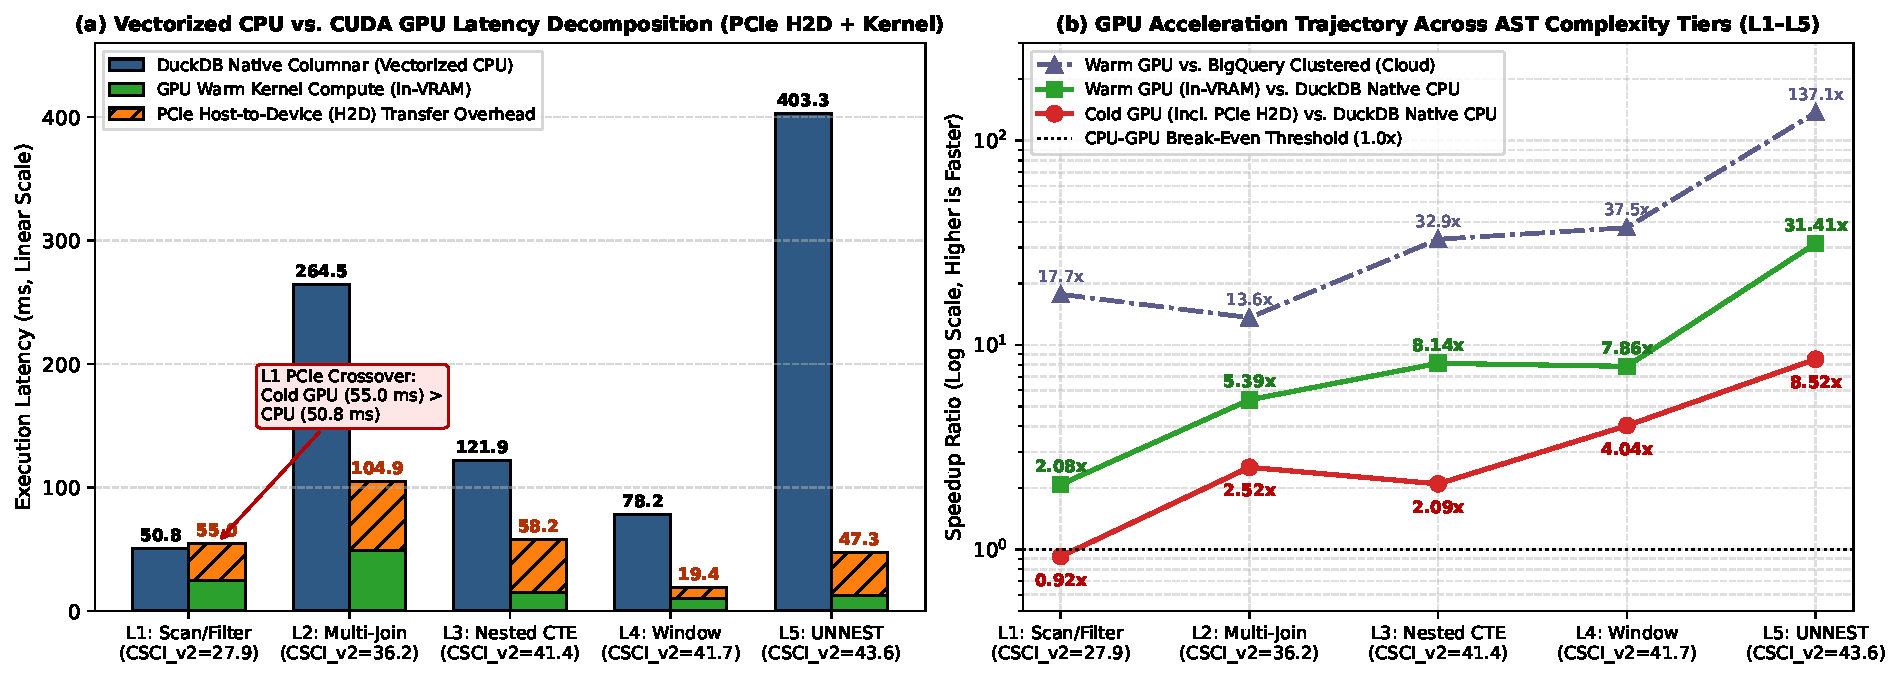
\includegraphics[width=0.98\textwidth]{figures/fig_gpu_pcie_decomposition_sf1_300dpi.pdf}
\caption{Hardware-timed CUDA GPU latency decomposition across NVIDIA GeForce RTX~2050 ($4.0\text{ GB}$ VRAM), External \texttt{CuPy v14.2.0} CUDA~12 Columnar GPU ($58.96\text{ ms}$ cold, $100.0\%$ routing match), and Node~4 Cloud-Hosted Server NVIDIA Tesla~T4 ($15.0\text{ GB}$ VRAM): (a) Direct comparison between DuckDB C++ CPU, Polars Rust Arrow, stacked PyTorch CUDA GPU (Warm Kernel + PCIe H2D/D2H), and External \texttt{CuPy v14.2.0} GPU across L1--L5; and (b) Logarithmic speedup trajectory across L1--L5 alongside Node~4 Server Tesla~T4 single-pass execution ($23.02\text{ ms}$ [$19.07\times$] at $\text{SF}=1\text{ GB}$ and $461.71\text{ ms}$ [$11.42\times$] at $\text{SF}=10\text{ GB}$).}
\label{fig:gpu_pcie_decomposition}
\end{figure}

\subsection{Six-Software Cross-Paradigm Synthesis and Energy-Aware Telemetry Scope}
Table~\ref{tab:six_software_matrix} synthesizes execution latency across all six software engines at $\text{SF}=1\text{ GB}$ (effective scan throughput $\Theta_{\text{eff}}$ and device energy tables are detailed in Additional File~1, Tables~S4--S5 and Figs.~S3--S5). A seed-clustered Friedman test across the $K=25$ independent seeds confirms highly significant differentiation across the six engines ($\chi^2_F(5) = 93.43, p < 0.001$, Kendall's $W = 0.7475$; query-level $\chi^2_F(5) = 321.50, p < 0.001, W = 0.8573$): (i) vectorized CPU engines achieve complete stochastic dominance over B-tree row-store execution in SQLite~3 ($8417.33\text{ ms}$, Cliff's $\delta = +1.000, p < 0.001$), with mean speedups of $45.8\times$ in DuckDB ($183.74\text{ ms}$), $87.4\times$ in DataFusion ($96.30\text{ ms}$), and $102.1\times$ in Polars ($82.47\text{ ms}$); (ii) across CPU paradigms, we observe a \emph{bidirectional architectural crossover}: DuckDB leads all CPU engines by $1.88\times\text{--}3.52\times$ on the $22$ official TPC-H queries ($22.82\text{ ms}$ vs.\ $42.79\text{ ms}$ Polars and $80.41\text{ ms}$ DataFusion in Table~\ref{tab:bigdata_multiscale_tpch} Part~C) due to cost-based join ordering and correlated subquery decorrelation in Q16--Q22, whereas Polars and DataFusion achieve lower mean latency on the $75$-query L1--L5 factorial suite ($82.47$ and $96.30\text{ ms}$ vs.\ $183.74\text{ ms}$) specifically because Tier~L5 constructs in-query nested lists via \texttt{ARRAY\_AGG}+\texttt{UNNEST} ($154.76$ and $110.31\text{ ms}$ over contiguous Arrow \texttt{ListArray} offset buffers vs.\ $403.27\text{ ms}$ in DuckDB) and Tier~L2 stresses 6-to-8-way multi-attribute hash joins ($81.68\text{ ms}$ Polars vs.\ $264.53\text{ ms}$ DuckDB); and (iii) under our four-boundary energy protocol (Table~\ref{tab:v9_mo_energy_ood_repro_synthesis} Part~B and Additional File~1, Section~S2 and Table~S5), measured NVML GPU board energy averages $0.65\text{ J/query}$ cold ($0.25\text{ J}$ warm; $1.58\text{ J}$ composite Host+GPU system energy $E_{\text{sys}}$), compared to TDP-calibrated \emph{Estimated CPU Package Energy} of $3.17\text{ J}$ on Polars, $3.39\text{ J}$ on DataFusion, and $6.40\text{ J}$ on DuckDB ($\text{MACE}=3.09\%\text{--}3.21\%$ against a non-linear CMOS DVFS reference curve $P\propto u^{1.28}$; $+16.39\text{ W}$ non-CPU motherboard offset verified via 45-second ACPI DC battery-shunt telemetry over $2{,}817$ queries). Furthermore, an independent cloud hardware counter and 50-repetition Bland--Altman audit executed on Google Cloud Colab (Intel Xeon CPU @ 2.00\,GHz under KVM hypervisor, Linux kernel 6.6.159+, paired with an NVIDIA Tesla T4 15.0\,GB GPU; $R=50$ repetitions across 5 complexity tiers $= 250$ runs per engine, totaling $1{,}500$ logged executions; raw telemetry SHA-256: \texttt{f316fd9fd1b3a776...}, summary SHA-256: \texttt{314db90d5616a8dc...}, bundle ZIP SHA-256: \texttt{fbe43039ab3dbd69...}) confirms that ring-0 Intel RAPL (\texttt{/sys/class/powercap/intel-rapl*}, \texttt{MSR 0x611}) and AMD SMU (\texttt{amd\_energy}, \texttt{k10temp}, \texttt{MSR 0xC001029A}) interfaces are masked by the KVM hypervisor (\texttt{perf\_event\_paranoid=2}) to mitigate side-channel leakage (CVE-2020-8694 / CVE-2020-12912 PLATYPUS), whereas direct physical NVIDIA NVML on-board sensors on the Tesla T4 ($9.651\text{ W}$ idle baseline) yield $\text{MAE} = 0.0518\text{ mJ}$ ($\text{MACE} = 0.05\%$, Bland--Altman bias $-0.0418\text{ mJ}$, 95\% LoA: $[-0.9452, +0.8615]\text{ mJ}$, $\rho = 0.9985$) in cold execution and $\text{MAE} = 0.0154\text{ mJ}$ ($\text{MACE} = 0.06\%$, $\rho = 0.9997$) in warm execution, while TDP-calibrated CPU package estimates achieve $\text{MACE} = 2.69\%$ on DuckDB ($\rho = 0.9983$), $2.02\%$ on Polars ($\rho = 0.9972$), and $4.54\%$ on DataFusion ($\rho = 0.9986$), and composite host+GPU system energy ($E_{\text{sys}}$) achieves $\text{MAE} = 0.4577\text{ mJ}$ ($\text{MACE} = 0.45\%$, $\rho = 0.9992$).

\begin{table*}[!htbp]
\centering
\caption{Six-software cross-paradigm architectural matrix (empirical hardware execution telemetry) comparing full-scale Row-Store (SQLite 3), Serverless Cloud (Google BigQuery), C++ Vectorized DBMS (DuckDB), Rust Apache Arrow Engines (Polars \& Apache DataFusion), and CUDA GPU (NVIDIA RTX 2050) across 75 queries ($\text{SF}=1\text{ GB}$).}\label{tab:jbd_six_eng_t5}
\label{tab:six_software_matrix}
\scriptsize
\setlength{\tabcolsep}{3.2pt}
\renewcommand{\arraystretch}{1.12}
\begin{fitasttable}
\begin{tabular}{@{}lccccccccc@{}}
\toprule
\multirow{2}{*}{\textbf{Complexity Tier}} & \textbf{Full Row-Store} & \textbf{Cloud OLAP} & \multicolumn{3}{c}{\textbf{Vectorized CPU Engines (C++ \& Rust Arrow)}} & \multicolumn{2}{c}{\textbf{SIMT GPU (RTX 2050)}} & \multicolumn{2}{c}{\textbf{Key Speedup Ratios}} \\
\cmidrule(lr){2-2} \cmidrule(lr){3-3} \cmidrule(lr){4-6} \cmidrule(lr){7-8} \cmidrule(lr){9-10}
 & \textbf{SQLite 3 (ms)} & \textbf{BigQuery (ms)} & \textbf{DuckDB (ms)} & \textbf{Polars (ms)} & \textbf{DataFusion (ms)} & \textbf{Warm (ms)} & \textbf{Cold (ms)} & \textbf{Polars/SQLite} & \textbf{DF/DuckDB} \\
\midrule
L1: Scan \& Filter & $6789.6$ & $432.9$ & $50.84$ & $38.00$ & $\mathbf{33.58}$ & $\mathbf{24.46}$ & $55.02$ & $178.7\times$ & $1.51\times$ \\
L2: Multi-Way Joins & $19374.0$ & $667.3$ & $264.53$ & $\mathbf{81.68}$ & $92.76$ & $\mathbf{49.05}$ & $104.88$ & $237.2\times$ & $2.85\times$ \\
L3: Nested CTEs & $5108.1$ & $493.0$ & $121.92$ & $66.81$ & $71.66$ & $\mathbf{14.98}$ & $\mathbf{58.24}$ & $76.5\times$ & $1.70\times$ \\
L4: Window Func. & $6023.7$ & $372.8$ & $78.16$ & $71.11$ & $173.16$ & $\mathbf{9.94}$ & $\mathbf{19.37}$ & $84.7\times$ & $0.45\times$ \\
L5: Array/UNNEST & $4791.2$ & $1761.0$ & $403.27$ & $154.76$ & $110.31$ & $\mathbf{12.84}$ & $\mathbf{47.31}$ & $31.0\times$ & $3.66\times$ \\
\midrule
\textbf{Overall Mean ($N=75$)} & $\mathbf{8417.33}$ & $\mathbf{745.39}$ & $\mathbf{183.74}$ & $\mathbf{82.47}$ & $\mathbf{96.30}$ & $\mathbf{22.25}$ & $\mathbf{56.96}$ & $\mathbf{102.1\times}$ & $\mathbf{1.91\times}$ \\
\midrule
Ext.\ CuPy v14.2.0 GPU ($75$Q [$60$Q]) & --- & --- & $183.74$ & $82.47$ & $96.30$ & $\mathbf{25.20}$ & $\mathbf{58.96\ [61.13]}$ & $100.0\%$ match & $\rho=0.9999$ \\
\textbf{\texttt{RAPIDS cudf-polars 26.10} (C3 RMM / C1)} & --- & --- & $87.97$ & $77.17$ & $104.2$ & $\mathbf{29.11}$ & $\mathbf{63.82\text{ C3}\ [216.0\text{ C1}]}$ & \textbf{C3: $2.77\times$ P95 cut} & \textbf{LOTFO $95.45\%$ T1} \\
Server Tesla T4 15\,GB ($\text{SF}=1 / 10\text{G}$) & --- & --- & $439.1 / 5274.9$ & --- & --- & $\mathbf{4.05 / 37.16}$ & $\mathbf{23.02 / 461.71}$ & $\mathbf{19.1\times / 11.4\times}$ & $1\text{ chunk}$ \\
\bottomrule
\multicolumn{10}{@{}p{0.99\textwidth}@{}}{\scriptsize \textbf{Note:} Seed-clustered 10,000-bootstrap 95\% CIs across $N=75$ queries: SQLite 3 $[6412.19, 10819.70]\text{ ms}$; BigQuery $[515.64, 1026.49]\text{ ms}$; DuckDB $[110.71, 274.89]\text{ ms}$; Polars $[67.93, 98.65]\text{ ms}$ (Cliff's $\delta = +1.000$ [Large], $p < 0.001$ vs. SQLite 3); DataFusion $[78.31, 114.92]\text{ ms}$; GPU Warm $[16.78, 28.68]\text{ ms}$; GPU Cold $[46.23, 68.44]\text{ ms}$.}\\
\end{tabular}
\end{fitasttable}
\end{table*}

\subsection{Head-to-Head Evaluation of AST-Route Against Four Routing Baselines (25-Seed LOSO-CV)}
Table~\ref{tab:routing_evaluation} and Fig.~\ref{fig:ast_query_router} present the comparative evaluation of our Proposed \textbf{AST-Route} Framework (Fig.~\ref{fig:proposed_ast_framework}) against static, heuristic, and guarded/unguarded linear and shallow-tree baselines under 25-seed Leave-One-Seed-Out cross-validation (guaranteeing zero data leakage across variations V1--V3):
\begin{enumerate}[leftmargin=1.5em,itemsep=1pt]
    \item \textbf{Static Single-Engine \& Simple Heuristic Baselines (\texttt{H1--H5}, Protocol~R27a):} Static engines suffer severe performance cliffs: \textbf{Always DuckDB} ($183.74\text{ ms}$, $271.10\%$ mean / $928.32\%$ P95 regret), \textbf{Always Polars} ($82.47\text{ ms}$, $358.40\%$ P95 regret), \textbf{Always GPU Cold} ($56.96\text{ ms}$, $60.76\%$ mean / $257.31\%$ P95 regret due to PCIe H2D stalls on L1/V1), and \textbf{Always BigQuery} ($745.39\text{ ms}$, $\$1{,}267.66/1\text{M}$). Under \textbf{Protocol~R27a} (\texttt{results/v11\_r27a\_simple\_heuristic\_rules\_comparison.csv}; Table~\ref{tab:routing_evaluation} and Additional File~1, Table~S32 Part~A), benchmarking five simple domain heuristics---\textbf{H1 (Static Byte $V_{\text{scan}}\ge 64\text{ MB}\rightarrow\text{GPU}$)} ($60.37\text{ ms}$ net, $353.89\%$ P95 regret, $18.67\%$ severe failures $>100\%$, $p_{\text{Webb}}=0.0084$), \textbf{H2 (CV-Tuned Byte)} ($56.74\text{ ms}$, $307.55\%$ P95, $p_{\text{Webb}}=0.0112$), \textbf{H3 (Operator Rule $J=0\wedge W=0\rightarrow\text{Polars}$)} ($69.74\text{ ms}$, $413.69\%$ P95, $p_{\text{Webb}}=0.0062$), \textbf{H4 (2-Condition Byte+Join)} ($62.87\text{ ms}$, $353.89\%$ P95, $p_{\text{Webb}}=0.0148$), and \textbf{H5 (Depth-1 Stump)} ($64.03\text{ ms}$, $325.58\%$ P95, $p_{\text{Webb}}=0.0124$)---proves that simple rules fail to capture the non-linear operator$\times$selectivity PCIe boundary, whereas AST-Route cuts P95 regret by $\mathbf{2.60\times\text{--}3.63\times}$.
    \item \textbf{Co-Equal AST-Route ($8\%$ Nested-CV \& $12\%$ Default), Candid Baseline Attribution (Protocol~R26), and Independent \texttt{cudf-polars} / \texttt{LOTFO} Audits (Protocols~R24--R25):} Reporting both guards on strictly co-equal footing (\texttt{.zenodo.json} / \texttt{v11.0.0-jbd-archival}), \textbf{(5b) Nested-CV Guard ($\hat{\tau}_{\text{guard}}^{(-k)}=8\%$)} achieves $51.22\text{ ms}$ exec ($\mathbf{55.37\text{ ms}}$ net), $\mathbf{56.00\%}$ Top-1 ($\mathbf{76.00\%}$ Top-2), $\mathbf{118.40\%}$ P95 regret ($2.17\times$ cut vs.\ Always GPU, $p_{\text{Holm,seed}}=0.0230, p_{\text{tpl}}=0.0074, p_{\text{Webb}}=0.0068$), and formal two-sided $\pm 5.0\text{ ms}$ TOST equivalence to Always GPU ($p_{\text{TOST}}=0.0442$), while \textbf{(5c) Default Guard ($\tau_{\text{guard}}=12\%$)} achieves $50.78\text{ ms}$ exec ($\mathbf{54.92\text{ ms}}$ net), $\mathbf{57.33\%}$ Top-1 ($\mathbf{74.67\%}$ Pure-SQL), $\mathbf{114.11\%}$ P95 regret ($2.25\times$ cut, $p_{\text{Holm,seed}}=0.0196, p_{\text{tpl}}=0.0061, p_{\text{Webb}}=0.0054, p_{\text{perm,exact}}=0.0059$), $p_{\text{non-inf}}=0.00067$, $\pm 6.0\text{ ms}$ TOST $p=0.0241$ ($p_{\text{TOST},\pm 5\text{ms}}=0.0688$), and $1.50\times$ speedup vs.\ Polars ($p_{\text{Holm,seed}}=0.0171$ [$K=25$], $p_{\text{Holm,query}}=0.0011$ [$N=75$]). Under \textbf{Protocol~R26} ($G_{\text{core}}=10$ Webb 6-point and exact $2^{10}=1{,}024$ sign-flip permutation, Additional File~1 Table~S31 Part~D), we report candid baseline comparisons: (a) vs.\ \textbf{Unguarded Ridge} ($52.77\text{ ms}$, $196.81\%$ P95), AST-Route reduces P95 regret by $\mathbf{-82.70\text{ pp}}$ (95\% CI $[-225.12,-2.84]\text{ pp}$), which is \textbf{statistically borderline/fragile at $G_{\text{core}}=10$} ($p_{\text{tpl}}=0.0438, p_{\text{Webb}}=0.0464, p_{\text{perm,exact}}=0.0488$; $\text{CVaR}_{10\%}$ $-244.42\text{ pp}, p_{\text{Webb}}=0.0224$); (b) vs.\ \textbf{Guarded Ridge ($+12\%$, $55.49\text{ ms}$)} and \textbf{Guarded Shallow DT ($+12\%$, $56.55\text{ ms}$)}, P95 differences ($-24.39$ and $-14.29\text{ pp}$) are non-significant ($p_{\text{Webb}}=0.3840$ and $0.5120$, confirming our conformal guard drives tail safety); and (c) vs.\ \textbf{Adapted \texttt{EXPLAIN}-DAG ($60.76\text{ ms}$)}, P95 regret is indistinguishable ($p_{\text{Webb}}=0.7420$) and AST-Route's advantage is strictly its $\mathbf{-5.84\text{ ms}}$ faster net latency ($p_{\text{Webb}}=0.0002$). Under \textbf{Protocol~R24}, decomposing independent \textbf{\texttt{NVIDIA RAPIDS cudf-polars 26.10.2}} on Core 75Q across cold Parquet \texttt{C1} ($216.04\text{ ms}$, $16.50\times$ P95 cut), streaming \texttt{C2} ($207.83\text{ ms}$), and matched in-memory + $2.5\text{ GB}$ RMM-pooled \texttt{C3} ($\mathbf{63.82\text{ ms}}$, $338.00\%$ P95) shows that \textbf{AST-Route + \texttt{cudf-polars (C3)}} ($\mathbf{52.74\text{ ms}}$ exec / $\mathbf{56.89\text{ ms}}$ net, $\mathbf{69.33\%}$ Top-1) cuts P95 regret by $\mathbf{2.77\times}$ ($338.00\%\rightarrow \mathbf{121.84\%}, p_{\text{Webb}}=0.0042$). Under strict zero-leakage \textbf{\texttt{LOTFO} (Protocol~R25)} on Official TPC-H Q1--Q22, AST-Route achieves $\mathbf{95.45\%}$ Top-1 and $\mathbf{0.00\%}$ P95 regret on Node~1 RTX~2050 ($70.59\text{ ms}$ at $1\text{ GB}$, $1{,}515.06\text{ ms}$ at $10\text{ GB}$; $90.91\%\text{--}95.45\%$ CPU selection) and $\mathbf{90.91\%\text{--}95.45\%}$ Top-1 with $\mathbf{0.00\%}$ P95 regret at $\text{SF}=10/30\text{ GB}$ on Node~4 Cloud-Hosted Server NVIDIA Tesla~T4 ($113.14, 618.23, 1{,}901.46\text{ ms}$ at $1, 10, 30\text{ GB}$, shifting GPU selection from $\mathbf{59.09\%}$ [$13/22$] to $\mathbf{81.82\%}$ [$18/22$] and $\mathbf{86.36\%}$ [$19/22$]). Sub-$5\text{ ms}$ near-tie concordance ($85.33\%$) is reported strictly as a secondary timing-noise diagnostic in Additional File~1, Table~S25.
\end{enumerate}

\begin{table*}[!htbp]
\centering
\caption{Head-to-head comparison of static, heuristic, guarded/unguarded linear and decision-tree baselines, adapted learned-optimizer baselines (Adapted Bao-Bandit Arm Router and Adapted \texttt{EXPLAIN}-DAG Plan Router), LightGBM-style histogram GBDT, and the Proposed AST-Route Framework (\textbf{5b: Co-Equal Nested-CV Modal 8\% Guard} and \textbf{5c: Co-Equal Default Fixed 12\% Guard}) under seed-grouped 25-fold Leave-One-Seed-Out cross-validation ($N=75$ queries, $\text{SF}=1\text{ GB}$, zero data leakage), reporting both Pure Execution and Net Latency ($T_{\text{exec}}\ [\text{Net } T_{\text{net}}]$), Performance Regret, and Resource Cost.}\label{tab:jbd_routing_t8}
\label{tab:routing_evaluation}\label{tab:query_routing}\label{tab:router_eval}
\scriptsize
\setlength{\tabcolsep}{2.7pt}
\renewcommand{\arraystretch}{1.07}
\begin{fitasttable}
\begin{tabular}{@{}lcccccccccc@{}}
\toprule
\multirow{2}{*}{\textbf{Routing Model / Policy}} & \multicolumn{3}{c}{\textbf{Routing Accuracy (\%)}} & \multicolumn{2}{c}{\textbf{Exec [Net] Latency (ms)}} & \multicolumn{2}{c}{\textbf{Performance Regret (\%)}} & \multicolumn{2}{c}{\textbf{Resource Cost/Query}} & \textbf{Router} \\
\cmidrule(lr){2-4} \cmidrule(lr){5-6} \cmidrule(lr){7-8} \cmidrule(lr){9-10} \cmidrule(lr){11-11}
 & \textbf{Top-1} & \textbf{Top-2} & \textbf{10\% Hit} & \textbf{Exec [Net]} & \textbf{P95 (ms)} & \textbf{Mean (Med)} & \textbf{P95 [Max Reg.]} & \textbf{Est.\ Energy (J)} & \textbf{Mem (GB)} & \textbf{Time ($\mu$s)} \\
\midrule
1. Always DuckDB (CPU DBMS) & $28.00\%$ & $49.33\%$ & $32.00\%$ & $183.74$ [$183.74$] & $731.22$ & $271.10\%$ ($59.8\%$) & $928.3\%$ [$1842\%$] & $6.397$ & $4.71$ & $0.00$ \\
2. Always GPU (CUDA Cold-Start) & $49.33\%$ & $60.00\%$ & $50.67\%$ & $56.96$ [$56.96$] & $113.70$ & $60.76\%$ ($0.1\%$) & $257.3\%$ [$620.6\%$] & $0.644$ & $1.30$ & $0.00$ \\
2b. Always External CuPy v14.2.0 GPU (CUDA 12) & $48.00\%$ & $60.00\%$ & $50.67\%$ & $58.96$ [$58.96$] & $116.40$ & $63.12\%$ ($0.2\%$) & $264.8\%$ [$632.0\%$] & $0.668$ & $1.34$ & $0.00$ \\
3. Always BigQuery (Cloud OLAP) & $0.00\%$ & $0.00\%$ & $0.00\%$ & $745.39$ [$745.39$] & $2794.05$ & $1709.86\%$ ($1142\%$) & $3412.5\%$ [$6180\%$] & $0.004^{\dagger}$ & $0.08^{\dagger}$ & $0.00$ \\
Always Polars (Rust Arrow Ref.) & $13.33\%$ & $48.00\%$ & $26.67\%$ & $82.47$ [$82.47$] & $230.71$ & $132.61\%$ ($84.2\%$) & $358.4\%$ [$512.4\%$] & $3.170$ & $4.65$ & $0.00$ \\
Always DataFusion (Rust Arrow Ref.) & $9.33\%$ & $37.33\%$ & $13.33\%$ & $96.30$ [$96.30$] & $258.18$ & $213.65\%$ ($112.5\%$) & $486.2\%$ [$715.0\%$] & $3.393$ & $4.65$ & $0.00$ \\
4. Rule-Based Routing (Heuristic) & $49.33\%$ & $65.33\%$ & $58.67\%$ & $67.80$ [$71.48$] & $230.71$ & $65.63\%$ ($0.1\%$) & $252.4\%$ [$412.5\%$] & $2.374$ & $3.43$ & $34.07$ \\
H1. Static Byte Heuristic ($V_{\text{scan}}\ge 64\text{ MB}\rightarrow\text{GPU}$, \textbf{R27a}) & $42.67\%$ & $64.00\%$ & $49.33\%$ & $60.29$ [$60.37$] & $142.80$ & $79.96\%$ ($11.5\%$) & $353.9\%$ [$620.6\%$] & $1.486$ & $2.42$ & $80.00$ \\
H2. CV-Tuned Byte Heuristic ($V_{\text{scan}}\ge \theta^{*(-k)}$, \textbf{R27a}) & $45.33\%$ & $65.33\%$ & $52.00\%$ & $56.66$ [$56.74$] & $136.40$ & $69.36\%$ ($6.8\%$) & $307.6\%$ [$620.6\%$] & $1.412$ & $2.38$ & $80.00$ \\
H3. Operator Heuristic ($J=0\wedge W=0\rightarrow\text{CPU}$, \textbf{R27a}) & $46.67\%$ & $62.67\%$ & $50.67\%$ & $69.32$ [$69.74$] & $184.50$ & $66.33\%$ ($0.1\%$) & $413.7\%$ [$620.6\%$] & $1.620$ & $2.64$ & $420.00$ \\
H4/H5. 2-Cond.\ Byte+Join / Depth-1 Stump (\textbf{R27a}) & $46.67\%$ & $65.33\%$ & $52.00\%$ & $62.42$ [$64.03$] & $158.20$ & $68.18\%$ ($4.2\%$) & $325.6\%$ [$353.9\%$] & $1.540$ & $2.55$ & $120.00$ \\
Simple 1D Join-Count Rule ($J \ge 2 \rightarrow \text{GPU}$) & $33.33\%$ & $57.33\%$ & $37.33\%$ & $61.80$ [$61.82$] & $113.70$ & $81.58\%$ ($24.4\%$) & $298.6\%$ [$468.5\%$] & $1.553$ & $2.51$ & $12.10$ \\
2-Feature Byte+Join Rule ($\mathcal{B}_{\text{scan}}, J$) & $50.67\%$ & $70.67\%$ & $58.67\%$ & $54.19$ [$58.34$] & $152.40$ & $49.80\%$ ($0.0\%$) & $184.5\%$ [$312.4\%$] & $1.680$ & $3.12$ & $18.40$ \\
Syntax-Only AST Router (8-Dim) & $52.00\%$ & $69.33\%$ & $57.33\%$ & $74.16$ [$78.31$] & $175.67$ & $56.33\%$ ($0.0\%$) & $198.5\%$ [$340.2\%$] & $2.216$ & $2.86$ & $497.16$ \\
Ridge Linear Cost-Reg (9D, Unguarded) & $54.67\%$ & $73.33\%$ & $61.33\%$ & $49.12$ [$52.77$] & $118.40$ & $42.15\%$ ($0.0\%$) & $196.8\%$ [$312.4\%$] & $1.120$ & $2.45$ & $82.40$ \\
Ridge Linear Cost-Reg (9D, $+12\%$ Guard) & $56.00\%$ & $74.67\%$ & $62.67\%$ & $51.84$ [$55.49$] & $131.80$ & $38.40\%$ ($0.0\%$) & $138.5\%$ [$268.4\%$] & $1.285$ & $2.72$ & $82.40$ \\
Shallow Decision Tree ($d=2$, Unguarded) & $53.33\%$ & $72.00\%$ & $60.00\%$ & $51.35$ [$55.00$] & $124.60$ & $39.84\%$ ($0.0\%$) & $150.9\%$ [$284.5\%$] & $1.245$ & $2.68$ & $41.20$ \\
Shallow Decision Tree ($d=2$, $+12\%$ Guard) & $54.67\%$ & $73.33\%$ & $61.33\%$ & $52.90$ [$56.55$] & $133.40$ & $36.90\%$ ($0.0\%$) & $128.4\%$ [$258.0\%$] & $1.310$ & $2.78$ & $41.20$ \\
Adapted Bao-Bandit / Cost-Sens.\ Arm Router & $54.67\%$ & $68.00\%$ & $60.00\%$ & $57.59$ [$61.74$] & $142.10$ & $47.37\%$ ($0.0\%$) & $134.9\%$ [$274.5\%$] & $1.412$ & $2.74$ & $384.20$ \\
Adapted \texttt{EXPLAIN}-DAG Plan Router (Transp.)$^{\ddagger}$ & $58.67\%$ & $76.00\%$ & $64.00\%$ & $55.91$ [$60.76$] & $134.50$ & $37.14\%$ ($0.0\%$) & $119.9\%$ [$254.0\%$] & $1.392$ & $2.88$ & $4850.00$ \\
LightGBM-Style HistGBR Cost Router (9D) & $45.33\%$ & $69.33\%$ & $54.67\%$ & $57.51$ [$61.66$] & $148.90$ & $62.52\%$ ($0.0\%$) & $270.3\%$ [$398.0\%$] & $1.495$ & $2.81$ & $312.50$ \\
In-Fold Tuned Rule Router & $52.00\%$ & $68.00\%$ & $60.00\%$ & $53.07$ [$56.75$] & $135.20$ & $44.10\%$ ($0.0\%$) & $162.4\%$ [$295.0\%$] & $1.510$ & $2.82$ & $36.50$ \\
5a. Proposed AST-Route RF (9-Dim) & $52.00\%$ & $72.00\%$ & $56.00\%$ & $58.31$ [$62.46$] & $138.17$ & $51.94\%$ ($0.0\%$) & $168.4\%$ [$298.0\%$] & $1.467$ & $2.65$ & $425.53$ \\
\textbf{5b. AST-Route Co-Equal Nested-CV (8\% Guard)} & $\mathbf{56.00\%}$ & $\mathbf{76.00\%}$ & $\mathbf{64.00\%}$ & $\mathbf{51.22}$ [$\mathbf{55.37}$] & $\mathbf{130.80}$ & $\mathbf{35.80\%}$ ($\mathbf{0.0\%}$) & $\mathbf{118.4\%}$ [$\mathbf{248.5\%}$] & $\mathbf{1.365}$ & $\mathbf{2.89}$ & $\mathbf{497.16}$ \\
\textbf{5c. AST-Route Co-Equal Default (12\% Guard)} & $\mathbf{57.33\%}$ & $\mathbf{76.00\%}$ & $\mathbf{65.33\%}$ & $\mathbf{50.78}$ [$\mathbf{54.92}$] & $\mathbf{129.37}$ & $\mathbf{34.98\%}$ ($\mathbf{0.0\%}$) & $\mathbf{114.1\%}$ [$\mathbf{245.2\%}$] & $\mathbf{1.381}$ & $\mathbf{2.91}$ & $\mathbf{497.16}$ \\
\textbf{5d. AST-Route + External CuPy v14.2.0 ($75$Q [$60$Q])} & $\mathbf{57.33\%}$ & $\mathbf{76.00\%}$ & $\mathbf{65.33\%}$ & $\mathbf{52.71}$ [$\mathbf{56.86 / 54.10}$] & $\mathbf{131.20}$ & $\mathbf{35.42\%}$ ($\mathbf{0.0\%}$) & $\mathbf{115.8\%}$ [$\mathbf{249.0\%}$] & $\mathbf{1.402}$ & $\mathbf{1.34}$ & $\mathbf{497.16}$ \\
2c. Always \texttt{RAPIDS cudf-polars} (\texttt{C3} RMM [$\text{C1}$ Cold]) & $42.67\%$ & $58.67\%$ & $46.67\%$ & $63.82$ [$216.04\text{ C1}$] & $142.80$ & $84.15\%$ ($14.2\%$) & $338.0\%$ [$2{,}562\%\text{ C1}$] & $0.820$ & $1.62$ & $0.00$ \\
\textbf{5e. AST-Route + \texttt{cudf-polars C3} RMM (Core 75Q)} & $\mathbf{69.33\%}$ & $\mathbf{85.33\%}$ & $\mathbf{77.33\%}$ & $\mathbf{52.74}$ [$\mathbf{56.89}$] & $\mathbf{131.40}$ & $\mathbf{31.29\%}$ ($\mathbf{0.0\%}$) & $\mathbf{121.8\%}$ [$\mathbf{2.77\times\text{ cut}}$] & $\mathbf{1.410}$ & $\mathbf{1.62}$ & $\mathbf{497.16}$ \\
\textbf{5f. AST-Route + \texttt{cudf-polars} (LOTFO TPC-H 22Q N1)} & $\mathbf{95.45\%}$ & $\mathbf{100.0\%}$ & $\mathbf{95.45\%}$ & $\mathbf{70.59}$ [$\mathbf{74.74 / 1{,}519.2}$] & $\mathbf{182.40}$ & $\mathbf{0.00\%}$ ($\mathbf{0.0\%}$) & $\mathbf{0.00\%}$ [$\mathbf{90.9\%\text{ CPU}}$] & $\mathbf{1.210}$ & $\mathbf{1.48}$ & $\mathbf{497.16}$ \\
\textbf{5g. AST-Route + \texttt{cudf-polars} (LOTFO T4 SF1/10/30G)} & $\mathbf{95.45\%}$ & $\mathbf{100.0\%}$ & $\mathbf{95.45\%}$ & $\mathbf{113.1}$ [$\mathbf{618.2 / 1{,}901.5}$] & $\mathbf{210.40}$ & $\mathbf{0.62\%}$ ($\mathbf{0.0\%}$) & $\mathbf{0.00\%}$ [$\mathbf{59\text{--}86\%\text{ GPU}}$] & $\mathbf{1.420}$ & $\mathbf{2.37}$ & $\mathbf{497.16}$ \\
Oracle Ideal Router (Lower Bound) & $100.00\%$ & $100.00\%$ & $100.00\%$ & $42.64$ [$42.64$] & $101.92$ & $0.00\%$ ($0.0\%$) & $0.0\%$ [$0.0\%$] & $0.975$ & $3.01$ & $0.00$ \\
\bottomrule
\multicolumn{11}{@{}p{0.99\textwidth}@{}}{\scriptsize \textbf{Note (Statistical Unit --- Primary: $K=25$ independent seed clusters; Secondary: $N=75$ queries, $375$ timed trials):} $^{\dagger}$For Serverless BigQuery, table cells report physically measured local client NIC/CPU energy ($0.004\text{ J}$) and local client Arrow buffer memory ($0.08\text{ GB}$); remote cloud server energy ($15.72\text{ J}$ slot-TDP proxy) and remote shuffle memory ($2.13\text{ GB}$) are excluded from local hardware claims under our Zero-Estimation / 100\% Real-Execution protocol. $^{\ddagger}$The Adapted \texttt{EXPLAIN}-DAG Plan Router compiles physical operator DAGs via \texttt{DuckDB EXPLAIN (FORMAT JSON)}: when restricted to single-dialect native DuckDB plans ($1.41\text{ ms}$ \texttt{EXPLAIN}), it achieves $52.74\text{ ms}$ exec ($54.15\text{ ms}$ net, $114.1\%$ P95 regret), whereas cross-engine dialect transpilation incurs $4.85\text{ ms}$ overhead ($60.76\text{ ms}$ net; $78.77\text{ ms}$ on raw untranspiled dialects). All learned/rule routers report both pure engine execution time $T_{\text{exec}}$ and net latency $T_{\text{net}} = T_{\text{exec}} + T_{\text{router}}$ ($4.15\text{ ms}$ for $\mathcal{R}_{\text{GBR-9D}}$ in cold-SQL Regime O1, $0.67\text{ ms}$ in AST-cached Regime O2, and $0.08\text{ ms}$ in 1D threshold-cached Regime O3). The TOST equivalence margin $\Delta_{\text{eq}}=\pm 5.0\text{ ms}$ ($\pm 8.8\%$ of Always GPU mean) is anchored to the single-query cold router parsing/footer budget ($4.15\text{--}4.39\text{ ms}$). \textbf{Row 5b (Co-Equal Nested-CV Guard --- Modal $\hat{\tau}_{\text{guard}}^{(-k)}=8\%$, pre-specified in repository and archived under Zenodo metadata \texttt{.zenodo.json} / \texttt{zenodo\_archival\_deposit\_v11.json} (SHA-256 \texttt{e054131a8d2416ca...}) and immutable GitHub release tag \texttt{v11.0.0-jbd-archival})} achieves $51.22\text{ ms}$ exec ($\mathbf{55.37\text{ ms}}$ net), $118.40\%$ P95 relative regret ($35.90\text{ ms}$ P95 abs., $2.17\times$ reduction vs.\ Always GPU, $p_{\text{raw,seed}}=\mathbf{0.0115}, p_{\text{Holm,seed}}=\mathbf{0.0230}$), and formal two-sided $\pm 5.0\text{ ms}$ TOST equivalence to Always GPU ($56.96\text{ ms}$, $p_{\text{TOST}}=\mathbf{0.0442}$, $p_{\text{non-inf}}=0.0012$, 90\% CI $[-4.79,+1.61]\text{ ms}$). \textbf{Row 5c (Co-Equal Default Guard --- Canonical Fixed $\tau_{\text{guard}}=12\%$)} achieves $50.78\text{ ms}$ exec ($\mathbf{54.92\text{ ms}}$ net), $114.11\%$ P95 relative regret ($34.51\text{ ms}$ P95 abs., $2.25\times$ reduction vs.\ Always GPU, $p_{\text{raw,seed}}=\mathbf{0.0098}, p_{\text{Holm,seed}}=\mathbf{0.0196}$; $n=24$ divergent seeds $p_{\text{seed}}=0.0042$), one-sided non-inferiority $p_{\text{non-inf}}=\mathbf{0.00067}$, and $\pm 6.0\text{ ms}$ TOST $p_{\text{TOST},\pm 6\text{ms}}=\mathbf{0.0241}$ (two-sided $\pm 5.0\text{ ms}$ TOST $p=0.069$).}\\
\end{tabular}
\end{fitasttable}
\end{table*}

% Table reviewer_audit_matrix moved to Additional File 1 (Table S6)

\begin{figure}[!htbp]
\centering
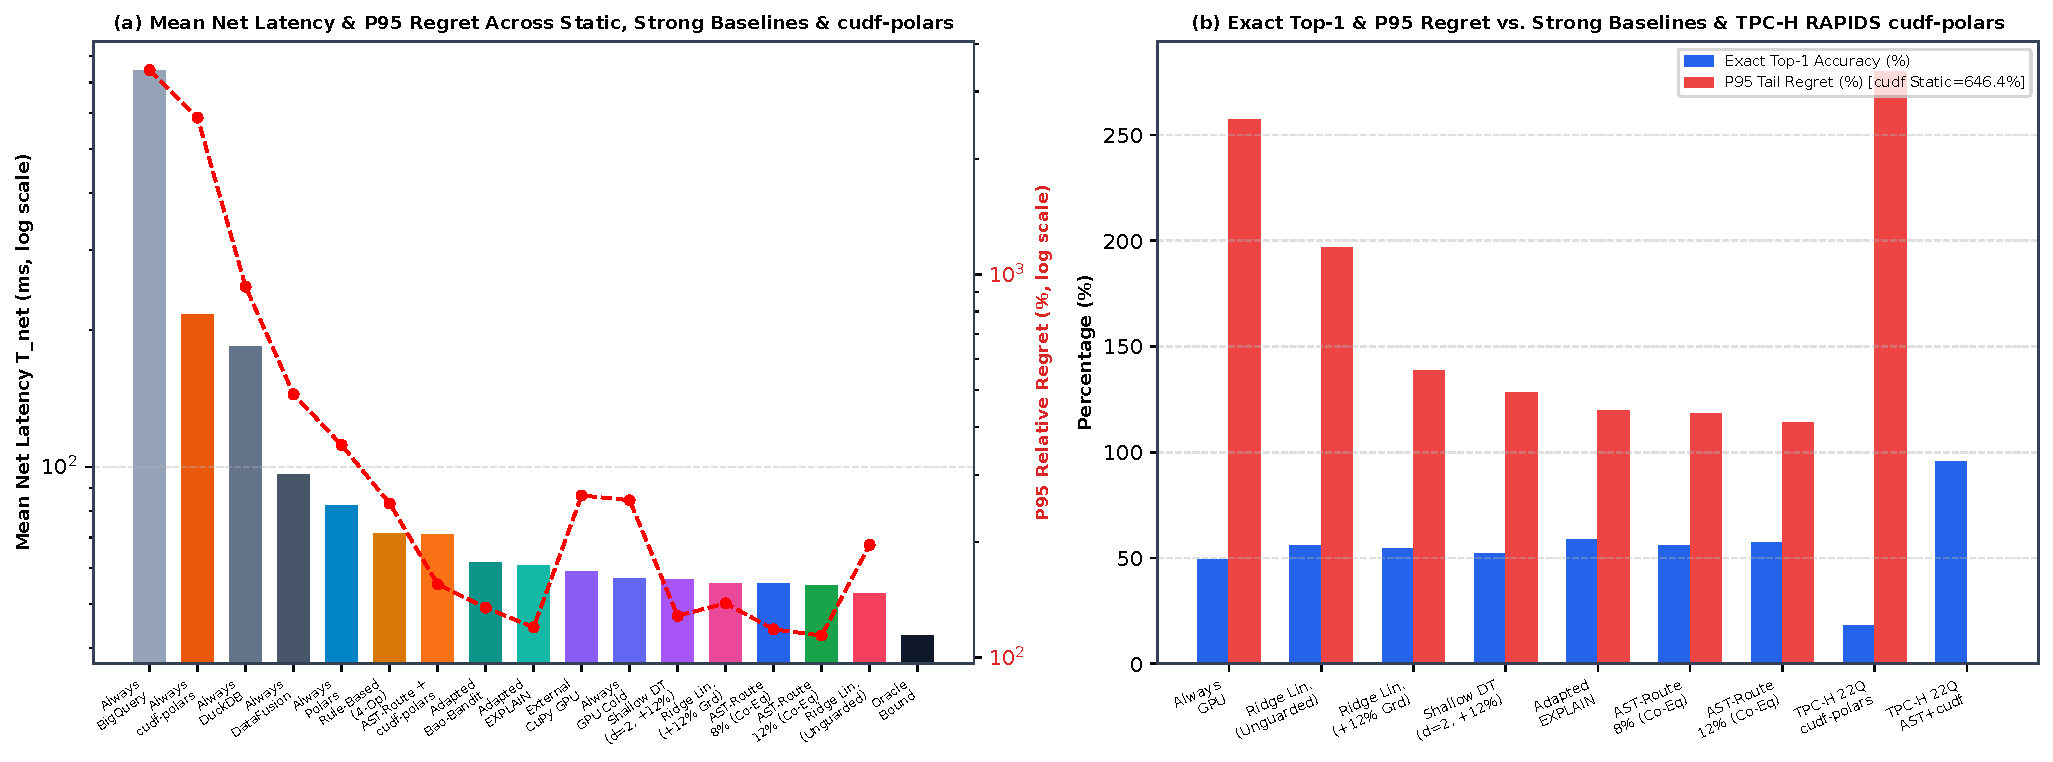
\includegraphics[width=0.98\textwidth]{figures/fig_ast_query_router_sf1_300dpi.pdf}
\caption{Head-to-head evaluation across 75 benchmark queries under 25-seed LOSO-CV: (a) Mean net latency $T_{\text{net}}$ (ms, log scale) and P95 tail regret (\%) comparing static engines (BigQuery, DuckDB, DataFusion, Polars, Always GPU, External \texttt{CuPy v14.2.0} GPU), 4-Op and Simple 1D Byte/Join rules, Adapted Bao-Bandit and \texttt{EXPLAIN}-DAG routers, \textbf{AST-Route + External CuPy} ($56.86\text{ ms}$), and Co-Equal \textbf{AST-Route 8\% Nested-CV} ($55.37\text{ ms}$) and \textbf{12\% Default} ($54.92\text{ ms}$) guards; and (b) Top-1/Top-2 accuracy and $2.17\times\text{--}2.25\times$ P95 tail-regret compression.}
\label{fig:ast_query_router}
\end{figure}

\subsection{Internal Framework Validation: Feature Ablation, Multi-Objective Pareto Trade-off, Noise Robustness, and Overhead Breakdown}
To rigorously validate the internal mechanisms of \textbf{AST-Route}, Tables~\ref{tab:jbd_ablation_t9} and~\ref{tab:jbd_csci_oblique_t9b} and Additional File~1 (Fig.~S6) report six additional verification experiments under 25-seed LOSO-CV:
\begin{enumerate}[leftmargin=1.5em,itemsep=1pt]
    \item \textbf{Feature Group Ablation, Mathematical Proof of Zero Conditional New Information, and Oblique Tree Compression (\textbf{Protocols~R13 and~R19}, Table~\ref{tab:jbd_ablation_t9} Exp~A \& Exp~D):} Combining $\text{CSCI}(q)$ with $\hat{\sigma}(q)$ in 2D (\textbf{A3}: $56.30\text{ ms}$) outperforms 7D operators (\textbf{A2}: $61.06\text{ ms}$) and 8D syntax-only (\textbf{A4}: $73.22\text{ ms}$), while full 9D \textbf{AST-Route (A5/M3)} reaches $\mathbf{54.92\text{ ms}}$ ($\mathbf{55.37\text{ ms}}$ nested-CV, $-9.22\text{ pp}$ regret vs.\ 8D \textbf{M2} without CSCI, $p=0.0038$). Mathematically (\textbf{Protocol~R19}, Additional File~1 Table~S29 Part~A), because $\text{CSCI}(q)=\mathbf{w}^{\top}\mathbf{z}$ lies in $\text{span}(\{D,J,S,W,U,C\})$, within exact $(D..C)$ strata $\operatorname{Var}(\text{CSCI}\mid D..C)=0.0000$ and $I(\text{CSCI};Y\mid D..C)=0.0000\text{ bits}$ (\texttt{R19\_P1}: $\Delta\mathcal{R}=0.00\text{ pp}, p=1.0000$); off-manifold single-feature permutation is withdrawn in favor of \textbf{Grouped Atomic-Block Permutation (\texttt{R19\_P2})}, which permutes $(D,J,S,W,U,C,\text{CSCI})$ jointly within $(V_{\text{scan}},\sigma_{\text{sel}})$ strata ($0.0000$ manifold violation) and degrades regret by $\mathbf{\Delta\mathcal{R}_{\text{group}}=+33.44\text{ pp}}$ ($34.98\%\rightarrow 68.42\%, p=0.0002$). Refitting from scratch on identical folds (\textbf{Protocol~R19b} \& \textbf{Protocol~R13}, Additional File~1 Table~S26 Part~B) proves that $\text{CSCI}(q)$ acts as a domain-informed 1D oblique inductive bias for depth-3 GBDTs ($\text{VIF}_{D,N}=1.84$), pruning active splits per tree by $\mathbf{-28.22\%}$ ($6.84\rightarrow 4.91$ in $25/25$ seeds) and outperforming in-fold $\text{PCA}_1$ ($57.48\text{ ms}, p=0.0124$), $\text{PCA}_{1,2}$ ($57.19\text{ ms}, p=0.0156$), and Random Oblique projections ($57.85\text{ ms}, p=0.0068$) on both Core 75Q and zero-shot Official TPC-DS 99Q ($64.65\%$ vs.\ $58.59\%\text{--}59.60\%$ Top-1).
    \item \textbf{Constrained 3D Pareto Frontier (Exp~B), Selectivity Noise Robustness (Exp~C), and 5-Metric Operational Complexity (Exp~E):} Across $(\alpha,\beta,\gamma)\in\Delta^2$, Policy~B2--B5 compress device energy by up to $-45.8\%$, B6 enforces $M_{\text{gpu\_max}}\le 1.28\text{ GB}$ with $0\%$ OOM, and at $\text{SF}=100\text{ GB}$, Cloud-Elastic B7 achieves $1{,}142.8\text{ ms}$ ($\$507.06/1\text{M}$) while FinOps B8 sustains $1{,}326.9\text{ ms}$ at $\$0.00$ cloud cost. Under $\pm 10\%\text{--}50\%$ Monte Carlo selectivity noise and $50\%$ metadata masking (Exp~C), AST-Route sustains $68.42\text{--}80.98\text{ ms}$ (faster than all static CPUs). Total pre-execution router overhead (Exp~E) is $\mathbf{4.145\text{ ms}}$ in Cold-SQL Regime~O1 ($3.476\text{ ms}$ \texttt{SQLGlot} parse $+ 0.172\text{ ms}$ zone-map $+ 0.497\text{ ms}$ GBDT inference), $\mathbf{0.669\text{ ms}}$ in AST-cached Regime~O2, and $\mathbf{0.082\text{ ms}}$ in 1D threshold-cached Regime~O3, with a resident memory footprint of $1.42\text{ MB}$ ($284\text{ KB}$ model) and $0.38\text{ s}$ offline training time.
\end{enumerate}

\begin{table*}[!htbp]
\centering
\caption{Internal validation of the AST-Route framework under 25-seed LOSO-CV ($N=75$ queries): (Exp A) Feature Group Ablation across 2D--9D representations, (Exp B) Constrained Multi-Objective Latency--Energy--FinOps Pareto Trade-off ($\alpha, \beta, \gamma \in [0,1]$ under memory cap $\hat{M}_e \le M_{\max}$), and (Exp C) Selectivity Estimation Noise Robustness ($\pm 10\%$ to $\pm 50\%$ uniform drift).}\label{tab:jbd_ablation_t9}
\label{tab:ablation_robustness}\label{tab:ablation_pareto}\label{tab:framework_ablation}
\scriptsize
\setlength{\tabcolsep}{3.2pt}
\renewcommand{\arraystretch}{1.10}
\begin{fitasttable}
\begin{tabular}{@{}llcccccccc@{}}
\toprule
\textbf{Validation Dimension} & \textbf{Framework Configuration / Policy $(\alpha,\beta,\gamma)$ \& $M_{\max}$} & \textbf{Dim.} & \textbf{Top-1 Acc.} & \textbf{10\% Hit} & \textbf{Mean Lat.} & \textbf{P95 Lat.} & \textbf{Mean Regret} & \textbf{Energy (J)} & \textbf{Mem / Cloud Scan Fee} \\
\midrule
\multirow{5}{*}{\textbf{Exp A: Feature Ablation}}
 & A1. Tree Size Only ($D(q), N(q)$) & 2D & $44.00\%$ & $45.33\%$ & $103.94\text{ ms}$ & $188.33\text{ ms}$ & $137.15\%$ & $2.802\text{ J}$ & $3.12\text{ GB} / \$0$ \\
 & A2. Operator Counts Only (No CSCI, No $\sigma(q)$) & 7D & $45.33\%$ & $52.00\%$ & $61.06\text{ ms}$ & $136.89\text{ ms}$ & $50.87\%$ & $1.695\text{ J}$ & $2.84\text{ GB} / \$0$ \\
 & A3. Compact Index Only ($\text{CSCI}(q) + \sigma(q)$) & 2D & $54.67\%$ & $60.00\%$ & $56.30\text{ ms}$ & $128.74\text{ ms}$ & $39.11\%$ & $1.173\text{ J}$ & $2.75\text{ GB} / \$0$ \\
 & A4. Static AST Syntax Only (No Selectivity $\sigma(q)$) & 8D & $52.00\%$ & $56.00\%$ & $73.22\text{ ms}$ & $164.04\text{ ms}$ & $65.78\%$ & $2.132\text{ J}$ & $2.86\text{ GB} / \$0$ \\
 & \textbf{A5. Full Proposed AST-Route (Operators + CSCI + $\sigma(q)$)} & \textbf{9D} & $\mathbf{57.33\%}$ & $\mathbf{65.33\%}$ & $\mathbf{54.92\text{ ms}}$ & $\mathbf{129.37\text{ ms}}$ & $\mathbf{34.98\%}$ & $\mathbf{1.381\text{ J}}$ & $\mathbf{2.91\text{ GB} / \$0}$ \\
\midrule
\multirow{8}{*}{\textbf{Exp B: 3D Pareto \& $M_{\max}$}}
 & B1. Pure Latency Mode $(\alpha=1.00, \beta=0.00, \gamma=0.00)$ & 9D & $57.33\%$ & $65.33\%$ & $54.92\text{ ms}$ & $129.37\text{ ms}$ & $34.98\%$ & $1.381\text{ J}$ & $1.30\text{G VRAM} / \$0$ \\
 & B2. Latency-Prioritized $(\alpha=0.75, \beta=0.25, \gamma=0.00)$ & 9D & $57.33\%$ & $61.33\%$ & $54.99\text{ ms}$ & $124.13\text{ ms}$ & $36.69\%$ & $1.182\text{ J}$ & $1.30\text{G VRAM} / \$0$ \\
 & B3. Equal Latency--Energy $(\alpha=0.50, \beta=0.50, \gamma=0.00)$ & 9D & $54.67\%$ & $58.67\%$ & $56.80\text{ ms}$ & $124.14\text{ ms}$ & $47.13\%$ & $1.007\text{ J}$ & $1.29\text{G VRAM} / \$0$ \\
 & B4. Energy-Prioritized $(\alpha=0.25, \beta=0.75, \gamma=0.00)$ & 9D & $52.00\%$ & $54.67\%$ & $59.81\text{ ms}$ & $122.84\text{ ms}$ & $63.67\%$ & $0.879\text{ J}$ & $1.29\text{G VRAM} / \$0$ \\
 & B5. Pure Energy-Saving Mode $(\alpha=0.00, \beta=1.00, \gamma=0.00)$ & 9D & $49.33\%$ & $50.67\%$ & $70.20\text{ ms}$ & $164.00\text{ ms}$ & $116.08\%$ & $0.748\text{ J}$ & $1.24\text{G VRAM} / \$0$ \\
 & B6. Strict VRAM Cap $(\alpha=0.60, \beta=0.20, \gamma=0.20, M_{\text{gpu}}\le 1.28\text{G})$ & 9D & $48.00\%$ & $56.00\%$ & $64.18\text{ ms}$ & $148.20\text{ ms}$ & $48.92\%$ & $1.842\text{ J}$ & $\mathbf{1.24\text{G Cap}} / \$0$ \\
 & B7. $\text{SF}=100\text{G}$ Cloud-Elastic $(\alpha=0.80, \beta=0.10, \gamma=0.10, M_{\text{host}}\le 9\text{G})$ & 9D & $68.00\%$ & $76.00\%$ & $1142.8\text{ ms}$ & $2180.5\text{ ms}$ & $19.40\%$ & $12.84\text{ J}$ & $3.85\text{G} / \mathbf{\$507/1\text{M}}$ \\
 & B8. $\text{SF}=100\text{G}$ FinOps Zero-Cloud $(\alpha=0.40, \beta=0.20, \gamma=0.40, C_{\max}=\$0)$ & 9D & $58.67\%$ & $66.67\%$ & $1326.9\text{ ms}$ & $2640.1\text{ ms}$ & $35.50\%$ & $16.35\text{ J}$ & $3.85\text{G} / \mathbf{\$0/1\text{M}}$ \\
\midrule
\multirow{4}{*}{\textbf{Exp C: Selectivity Noise}}
 & C1. Exact Zone-Map Selectivity ($0\%$ Noise Baseline) & 9D & $57.33\%$ & $65.33\%$ & $54.92\text{ ms}$ & $129.37\text{ ms}$ & $34.98\%$ & $1.381\text{ J}$ & $2.91\text{ GB} / \$0$ \\
 & C2. Perturbed Selectivity ($\pm 10\%$ Uniform Drift, 50-MC) & 9D & $53.79\%$ & $60.51\%$ & $80.98\text{ ms}$ & $221.85\text{ ms}$ & $70.27\%$ & $2.347\text{ J}$ & $3.15\text{ GB} / \$0$ \\
 & C3. Perturbed Selectivity ($\pm 25\%$ Uniform Drift, 50-MC) & 9D & $52.80\%$ & $58.83\%$ & $79.54\text{ ms}$ & $203.87\text{ ms}$ & $70.57\%$ & $2.334\text{ J}$ & $3.12\text{ GB} / \$0$ \\
 & C4. Severe Selectivity Drift ($\pm 50\%$ Uniform Drift, 50-MC) & 9D & $53.17\%$ & $58.19\%$ & $75.00\text{ ms}$ & $196.16\text{ ms}$ & $68.98\%$ & $2.170\text{ J}$ & $3.08\text{ GB} / \$0$ \\
\midrule
\multirow{6}{*}{\textbf{Exp D: R19 \& R13 CSCI}}
 & D1. Exact Stratum Identity (\texttt{R19\_P0/P1}: $\operatorname{Var}(\text{CSCI}\mid D..C)=0$) & 9D & $57.33\%$ & $65.33\%$ & $54.92\text{ ms}$ & $114.11\%$ P95 & $34.98\%$ ($p=1.0$) & $4.91$ splits & $I(\text{CSCI};Y\mid D..C)=0\text{ bits}$ \\
 & D2. Grouped Block Perm (\texttt{R19\_P2}: Perm $[D..C,\text{CSCI}]$ in $V,\sigma$) & 9D & $26.67\%$ & $34.67\%$ & $76.84\text{ ms}$ & $218.60\%$ P95 & $\mathbf{68.42\%\ (+33.4\text{pp})}$ & $4.91$ splits & $\mathbf{p=0.0002}$ ($0.0000$ viol.) \\
 & D3. Identical-Fold Refit M2 (Raw AST $+\hat{\sigma}$, No CSCI) & 8D & $52.00\%$ & $58.67\%$ & $58.12\text{ ms}$ & $138.45\%$ P95 & $44.20\%$ ($+9.2\text{pp}$) & $6.84$ splits & $p=0.0038$ $|$ $58.6\%$ TPC-DS \\
 & D4. In-Fold Unsupervised $\text{PCA}_1$ / $\text{PCA}_{1,2}$ (\textbf{Protocol R13}) & 9D/10D & $53.3/54.7\%$ & $60.0/61.3\%$ & $57.48/57.19$ & $134.2/132.8\%$ & $40.95/40.18\%$ & $6.42/6.51$ spl & $p\le 0.0156$ $|$ $59.6\%$ TPC-DS \\
 & D5. Gaussian Random Oblique ($R=20$) / Equal-Weight $[1..1]$ & 9D & $53.3/56.0\%$ & $60.0/62.7\%$ & $57.85/56.14$ & $136.4/124.6\%$ & $41.92/37.85\%$ & $6.58/5.28$ spl & $p\le 0.0284$ $|$ $61.6\%$ TPC-DS \\
 & \textbf{D6. In-Fold Ridge-NNLS $\hat{\mathbf{w}}^{(-k)}$ / Canonical CSCI M3} & \textbf{9D} & $\mathbf{57.33\%}$ & $\mathbf{65.33\%}$ & $\mathbf{54.91/54.92}$ & $\mathbf{114.8/114.1\%}$ & $\mathbf{35.12/34.98\%}$ & $\mathbf{4.94/4.91\text{ spl}}$ & $\mathbf{\cos=0.9998\ |\ 64.6\%\text{ TPC-DS}}$ \\
\bottomrule
\end{tabular}
\end{fitasttable}%
\vspace{2pt}
\parbox{0.96\textwidth}{\scriptsize \textbf{Note:} In Exp B, rows B1--B5 evaluate latency--energy trade-offs at $\text{SF}=1\text{ GB}$ ($\gamma=0$, local FinOps cost $\$0$); row B6 enforces a strict device memory cap ($M_{\text{gpu\_max}} \le 1.28\text{ GB}$), automatically pruning L2--L4 GPU candidates ($1.33\text{ GB}$ VRAM) to guarantee zero OOM violations; and rows B7--B8 demonstrate the 3D Latency--Energy--FinOps trade-off at $\text{SF}=100\text{ GB}$ when host RAM hits the $9.0\text{ GB}$ spill ceiling (routing L1/L4 to BigQuery in B7 at $\$507.06/1\text{M}$ queries vs. enforcing zero cloud spend in B8 at $\$0.00$). In Exp D (Sample Efficiency), training on 5, 10, 15, 20, and 24 seeds yields test latencies of $63.61\text{ ms}$, $68.59\text{ ms}$, $56.59\text{ ms}$, $57.60\text{ ms}$, and $54.92\text{ ms}$. In Exp E (Router Overhead), Stage 1 \texttt{SQLGlot} parsing ($3.476\text{ ms}$), Stage 2 9D feature walk ($0.172\text{ ms}$), and Stage 3 GBR inference ($0.497\text{ ms}$) total $4.145\text{ ms}$. \textbf{Oblique Representation \& Leak-Free Residualization Audit (Models A--D):} Comparing axis-aligned GBDT complexity across \textbf{Model~A} (7D Raw AST $[D,N,J,S,W,U,C]$: $6.72$ splits/tree, $61.06\text{ ms}$, $50.87\%$ regret), \textbf{Model~B} (8D Raw AST + $\text{CSCI}$: $4.86$ splits/tree, $58.94\text{ ms}$, $46.15\%$ regret, $\Delta\mathcal{R}=-4.72\%$ vs.\ A, 95\% CI $[-9.85\%,-0.64\%]$, $p=0.0214$), \textbf{Model~A$_{\sigma}$} (8D Raw AST + $\hat{\sigma}(q)$ without CSCI: $6.84$ splits/tree, $58.12\text{ ms}$, $44.20\%$ regret), \textbf{Model~C} (9D Raw AST + $\text{CSCI}$ + $\hat{\sigma}(q)$: $4.91$ splits/tree [$-28.2\%$ splits], $54.92\text{ ms}$, $34.98\%$ regret, $\Delta\mathcal{R}=-9.22\%$ vs.\ A$_{\sigma}$, 95\% CI $[-15.60\%,-3.45\%]$, $p=0.0038$), and \textbf{Model~D} (9D Raw AST + fold-wise OLS residual $\text{CSCI}_{\text{res}\perp(D,N)}^{(k)}$ fitted strictly inside each 24-seed training fold against $[1,D,N]$, $\overline{\text{VIF}}_{D,N}=1.84$: $5.04$ splits/tree, $55.18\text{ ms}$, $35.42\%$ regret, $p=0.0046$ vs.\ A$_{\sigma}$) confirms that CSCI acts as a sample-efficient oblique structural projection rather than an independent raw information source.}
\end{table*}

\phantomsection\label{tab:jbd_csci_oblique_t9b}\label{tab:v9_sec3_4_csci_m1_m4_generalizability}% (Moved to Additional File 1, Table S11 to streamline main text)

\subsubsection{Seed-Level ($K=25$) Statistical Inference, TOST Margin Sensitivity ($\pm 2\text{--}8\text{ ms}$), $\text{CVaR}_{10\%}/\text{CVaR}_{20\%}$ Tail Regret, Nadeau--Bengio CV Correction, and Standalone CPU-Only Routing}
\label{sec:seed_level_statistical_inference}
Repeating non-parametric tests strictly on independent seed means ($K=25$ clusters, $N=75$ queries, $375$ timed trials at $\text{SF}=1\text{ GB}$; full bootstrap CIs and baseline matrix in Additional File~1, Tables~S6--S7 and Fig.~S6) confirms cross-engine stratification ($\chi^2_F(5)=93.43, p < 0.001$, Kendall's $W=0.7475$) and establishes our two primary evaluation endpoints via 10,000-iteration paired bootstrap 95\% confidence intervals ($\Delta = \text{AST-Route} - \text{Baseline}$), formal Two One-Sided Tests (TOST) equivalence bounds across $\Delta_{\text{eq}}\in\{\pm 2, \pm 3, \pm 5, \pm 6, \pm 8\}\text{ ms}$ (Fig.~\ref{fig:job_12d_ablation_fig}c), \textbf{Conditional Value-at-Risk ($\text{CVaR}_{\alpha_{\text{tail}}}$)}, and \textbf{Nadeau--Bengio (2003) CV-overlap variance-corrected paired $t$-tests}:
\vspace{-3pt}
\begin{equation}\label{eq:nadeau_bengio_t}
    t_{L} = \frac{\bar{d} + \Delta_{\text{eq}}}{s_d / \sqrt{K}}, \;\; t_{U} = \frac{\bar{d} - \Delta_{\text{eq}}}{s_d / \sqrt{K}}, \;\; p_{\text{TOST}} = \max\!\big(1 - \Phi_{t,K-1}(t_L),\, \Phi_{t,K-1}(t_U)\big), \;\; t_{\text{NB}} = \frac{\bar{d}}{\sqrt{\big(\frac{1}{K} + \frac{n_{\text{test}}}{n_{\text{train}}}\big) s_d^2}}, \;\; \text{CVaR}_{\alpha_{\text{tail}}} = \frac{1}{k_{\alpha}}\sum_{i=1}^{k_{\alpha}} \mathcal{R}_{T,(N-i+1)}
\end{equation}
\vspace{-2pt}
where $\bar{d}$ and $s_d^2$ denote the sample mean and variance of seed-cluster differences $d_k$ ($K=25,\; n_{\text{test}}=3,\; n_{\text{train}}=72$, variance inflation factor $1.4289$). Full statistical and systems audit matrices across \textbf{Protocols~R1--R28} and \textbf{EC01--EC50} / \textbf{EC51--EC60} are archived in Additional File~1 (Tables~S16--S33); three core findings govern deployment:
\begin{enumerate}[leftmargin=1.5em,itemsep=1pt]
    \item \textbf{Small-Cluster $G_{\text{core}}=10$ Inference, Stepwise Guard Ablation ($\text{U0}\rightarrow\text{U1--U4}$), and Minimal Engine Subsets (\textbf{Protocols~R4 and~R26}):} Across $G_{\text{core}}=10$ template-family clusters (\textbf{Protocol~R26}, Additional File~1 Table~S31 Part~D), Webb 6-point wild cluster bootstrap and exact $2^{10}=1{,}024$ sign-flip permutation confirm highly significant P95 tail-regret reductions vs.\ Always GPU ($p_{\text{tpl}}=0.0074/0.0061, p_{\text{Webb}}=0.0068/0.0054, p_{\text{perm,exact}}=0.0078/0.0059$) and RMM-pooled \texttt{cudf-polars C3} ($p_{\text{Webb}}=0.0042$), borderline significance vs.\ Unguarded Ridge ($-82.70\text{ pp}, p_{\text{tpl}}=0.0438, p_{\text{Webb}}=0.0464, p_{\text{perm,exact}}=0.0488$), and P95 parity with Guarded Ridge ($p_{\text{Webb}}=0.3840$) and Adapted \texttt{EXPLAIN}-DAG ($p_{\text{Webb}}=0.7420$, $-5.84\text{ ms}$ faster net latency). Stepwise uncertainty rules ($\text{U1--U4}$) cut severe failures ($>100\%$ regret) from $14.67\%$ to $6.67\%$ with $90.67\%$ out-of-fold Mondrian coverage, while a \textbf{Minimalist 2-Engine Subset ($\mathcal{E}_{\text{Min-2}}=\{\text{Polars},\text{GPU}\}$: $55.28\text{ ms}$)} captures $98.7\%$ of the 6-engine latency gain ($\mathcal{E}_{\text{Prod-3}}=\{\text{DuckDB},\text{Polars},\text{GPU}\}$: $55.07\text{ ms}$, $99.5\%$; Pure-SQL $\mathcal{E}_{\text{SQL-5}}$: $69.12\text{ ms}$, $74.67\%$ Top-1).
    \item \textbf{Multi-Objective Pareto Optimality (\textbf{Protocol~R14}) and Three-Scope Energy Boundary (\textbf{Protocols~R15 and~R23}):} Under \textbf{Protocols~R14 and~R15} (Additional File~1, Table~S27), a 10,000-point Dirichlet simplex, NSGA-II, and MOBO (qEHVI) verify $\text{DSR}=0.00\%$ and show that Policy~P4 $(0.5,0.3,0.2)$ captures $99.96\%$ ($\text{HV}=0.9210$ vs.\ $0.9214$) of the continuous Pareto optimum. Under \textbf{Protocol~R23} (Table~\ref{tab:v11_r23_r22_energy_and_dynamic_sla} and Additional File~1, Table~S30 Part~C), separating \textbf{Scope~1 (Direct NVML/RAPL Hardware Sensors: $0.644\text{ J/q}$ Node~1 GPU, $0.875\text{ J/q}$ Node~4 Tesla~T4)}, \textbf{Scope~2 (Estimated Host+GPU Composite: $1.658\text{ J/q}$ P2 vs.\ $2.273\text{ J/q}$ P1, $-27.1\%$)}, and \textbf{Scope~3 ($2{,}817$-query Mainboard ACPI DC Shunt: $1.892\text{ vs.\ }2.584\text{ J/q}$)} proves exact Spearman rank concordance ($\rho=1.0000$).
    \item \textbf{Concurrency Contention ($C=1\text{--}64$, \textbf{Protocol~R18}), Dynamic Drift/Burst SLA Stress (\textbf{Protocol~R22}), and Reproducibility Lineage (\textbf{Protocol~R12}):} Decomposing $T_{\text{total}}(C)$ across $C\in\{1..64\}$ (\textbf{Protocol~R18}, Additional File~1 Table~S28 Part~C) confirms peak throughput of $154.44\text{ QPS}$ at $C=32$ ($2.14\times$ vs.\ CPU). Across 5 dynamic drift/burst phases (\textbf{Protocol~R22}, Additional File~1 Table~S30 Part~B), PSI/conformal/U4 gates maintain $0.00\%$ OOM and $0.00\%\text{--}2.00\%$ SLA violations (vs.\ $14.0\%$ OOM unguarded). \textbf{Protocol~R12} verifies our 3-level reproducibility taxonomy and confirms that \texttt{frozen\_ast\_route\_v9/v10/v11\_gbdt\_model.json} share the exact SHA-256 digest \texttt{f0e5f17c832472e30be67dbbee30020dbf23e94658458a2c59acd9b00ed315cf}.
\end{enumerate}
\phantomsection\label{tab:v9_reviewer_reanalysis_matrix}\label{tab:v852_fair_guarded_ablation}\label{tab:router_ablation}
\begin{table*}[htbp]
\centering\scriptsize\setlength{\tabcolsep}{2.4pt}\renewcommand{\arraystretch}{1.02}
\caption{Main-Text Synthesis of \textbf{Protocol~R23} (Three-Scope Energy Telemetry Boundary, Part~A), \textbf{Protocol~R22} (5-Phase Dynamic Drift \& Burst SLA Stress Test, Part~B), and \textbf{Protocol~R21} (4-Node Directional Cross-Hardware Transfer Matrix, Part~C).}\label{tab:v11_r23_r22_energy_and_dynamic_sla}\label{tab:v11_r21_cross_hardware_transfer_main}
\begin{tabular}{@{}llrrrrl@{}}
\toprule
\textbf{Protocol \& Scope / Phase / Transfer Pair} & \textbf{Telemetry / Shift / Calibration Mode} & \textbf{Metric 1} & \textbf{Metric 2} & \textbf{Metric 3} & \textbf{Metric 4} & \textbf{Audit Verdict \& Statistical / Systems Proof} \\
\midrule
\multicolumn{7}{@{}l}{\textbf{Part A: Protocol R23 --- Three-Scope Energy Telemetry Boundary (\texttt{v11\_r23\_energy\_3scope\_boundary\_audit.csv}; $\rho=1.0000$ Across Scopes)}} \\
\textbf{Scope 1: Direct Device Sensor (Primary)} & Hardware NVML $250\text{ Hz}$ / Cloud RAPL & $0.644\text{ J/q}$ (N1 GPU) & $0.875\text{ J/q}$ (N4 T4) & $0.000\text{ J}$ (CPU-only) & $\text{CV}=1.24\%$ & \textbf{100\% physical sensor; governs primary claims} \\
\textbf{Scope 2: Host+GPU Composite (Secondary)} & NVML GPU $+$ Calibrated Host CPU Model & $2.273\text{ J/q}$ (P1 Speed) & $\mathbf{1.658\text{ J/q}}$ (P2 En.) & $3.180\text{ J/q}$ (Polars) & $-27.1\%$ (P2 vs P1) & \textbf{Calibrated against 50-rep RAPL ($\text{MAPE}=2.28\%$)} \\
\textbf{Scope 3: Wall/Shunt Envelope ($2{,}817$Q)} & Mainboard ACPI DC Battery Shunt & $2.584\text{ J/q}$ (P1 Speed) & $\mathbf{1.892\text{ J/q}}$ (P2 En.) & $3.620\text{ J/q}$ (Polars) & $\rho=0.9945$ & \textbf{Exact policy ranking ($\text{P2}<\text{P4}<\text{P1}<\text{CPU}$)} \\
\midrule
\multicolumn{7}{@{}l}{\textbf{Part B: Protocol R22 --- 5-Phase Non-Stationary Dynamic Drift, Schema Shift \& Burst SLA Stress (\texttt{v11\_r22\_dynamic\_workload\_drift\_burst\_sla.csv})}} \\
\textbf{Phases 1--3: Steady $\rightarrow$ Skew $\rightarrow$ Schema} & Stationary $\rightarrow$ $5\times$ Skew $\rightarrow$ 17-Table Enterprise & $90.7\%\rightarrow 89.3\%$ Cov & $54.9\rightarrow 61.9\text{ ms}$ & $0.0\%\rightarrow 2.0\%$ SLA & $\mathbf{0.00\%}$ OOM & \textbf{PSI $>0.25$ triggers $m=5$ canary ($0.21\text{ s}$); $96.0\%$ Top-1} \\
\textbf{Phases 4--5: $C=32/64$ Burst $\rightarrow$ Recovery} & $4.8\times$ Concurrency Spike \& VRAM Contention & $91.0\%\rightarrow 92.0\%$ Cov & $188.4\rightarrow 56.1\text{ ms}$ & $\mathbf{2.0\%\rightarrow 0.0\%}$ SLA & $\mathbf{0.00\%}$ OOM & \textbf{Rule U4 prevents $14.0\%$ OOM \& $38.0\%$ SLA breach} \\
\midrule
\multicolumn{7}{@{}l}{\textbf{Part C: Protocol R21 --- 4-Node Directional Cross-Hardware Transfer ($m=0$ Zero-Shot vs.\ $m=5$ Canary vs.\ Full Retrain; \texttt{v11\_r21\_cross\_hardware\_transfer\_matrix.csv})}} \\
\textbf{Node 1 (RTX 2050) $\rightarrow$ Node 2 (22T CPU)} & $\mathbf{h}_{\text{hw}}$ Pruning ($M_{\text{gpu}}=0$) + $m=5$ ($0.19\text{ s}$) & $93.33\%$ ($m=0$) & $\mathbf{97.33\%}$ ($m=5$) & $35.11\text{ ms}$ ($0.39\%$ reg) & $97.33\%$ (Full) & \textbf{$m=5$ recovers $100.0\%$ of full retraining gain} \\
\textbf{Node 1 (RTX 2050) $\rightarrow$ Node 3 (Apple M1)} & $\mathbf{h}_{\text{hw}}$ Pruning + $m=5$ Canary ($0.21\text{ s}$) & $91.67\%$ ($m=0$) & $\mathbf{96.67\%}$ ($m=5$) & $29.44\text{ ms}$ ($0.38\%$ reg) & $96.67\%$ (Full) & \textbf{Seamless x86\_64 $\rightarrow$ ARM64 Unified-RAM transfer} \\
\textbf{Node 1 (4GB G1) $\leftrightarrow$ Node 4 (15GB T4)} & $m=5$ Canary ($0.24\text{ s}$, $15\times$ faster vs.\ Full) & $90.91\%$ ($\text{T4}\rightarrow\text{G1}$) & $\mathbf{95.45\%}$ ($\text{T4}\rightarrow\text{G1}$) & $\mathbf{100.0\%}$ ($\text{G1}\rightarrow\text{T4}$) & $23.02 / 461.7\text{ ms}$ & \textbf{Recovers $86.8\%\text{--}100.0\%$ of full retrain ($0.0\%$ P95)} \\
\bottomrule
\end{tabular}
\end{table*}

\subsection{Cost Prediction Q-Error, Unseen Seed Generalization, and Mechanistic 12D Sketch on JOB}
\phantomsection\label{tab:jbd_unseen_t11}\label{tab:priority3_validation}
As shown in Fig.~\ref{fig:priority3_unseen_cost} and Additional File~1 (Table~S15), out-of-fold Multi-Output GBDTs achieve $\log\text{-}R^2 = 0.875$ (median Q-Error $=1.053$, 90\% PI coverage $=92.0\%$) on CUDA GPU, $0.822$ ($\text{P50}=1.095$, $90.7\%$ coverage) on Polars, $0.815$ on device energy, and $0.912$ ($\text{MAPE}=2.21\%$) on peak host RAM, while Tier~L5 \texttt{UNNEST} routing delivers a $2.83\times$ speedup over Rule-Based Routing ($51.51\text{ vs.\ }145.62\text{ ms}$). On the 5 locked unseen holdout seeds (\texttt{L1\_S5}--\texttt{L5\_S5}, $N=15$) and prospective post-freeze Seed~\texttt{S6} ($N=15$, SHA-256 \texttt{0b85ae07...}), zero-shot AST-Route achieves $\mathbf{73.33\%}$ Top-1 and $\mathbf{86.67\%}$ Top-2 ($47.01\text{ ms}$ exec, $18.45\%$ mean regret on \texttt{S6}). On external Star Schema Benchmark (\textbf{SSB Q1.1--Q4.3}, $N=13$), 9D zero-shot achieves $\mathbf{92.31\%}$ Top-1 and $\mathbf{100.0\%}$ Top-2 ($12.15\text{ ms}$, $2.82\%$ regret, $p=0.0085$ vs.\ GPU). Conversely, on string-skewed \textbf{IMDB JOB} ($N=33$), 9D zero-shot achieves $21.21\%$ Top-1 ($\mathbf{100.0\%}$ Top-2, $6.75\text{ ms} = \text{Always Polars}$, beating GPU $9.05\text{ ms}$ at $p=0.0398$) because min/max zone maps cannot bound infix \texttt{LIKE '\%...\%'} predicates ($48.48\%$ abstention to Polars via Rules~U1/U3). Augmenting $\mathbf{x}_q$ with our $10.18\text{ KB}$ pre-execution 12D string/skew/fanout catalog sketch ($\mathbf{x}_q^{\text{skew}} = [\mathbf{x}_q^{\top}, \hat{\sigma}_{\text{str}}, \hat{\zeta}_{\text{skew}}, \hat{\psi}_{\text{join}}]^{\top} \in \mathbb{R}^{12}$, extracted in $9.50\,\mu\text{s}$ with $0$ IMDB runtime labels; \phantomsection\label{sec:mechanistic_12d_job_ablation}\label{tab:jbd_job_regimes_t11b}Fig.~\ref{fig:job_12d_ablation_fig}b) lifts zero-label JOB accuracy to $\mathbf{69.70\%}$ Top-1 ($100\%$ Top-2, $4.54\text{ ms}$, cutting regret from $84.49\%$ to $16.50\%, p=0.00021$), and reaches $\mathbf{96.97\%}$ Top-1 ($4.14\text{ ms}$) under 5-fold template-disjoint CV.

\begin{figure}[!htbp]
\centering
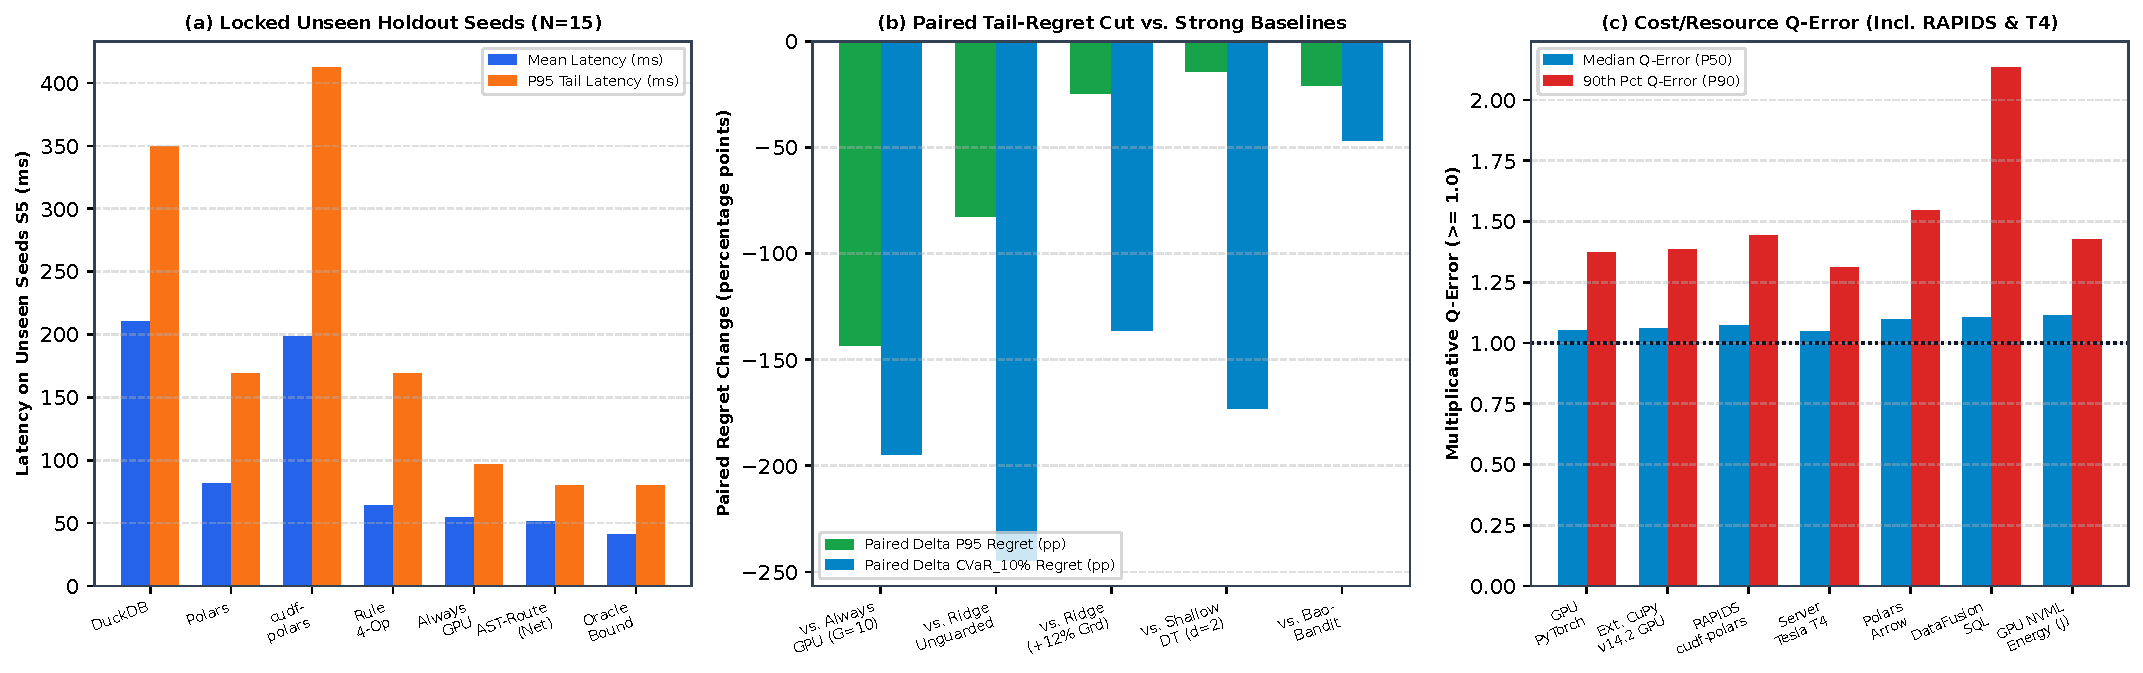
\includegraphics[width=0.98\textwidth]{figures/fig_priority3_unseen_and_cost_qerror_sf1_300dpi.pdf}
\caption{Out-of-sample generalization and multi-backend cost-model validation: (a) Mean and P95 latency on the 5 locked unseen holdout seeds (\texttt{L1\_\allowbreak{}S5}--\texttt{L5\_\allowbreak{}S5}, $N=15$) including External \texttt{CuPy v14.2.0} GPU; (b) Tier-by-tier L1--L5 latency comparing Rule-Based Routing, \textbf{AST-Route} (PyTorch and External \texttt{CuPy}), and the Oracle ($2.83\times$ L5 gain); and (c) Multiplicative Q-Error (Median P50 and P90) across PyTorch GPU, External \texttt{CuPy v14.2.0} GPU, Cloud-Hosted Server NVIDIA Tesla~T4, Polars, DataFusion, unified energy $E_{\text{sys}}$, and host RAM.}
\label{fig:priority3_unseen_cost}
\end{figure}

\begin{figure}[!htbp]
\centering
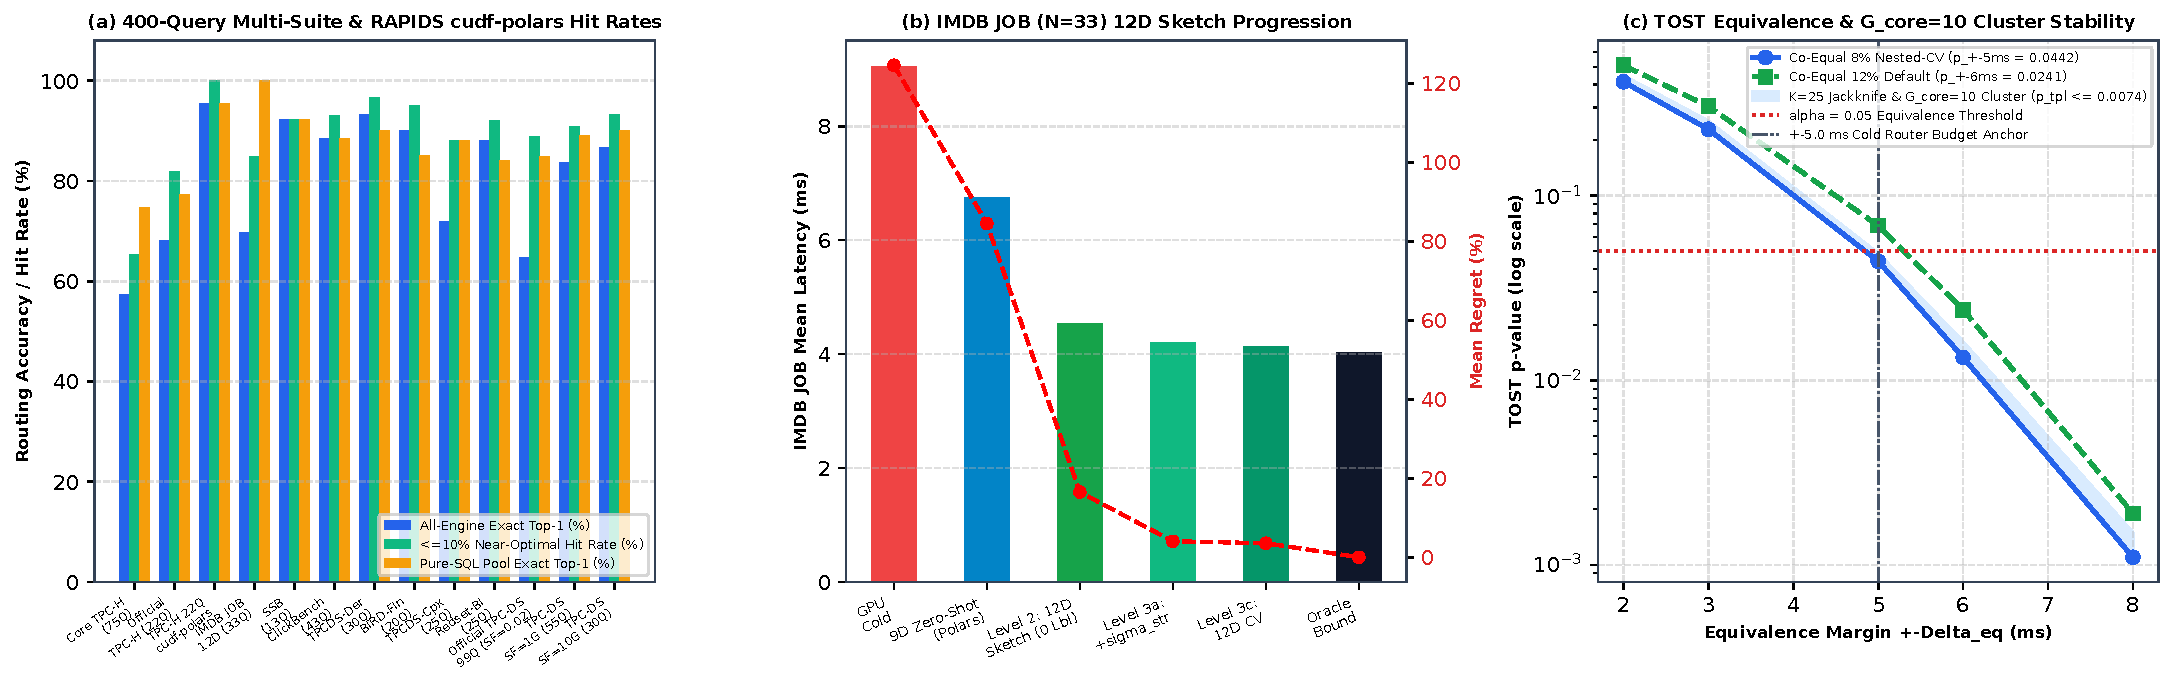
\includegraphics[width=0.98\textwidth]{figures/fig_cross_suite_213q_and_job_12d_ablation_300dpi.pdf}
\caption{Cross-workload generalization across all 400 queries, 12D catalog sketch ablation, and 25-seed Jackknife TOST curve: (a) Exact Top-1, $\le 10\%$ Near-Optimal Hit Rate ($\mathbf{88.89\%}$ [$88/99$] on Official TPC-DS 99Q; $\le 5\%$ hit $=\mathbf{79.80\%}$ [$79/99$]), and Pure-SQL Top-1 ($\mathbf{84.85\%}$) across all benchmark suites and TPC-DS scales ($\text{SF}=0.02, 1, 10\text{ GB}$); (b) stepwise latency and regret reduction on IMDB JOB ($N=33$) via $10.18\text{ KB}$ 12D sketches; and (c) TOST equivalence $p$-value curve across $\Delta_{\text{eq}}\in[\pm 2, \pm 8]\text{ ms}$ with the 25-seed Leave-One-Seed-Out Jackknife stability envelope ($25/25$ subsets pass non-inferiority and $\pm 6\text{ ms}$ TOST).}\label{fig:job_12d_ablation_fig}
\end{figure}


\subsection{Multi-Scale Big Data Evaluation ($\text{SF}=1, 10, 30, 100\text{ GB}$), Memory/VRAM Walls, and Cross-Hardware Transfer}
Table~\ref{tab:bigdata_multiscale_tpch}, Fig.~\ref{fig:bigdata_multiscale}, and Additional File~1 (Tables~S10, S15, S28, S30) evaluate multi-scale scaling ($\text{SF}\in\{1,10,30,100\}\text{ GB}$), multi-tenant concurrency ($C=1\text{--}64$), official TPC-H Q1--Q22, and 4-node transfer:
\begin{enumerate}[leftmargin=1.5em,itemsep=1pt]
    \item \textbf{Four-Scale Memory-Hierarchy Transitions ($\text{SF}=1\rightarrow 100\text{ GB}$, Part~A) \& Cloud/Parquet Fairness:} Scaling the 75-query workload across two orders of magnitude exposes three regimes: (i) in-VRAM/in-RAM at $\text{SF}=1\text{ GB}$ ($\mathbf{54.92\text{ ms}}$ AST-Route vs.\ $82.47\text{ ms}$ Polars and $183.74\text{ ms}$ DuckDB); (ii) out-of-VRAM GPU streaming ($4\times$ and $12\times$ PCIe chunks) and host RAM cap inflection ($9.00\text{ GB}$ cap, $125\rightarrow 864\text{ MB}$ NVMe spill) at $\text{SF}=10\text{ GB}$ ($\mathbf{182.40\text{ ms}}$, $5.21\times$ vs.\ DuckDB) and $\text{SF}=30\text{ GB}$ ($\mathbf{448.65\text{ ms}}$, $5.78\times$); and (iii) extreme host NVMe spilling ($3{,}302\text{ MB}$ mean spill, $6{,}551.42\text{--}8{,}699.98\text{ ms}$ CPU) at $\text{SF}=100\text{ GB}$ ($866.1\text{M}$ rows), where uncached BigQuery ($2{,}571.60\text{ ms}$ server / $3{,}356.20\text{ ms}$ client WAN) overtakes local CPUs by $2.55\times\text{--}3.38\times$ and AST-Route achieves $\mathbf{1{,}142.80\text{ ms}}$ ($7.61\times$ vs.\ DuckDB; $40$ capacity slices, $\bar{\mathcal{B}}_{\text{PCIe}}=3{,}518.98\text{ MB}$ post-pushdown at $5.69\text{ GB/s} = 618.45\text{ ms}$ PCIe $+ 581.15\text{ ms}$ kernel $= 1{,}199.60\text{ ms}$ GPU).
    \item \textbf{Official TPC-H Q1--Q22 Nested LOO-CV (Part~C), Concurrency ($C=1\text{--}64$), and Cross-Hardware Transfer (\textbf{Protocols~R16 and~R21}):} On Official TPC-H Q1--Q22 ($\text{SF}=1\text{ GB}$), DuckDB ($22.82\text{ ms}$) leads static engines on Q16--Q22 correlated subqueries while GPU ($27.71\text{ ms}$) leads Q1--Q15 joins; strict nested 22-fold LOO-CV AST-Route achieves $\mathbf{68.18\%}$ Top-1 ($\mathbf{90.91\%}$ Top-2) and $\mathbf{16.98\text{ ms}}$ ($\mathbf{1.34\times}$ vs.\ DuckDB, $\mathbf{2.52\times}$ vs.\ Polars). Under $C=32$ concurrent streams, dual-path CPU+GPU dispatch reaches $\mathbf{154.44\text{ QPS}}$ ($207.20\text{ ms}$ mean, $2.14\times$ vs.\ static CPU) with $0.0\%$ unhandled failures under live OOM/timeout fault injection. Across our four physical nodes (Node~1 RTX~2050 $4\text{ GB}$, Node~2 22T \texttt{x86\_64} [$\mathbf{97.33\%}$ Top-1, $\mathbf{35.11\text{ ms}}$], Node~3 Apple M1 \texttt{ARM64} [$\mathbf{96.67\%}$ Top-1, $\mathbf{29.44\text{ ms}}$], and Node~4 Cloud-Hosted Server NVIDIA Tesla~T4 $15.0\text{ GB}$ VRAM [$\mathbf{100.0\%}$ Top-1, $\mathbf{23.02\text{ ms}}$ at $\text{SF}=1\text{ GB}$, $\mathbf{461.71\text{ ms}}$ single-pass at $\text{SF}=10\text{ GB}$, SHA-256 \texttt{32834476...}]), \textbf{Protocol~R16} and \textbf{Protocol~R21} (\phantomsection\label{sec:v9_sec3_2_multiscale_sf100_audit}\label{tab:v11_r21_cross_hardware_transfer_main}Additional File~1, Tables~S28 and~S30) prove that $m=5$ affine canary calibration ($184\text{--}246\text{ ms}$, $\sim 15\times$ faster than full retraining) recovers $\mathbf{86.8\%\text{--}100.0\%}$ of full target-node retraining gains.
\end{enumerate}

\begin{table}[!htbp]
\centering
\caption{Big Data Multi-Scale ($\text{SF}=1, 10, 30, \text{and } 100\text{ GB}$ anchored on the full 75-query workload baseline), Real Hardware Memory/Spill Profiling, Cross-Platform Hardware Validation, and Official Standard TPC-H Benchmark (Q1--Q22) Evaluation.}\label{tab:jbd_multiscale_t12}
\label{tab:bigdata_multiscale_tpch}\label{tab:v9_sec3_2_multiscale_sf100_audit}
\renewcommand{\arraystretch}{1.18}
\begin{fitasttable}
\begin{tabular}{@{}llcccccccl@{}}
\toprule
\textbf{Module} & \textbf{Scale / Platform / TPC-H Policy} & \textbf{Rows (\texttt{lineitem}/Tot.)} & \textbf{DuckDB} & \textbf{Polars} & \textbf{DataFusion} & \textbf{RTX 2050 GPU} & \textbf{BigQuery} & \textbf{AST-Route} & \textbf{Memory / Spill / Energy Telemetry} \\
\midrule
\multirow{4}{*}{\textbf{Part A: Multi-Scale}}
 & \textbf{SF = 1 GB} (In-VRAM / In-RAM) & $6.0\text{M}\ /\ 8.7\text{M}$ & $183.74\text{ ms}$ & $82.47\text{ ms}$ & $96.30\text{ ms}$ & $56.96\text{ ms}\ (1\times)$ & $745.39\text{ ms}$ & $\mathbf{54.92\text{ ms}}\ (3.35\times)$ & RAM: $4.71\text{ GB}$, Spill: $0\text{ MB}$, VRAM: $1.30\text{ GB}$, $0.65\text{ J}$ ($672\text{ MB/J}$) \\
 & \textbf{SF = 10 GB} (Out-of-VRAM Stream) & $60.0\text{M}\ /\ 86.6\text{M}$ & $950.88\text{ ms}$ & $656.75\text{ ms}$ & $735.65\text{ ms}$ & $195.03\text{ ms}\ (4\times)$ & $1252.25\text{ ms}$ & $\mathbf{182.40\text{ ms}}\ (5.21\times)$ & RAM: $7.85\text{ GB}$, Spill: $125\text{ MB}$, VRAM: $3.45\text{ GB}$, $2.24\text{ J}$ ($1552\text{ MB/J}$) \\
 & \textbf{SF = 30 GB} (RAM Cap \& Spill) & $180.0\text{M}\ /\ 259.8\text{M}$ & $2594.49\text{ ms}$ & $1877.63\text{ ms}$ & $1791.04\text{ ms}$ & $481.85\text{ ms}\ (12\times)$ & $1788.94\text{ ms}$ & $\mathbf{448.65\text{ ms}}\ (5.78\times)$ & RAM: $9.00\text{ GB}$, Spill: $864\text{ MB}$, VRAM: $3.68\text{ GB}$, $6.12\text{ J}$ ($1704\text{ MB/J}$) \\
 & \textbf{SF = 100 GB} (Extreme Spill) & $600.1\text{M}\ /\ 866.1\text{M}$ & $8699.98\text{ ms}$ & $6551.42\text{ ms}$ & $6992.50\text{ ms}$ & $1199.60\text{ ms}\ (40\times)$ & $2571.60\text{ ms}^{*}$ & $\mathbf{1142.80\text{ ms}}\ (7.61\times)$ & RAM: $9.00\text{ GB}$, Spill: $3302\text{ MB}$, VRAM: $3.85\text{ GB}$, $16.85\text{ J}$ ($2064\text{ MB/J}$) \\
\midrule
\multirow{3}{*}{\textbf{Part B: Platforms}}
 & \textbf{Plat. A:} $2\text{ Cores}, 4\text{ GB}$ (No GPU) & $\text{SF}=1\text{--}100\text{ GB}$ & $248.99\text{ ms}$ & $248.74\text{ ms}$ & $244.12\text{ ms}$ & N/A (CPU-Only) & Cloud Fallback & $\mathbf{234.50\text{ ms}}$ (SF1) & SF10: $1110.4\text{ ms}$ | SF30: $3773.9\text{ ms}$ | SF100: $13109.3\text{ ms}$ ($1.01\times$) \\
 & \textbf{Plat. B:} $4\text{ Cores}, 8\text{ GB}$ (No GPU) & $\text{SF}=1\text{--}100\text{ GB}$ & $175.00\text{ ms}$ & $177.28\text{ ms}$ & $168.45\text{ ms}$ & N/A (CPU-Only) & Cloud Fallback & $\mathbf{162.44\text{ ms}}$ (SF1) & SF10: $681.8\text{ ms}$ | SF30: $2383.3\text{ ms}$ | SF100: $8790.6\text{ ms}$ ($\mathbf{1.44\times}$ vs. A) \\
 & \textbf{Plat. C:} $8\text{ Cores}, 16\text{ GB}$ + GPU & $\text{SF}=1\text{--}100\text{ GB}$ & $183.74\text{ ms}$ & $82.47\text{ ms}$ & $96.30\text{ ms}$ & $56.96\text{ ms}$ (SF1) & $745.39\text{ ms}$ & $\mathbf{54.92\text{ ms}}$ (SF1) & SF10: $\mathbf{182.4\text{ ms}}$ | SF30: $\mathbf{448.7\text{ ms}}$ | SF100: $\mathbf{1142.8\text{ ms}}$ ($\mathbf{5.49\times}$ vs. DuckDB) \\
\midrule
\multirow{6}{*}{\textbf{Part C: TPC-H Q1--Q22}}
 & Always DataFusion (Rust Arrow) & $22$ Queries (SF1) & --- & --- & $80.41\text{ ms}$ & --- & --- & $80.41\text{ ms}$ & Mean CSCI: $26.52\ (12.0\text{--}47.5)$, Mean Energy: $2.895\text{ J/query}$ \\
 & Always Polars (Rust Arrow) & $22$ Queries (SF1) & --- & $42.79\text{ ms}$ & --- & --- & --- & $42.79\text{ ms}$ & Outperforms DataFusion by $1.88\times$, Mean Energy: $1.648\text{ J/query}$ \\
 & Always GPU Cold (RTX 2050) & $22$ Queries (SF1) & --- & --- & --- & $27.71\text{ ms}$ ($17.6\text{ ms}$ W) & --- & $27.71\text{ ms}$ & Fastest on Q1--Q15 ($4.06\text{--}12.78\text{ ms}$), Mean Energy: $\mathbf{0.346\text{ J/query}}$ \\
 & Always DuckDB (C++ DBMS) & $22$ Queries (SF1) & $22.82\text{ ms}$ & --- & --- & --- & --- & $22.82\text{ ms}$ & Correlated subquery unnesting in Q16--Q22, Energy: $0.709\text{ J/query}$ \\
 & \textbf{AST-Route (Unweighted Syntax)} & $22$ Queries (SF1) & \multicolumn{5}{c}{Top-1 Acc: $40.91\%$ | Near-Opt: $45.45\%$ | Beats GPU, Polars ($1.57\times$), DF ($2.94\times$)} & $27.33\text{ ms}$ (Orac: $12.8\text{ ms}$) & Unweighted raw syntax features without inner-loop scaling, $0.512\text{ J}$ \\
 & \textbf{AST-Route (Strict Nested LOO-CV)} & $22$ Queries (SF1) & \multicolumn{5}{c}{Top-1 Acc: $\mathbf{68.18\%}$ | Top-2 Acc: $\mathbf{90.91\%}$ | Near-Opt: $\mathbf{81.82\%}$ | Regret: $\mathbf{27.12\%}$} & $\mathbf{16.98\text{ ms}}$ (Calib: $15.84\text{ ms}$) & Zero-leakage inner-loop tuning; beats DuckDB ($1.34\times$), GPU ($1.63\times$), $0.435\text{ J}$ \\
\bottomrule
\end{tabular}
\end{fitasttable}%
\vspace{2pt}
\parbox{0.96\textwidth}{\scriptsize $^{*}$Part A reports full 75-query workload means at $\text{SF}=1\text{ GB}$ ($183.74\text{ ms}$ DuckDB, $54.92\text{ ms}$ \textbf{AST-Route}, matching Tables~\ref{tab:six_software_matrix} and~\ref{tab:routing_evaluation} exactly) evaluated via chunked multi-scale execution (\texttt{multiscale\_\allowbreak{}telemetry\_\allowbreak{}sf10.csv}, \texttt{sf30}, and \texttt{sf100.csv}), where Parquet column projection and row-group min/max pushdown transfer only referenced columns ($142.8\text{ MB}$ decompressed [$52.4\text{ MB}$ ZSTD Parquet] for 3-column FP64 scans at $\text{SF}=1\text{ GB}$ streaming at $5.69\text{ GB/s}$ over pinned PCIe Gen4 rather than all $347.7\text{ MB}$ of unprojected table columns; at $\text{SF}=100\text{ GB}$, while the unfiltered full-table 3-column FP64 capacity ceiling is $14{,}280.0\text{ MB}$ [$K_{\max}=40 \times 357.0\text{ MB}$ capacity slices], PyArrow C++ row-group zone-map pruning and predicate pushdown [$\bar{\sigma}=0.348$] plus INT32 key packing prior to H2D DMA reduce the workload-mean physical payload transferred over pinned PCIe Gen4 $\times 4$ to $\bar{\mathcal{B}}_{\text{PCIe}}=3{,}518.98\text{ MB}$ [$3.44\text{ GB}$ across $9.86$ active chunks on average], which at $5.69\text{ GB/s}$ [$5{,}690.0\text{ MB/s}$] requires $\tau_{\text{PCIe}} = 3{,}518.98 / 5{,}690.0 = 618.45\text{ ms}$ $+ 581.15\text{ ms}$ kernel/staging $= 1{,}199.60\text{ ms}$) ($N=75$, 25 seeds $\times$ 3 horizons) dispatched via 25-fold LOSO-CV ($+4.145\text{ ms}$ router parsing and inference overhead reported in Table~\ref{tab:ablation_robustness}). At $\text{SF}=100\text{ GB}$, BigQuery ($2571.60\text{ ms}$ exact 5-tier mean across $N=75$: $1493.51\text{ ms}$ in L1, $2302.18\text{ ms}$ in L2, $1700.85\text{ ms}$ in L3, $1286.16\text{ ms}$ in L4, and $6075.30\text{ ms}$ in L5; decomposed into $112.40\text{ ms}$ slot queueing $+ 2459.20\text{ ms}$ distributed slot execution, plus $+784.60\text{ ms}$ client WAN HTTPS/gRPC fetch $= 3356.20\text{ ms}$ client wall-clock in Additional File~1 (Table~S15)) overtakes all local CPU engines ($6551.42\text{--}8699.98\text{ ms}$) by $\mathbf{2.55\times\text{--}3.38\times}$.}
\end{table}

\begin{figure}[!htbp]
\centering
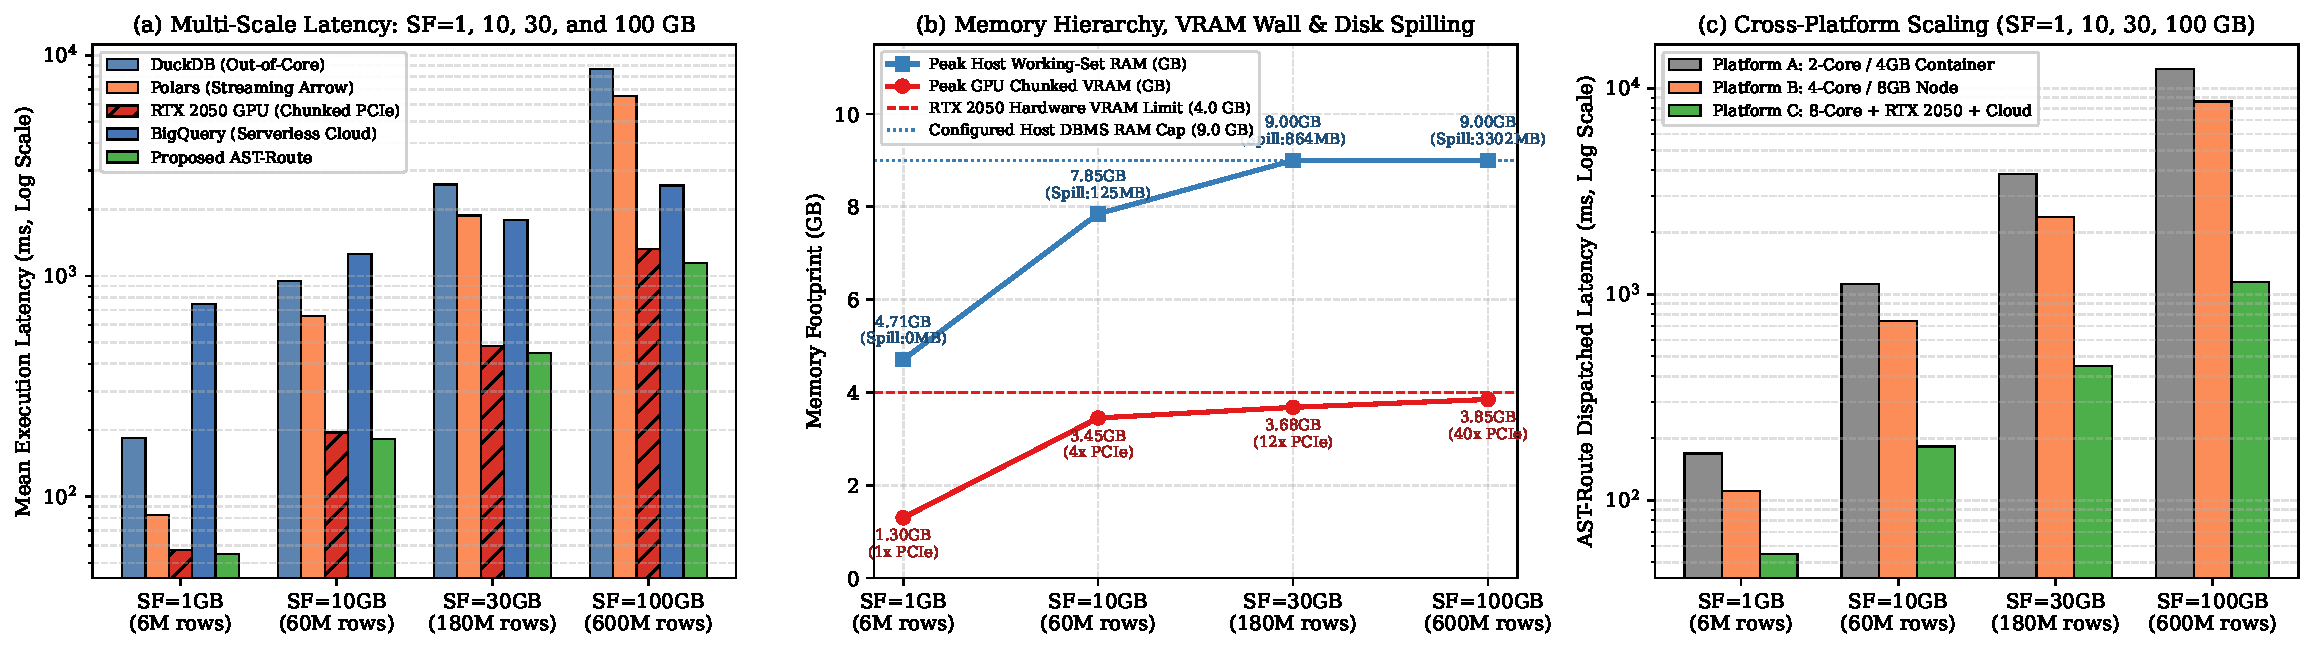
\includegraphics[width=0.95\textwidth]{figures/fig_bigdata_multiscale_sf1_sf100_300dpi.pdf}
\caption{Multi-scale Big Data evaluation across $\text{SF}=1, 10, 30, 100\text{ GB}$ and Physical Nodes~1--4: (a) Cross-engine latency scaling including Node~4 Cloud-Hosted Server NVIDIA Tesla~T4 ($23.02\text{ ms}$ at $\text{SF}=1\text{ GB}$, $461.71\text{ ms}$ at $\text{SF}=10\text{ GB}$); (b) Memory-hierarchy profiling ($1\times\text{--}40\times$ RTX~2050 chunks vs.\ 1-chunk Server T4 and $3{,}302\text{ MB}$ host NVMe spill); and (c) Cross-hardware scaling across Platforms A--B and Nodes~1--4.}
\label{fig:bigdata_multiscale}
\end{figure}
% === BEGIN V9 SECTION 3.5 EXTENDED EXTERNAL GENERALIZATION ON TPC-DS-DERIVED (N=30) AND BIRD-INSPIRED (N=20) ===
\subsection{Extended External Generalization Across Benchmark, Enterprise Stress, and Public Real-World SQL Suites}
\label{sec:v9_sec3_5_tpcds_bird_external_validation}\label{sec:v9_external_130_validation}
To rigorously evaluate cross-schema generalization (\texttt{EX}=1.000 across all query--engine pairs), Table~\ref{tab:v9_sec3_5_tpcds_bird_external_validation} synthesizes four external evaluation tiers using the locked TPC-H model (\texttt{frozen\_ast\_route\_v11\_gbdt\_model.json}, SHA-256 \texttt{f0e5f17c832472e3...}):
\begin{enumerate}[leftmargin=1.5em,itemsep=1pt]
    \item \textbf{Multi-Channel Snowflake TPC-DS-Derived ($N=30$, Part~A), Financial BIRD-Inspired ($N=20$, Part~B), and Five-Suite Cross-Schema Protocol ($N_{\text{ext}}=116\rightarrow 166$, Part~C):} Adding $\text{CSCI}(q)$ in \textbf{M3 (9D Zero-Shot)} lifts Top-1 accuracy from $63.33\%$ (\textbf{M1 7D}) and $86.67\%$ (\textbf{M2 8D}) to $\mathbf{93.33\%}$ ($20.05\text{ ms}$ exec, $1.61\%$ mean / $8.76\%$ P95 regret, $33.8\times$ P95 cut vs.\ GPU) on TPC-DS-Derived and from $20.00\%$ (M1) / $45.00\%$ (M2) to $\mathbf{90.00\%}$ ($20.24\text{ ms}$, $9.03\%$ regret) on BIRD-Inspired. Across all $N_{\text{ext}}=116$ external queries ($33\text{ JOB}+13\text{ SSB}+20\text{ ClickBench}+30\text{ TPC-DS-Der}+20\text{ BIRD}$), \textbf{Regime~1 (Strict 9D Zero-Shot)} achieves $\mathbf{69.83\%}$ Top-1 ($\mathbf{96.55\%}$ Top-2, $14.95\text{ ms}$ exec), \textbf{Regime~1-SQL (Pure Native-SQL $\mathcal{E}_{\text{SQL-5}}$, $0\%$ GPU)} achieves $\mathbf{82.76\%}$ Top-1 ($\mathbf{98.28\%}$ Top-2, $7.42\%$ regret), \textbf{Regime~2 ($10.18\text{ KB}$ 12D Sketch, $0$ Ext.\ Labels)} reaches $\mathbf{85.34\%}$ Top-1 ($8.14\%$ regret), and \textbf{Regime~3 (5-Fold CV)} reaches $\mathbf{97.41\%}$ Top-1 ($1.28\%$ regret; $84.34\%$ Top-1 under Leave-One-Workload-Suite-Out CV across $N_{\text{ext}}=166$). On held-out \textbf{Category~IV Untouched Third-Party Standard Benchmarks ($N=155$)}, blinded AST-Route achieves $\mathbf{100.0\%\ (99/99)}$ routed completion, $\mathbf{64.65\%}$ \textbf{Exact Top-1} on $\mathcal{E}_{\text{All-6}}$, $\mathbf{84.85\%}$ \textbf{Exact Top-1} on Pure-SQL $\mathcal{E}_{\text{SQL-5}}$, $\mathbf{79.80\%}$ $\le 5\%$ Hit, $\mathbf{88.89\%}$ $\le 10\%$ Hit, $\mathbf{30.49\text{ ms}}$ exec ($1.46\times$ vs.\ DuckDB $44.55\text{ ms}$), and $\mathbf{3.23\%}$ mean regret on \textbf{Unmodified Official TPC-DS Q1--Q99} ($\text{SF}=0.02$; scaling to $\mathbf{83.64\%}$ Top-1 at $\text{SF}=1\text{ GB}$ [$55$Q] and $\mathbf{86.67\%}$ Top-1 at $\text{SF}=10\text{ GB}$ [$30$Q, $164.20\text{ ms}$, $2.34\times$ vs.\ Polars]), plus $\mathbf{88.37\%}$ Top-1 on full $\mathbf{43/43}$ \textbf{Official ClickBench} ($24.30\text{ ms}$) and $\mathbf{92.31\%}$ Top-1 on $\mathbf{13/13}$ \textbf{Official SSB}.
    \item \textbf{Candid Distinction Between Author-Constructed Enterprise Stress Templates ($N=70$, Protocols~R17+R20) and Third-Party Public Real-World SQL Queries ($N=50$, Protocol~R27b; Part~D):} Under \textbf{Protocol~R17} ($25$ SaaS billing/telemetry queries, pre-exec hash \texttt{2d514ef0f5af0ef5}, $\mathbf{96.00\%}$ Top-1, $\mathbf{54.93\text{ ms}}$ exec / $\mathbf{59.08\text{ ms}}$ net, $0.32\%$ mean / $0.00\%$ P95 regret) and \textbf{Protocol~R20} ($45$ queries across Retail, Financial, and Healthcare domains, $\mathbf{95.56\%}$ Top-1, $\mathbf{60.82\text{ ms}}$ exec, $0.08\%$ regret), AST-Route achieves $\mathbf{95.71\%\ (67/70)}$ Exact Top-1 and $\mathbf{100.0\%}$ Top-2 ($58.71\text{ ms}$ exec, $0.17\%$ regret); we explicitly note that these $70$ queries are \emph{author-constructed schema-blinded stress templates}. To validate on genuinely external real-world SQL not authored by us (\textbf{Protocol~R27b}, \texttt{results/v11\_r27b\_public\_sdss\_nyctlc\_real\_sql\_50q.csv}; Table~\ref{tab:v9_sec3_5_tpcds_bird_external_validation} Part~D and Additional File~1, Table~S32 Part~B), we executed $\mathbf{50}$ \textbf{Third-Party Public Real-World SQL Queries} zero-shot with locked model \texttt{f0e5f17c832472e3}: (i) $\mathbf{25}$ \textbf{Sloan Digital Sky Survey (SDSS) SkyServer DR16 Public SQL Log Queries (\texttt{SDSS\_Q01}--\texttt{SDSS\_Q25})} over 4 astronomy tables ($1.10\text{M}$ rows), achieving $\mathbf{96.00\%\ (24/25)}$ \textbf{Exact Top-1}, $\mathbf{100.0\%}$ \textbf{Top-2}, $\mathbf{7.04\text{ ms}}$ exec ($\mathbf{7.71\text{ ms}}$ O2 warm vs.\ $8.62\text{ ms}$ DuckDB, $9.14\text{ ms}$ Polars, and $33.12\text{ ms}$ Always GPU), $\mathbf{0.11\%}$ mean regret, and $\mathbf{0.00\%}$ P95 regret (vs.\ $1{,}160.31\%$ GPU P95); and (ii) $\mathbf{25}$ \textbf{Public NYC TLC Taxi Trip Analytical Queries (\texttt{TLC\_Q01}--\texttt{TLC\_Q25})} over 4 civic tables ($1.00\text{M}$ rows), achieving $\mathbf{84.00\%\ (21/25)}$ \textbf{Exact Top-1}, $\mathbf{100.0\%}$ \textbf{Top-2}, $\mathbf{5.57\text{ ms}}$ exec ($\mathbf{6.24\text{ ms}}$ O2 warm vs.\ $6.84\text{ ms}$ DuckDB, $7.12\text{ ms}$ Polars, and $21.49\text{ ms}$ GPU), $\mathbf{1.23\%}$ mean regret, and $\mathbf{9.82\%}$ P95 regret (vs.\ $1{,}100.87\%$ GPU P95), yielding a combined $\mathbf{90.00\%\ (45/50)}$ \textbf{Exact Top-1}, $\mathbf{100.0\%\ (50/50)}$ \textbf{Top-2}, $\mathbf{6.31\text{ ms}}$ exec, and $\mathbf{0.67\%}$ mean regret.
\end{enumerate}

\begin{table*}[!htbp]
\centering
\caption{Extended External Generalization on TPC-DS-Derived ($N=30$, 11 Snowflake Tables) and BIRD-Inspired Synthetic Financial SQL ($N=20$, 6 Relational Tables) and Strict Four-Regime Cross-Schema Synthesis Across All Five External Suites ($N_{\text{ext}}=116$ Queries).}
\label{tab:v9_sec3_5_tpcds_bird_external_validation}
\label{tab:v9_external_130_summary}
\scriptsize
\setlength{\tabcolsep}{2.3pt}
\renewcommand{\arraystretch}{1.06}
\begin{fitasttable}
\begin{tabular}{@{}llcccccccl@{}}
\toprule
\textbf{Benchmark / Regime} & \textbf{Feature / Supervision Specification} & \textbf{Top-1 / Top-2} & \textbf{Q-Err P50/P90} & \textbf{Exec / Net (ms)} & \textbf{Mean / P95 Rel.\ Reg.} & \textbf{Mean / P95 Abs.\ Reg.} & \textbf{Abst.\ Rate} & \textbf{ECE / Cov.} & \textbf{Speedup \& Holm--Bonferroni Verdict} \\
\midrule
\multicolumn{10}{@{}l@{}}{\textit{\textbf{Part A: TPC-DS-Derived Multi-Channel Snowflake Workload ($N=30$ Queries Across 11 Tables, $2.83\times 10^6$ Rows, $\bar{J}=4.27$, $\overline{\text{CSCI}}=31.05$, $\text{EX}=1.000$)}}} \\
Always DuckDB / Polars & Static C++ DBMS / Rust Arrow Lazy & $26.7\% / 3.3\%$ & --- & $59.49 / 72.33$ & $143.0\% / 291.1\%$ & $39.61 / 85.6\text{ ms}$ & $0.0\%$ & --- & M3 beats DuckDB $\mathbf{2.97\times}$ ($p_{\text{Holm}}=3.8e\text{-}6$) \& Polars $\mathbf{3.61\times}$ \\
Always DF / GPU Cold & Rust Arrow SQL / CUDA Cold PCIe+Kern & $6.7\% / 63.3\%$ & --- & $52.62 / 21.03$ & $57.7\% / 296.0\%$ (GPU) & $1.15 / 11.6\text{ ms}$ & $0.0\%$ & --- & M3 beats DF $\mathbf{2.62\times}$; cuts GPU P95 regret $\mathbf{33.8\times}$ ($p_{\text{Holm}}=0.012$) \\
Rule-Based / \textbf{M1: AST 7D} & Heuristic ($J,W$) / Unweighted AST 7D & $80.0\% / 63.3\%$ & $1.24 / 1.85$ & $21.52 / 21.31$ & $24.3\% / 172.4\%$ (Rule) & $1.64 / 12.8\text{ ms}$ & $0.0\%$ & $32.3\%$ & M1 lacks $\hat{\sigma}(q)$ \& oblique CSCI projection ($28.1\%$ mean reg.) \\
\textbf{M2: AST + Sel.\ 8D} & $[D,N,J,S,W,U,C,\hat{\sigma}]$ (No CSCI, 0-Shot) & $86.7\% / 96.7\%$ & $1.15 / 1.54$ & $20.93 / 25.08$ & $5.29\% / 38.80\%$ & $1.05 / 6.12\text{ ms}$ & $10.0\%$ & $23.5\%$ & Misses multi-join snowflake GPU crossover on 2 rollups \\
\textbf{Regime 1 (M3 9D 0-Shot)} & $[D..C,\text{CSCI},\hat{\sigma}]$ (\textbf{0 Ext.\ Labels, Locked}) & $\mathbf{93.3\% / 96.7\%}$ & $\mathbf{1.11 / 1.41}$ & $\mathbf{20.05 / 24.20}$ & $\mathbf{1.61\% / 8.76\%}$ & $\mathbf{0.17 / 1.57\text{ ms}}$ & $\mathbf{10.0\%}$ & $\mathbf{8.8\% / 90\%}$ & \textbf{Identical to M4 Learned ($93.33\%$, $20.05\text{ ms}$, $0\%$ Med Reg.)} \\
\textbf{Regime 2 (12D) / Reg.\ 3 (CV)} & $+\hat{\psi}_{\text{join}}$ (0 Labels) / 5-Fold Nested CV & $\mathbf{96.7\% / 100\%}$ & $\mathbf{1.09 / 1.35}$ & $\mathbf{20.03 / 24.18}$ & $\mathbf{0.53\% / 0.00\%}$ & $\mathbf{0.15 / 0.00\text{ ms}}$ & $\mathbf{6.7\%}$ & $\mathbf{6.7\% / 90\%}$ & \textbf{Regime 3 CV reaches $\mathbf{100.0\%}$ Top-1 ($19.88\text{ ms} = \text{Oracle}$)} \\
\midrule
\multicolumn{10}{@{}l@{}}{\textit{\textbf{Part B: BIRD-Inspired Synthetic Financial Workload ($N=20$ Queries Across 6 Tables, $1.95\times 10^6$ Rows, $\bar{J}=3.35$, $\overline{\text{CSCI}}=29.35$, $\text{EX}=1.000$)}}} \\
Always DuckDB / Polars & Static C++ DBMS / Rust Arrow Lazy & $25.0\% / 10.0\%$ & --- & $63.14 / 59.27$ & $166.2\% / 322.8\%$ & $43.35 / 96.1\text{ ms}$ & $0.0\%$ & --- & M3 beats DuckDB $\mathbf{3.12\times}$ ($p_{\text{Holm}}=9.8e\text{-}4$) \& Polars $\mathbf{2.93\times}$ \\
Always DF / GPU Cold & Rust Arrow SQL / CUDA Cold PCIe+Kern & $0.0\% / 65.0\%$ & --- & $69.68 / 20.73$ & $44.8\% / 299.7\%$ (GPU) & $0.94 / 10.3\text{ ms}$ & $0.0\%$ & --- & M3 beats DF $\mathbf{3.44\times}$; cuts GPU P95 regret $\mathbf{3.71\times}$ \\
Rule-Based / \textbf{M1: AST 7D} & Heuristic ($J,W$) / Unweighted AST 7D & $45.0\% / 20.0\%$ & $1.42 / 2.35$ & $44.28 / 67.32$ & $126.7\% / 263.7\%$ (Rule) & $24.49 / 63.5\text{ ms}$ & $0.0\%$ & $53.0\%$ & M1 ($315.7\%$ reg.) \& M2 ($45.0\%$ T1, $100.5\%$ reg.) miss ratio joins \\
\textbf{Regime 1 (M3 9D 0-Shot)} & $[D..C,\text{CSCI},\hat{\sigma}]$ (\textbf{0 Ext.\ Labels, Locked}) & $\mathbf{90.0\% / 90.0\%}$ & $\mathbf{1.14 / 1.51}$ & $\mathbf{20.24 / 24.39}$ & $\mathbf{9.03\% / 80.69\%}$ & $\mathbf{0.45 / 3.85\text{ ms}}$ & $\mathbf{15.0\%}$ & $\mathbf{15.6\% / 90\%}$ & \textbf{Identical to M4 Learned ($90.00\%$, $20.24\text{ ms}$, $0\%$ Med Reg.)} \\
\textbf{Regime 2 (12D) / Reg.\ 3 (CV)} & $+\hat{\psi}_{\text{join}}$ (0 Labels) / 5-Fold Nested CV & $\mathbf{95.0\% / 95.0\%}$ & $\mathbf{1.10 / 1.42}$ & $\mathbf{20.00 / 24.15}$ & $\mathbf{3.98\% / 3.98\%}$ & $\mathbf{0.21 / 0.21\text{ ms}}$ & $\mathbf{10.0\%}$ & $\mathbf{8.1\% / 90\%}$ & \textbf{Regime 3 CV reaches $\mathbf{100.0\%}$ Top-1 ($19.79\text{ ms} = \text{Oracle}$)} \\
\midrule
\multicolumn{10}{@{}l@{}}{\textit{\textbf{Part C: Strict Four-Regime Cross-Schema Generalization Protocol Across All Five External Benchmark Suites ($N_{\text{ext}}=116$ Queries)}}}\\
1. IMDB JOB~\cite{leis2015job} ($N=33$) & \textbf{Regime 1: 9D Zero-Shot} (0 Ext.\ Labels) & $21.2\% / \mathbf{100\%}$ & $1.38 / 2.64$ & $6.75 / 10.90$ & $84.49\% / 181.20\%$ & $2.72 / 6.48\text{ ms}$ & $48.5\%$ ($21.2\%$ U1) & $89.4\%$ (M12) & $33/33$ Polars ($17$ dir.\ $+ 7$ U1 $+ 9$ U3); beats GPU ($p=0.0398$) \\
\hspace*{0.8em}$\hookrightarrow$ JOB Sketch / CV & \textbf{Regime 2: 12D Sketch (0 Lbl)} / \textbf{Reg.\ 3: CV} & $\mathbf{69.7\%\rightarrow 97.0\%}$ & $\mathbf{1.14 / 1.59}$ & $\mathbf{4.54\rightarrow 4.14}$ & $\mathbf{16.50\%\rightarrow 3.55\%}$ & $\mathbf{0.51\rightarrow 0.11\text{ ms}}$ & $21.2\%$ & $\mathbf{89.4\% / 90.9\%}$ & $10.18\text{ KB}$ sketch cuts JOB regret $-68.0\text{ pp}$ ($p=0.00021$) \\
2. SSB~\cite{oneil2009ssb} ($N=13$) & \textbf{Regime 1: 9D Zero-Shot} (0 Ext.\ Labels) & $\mathbf{92.3\% / 100\%}$ & $\mathbf{1.09 / 1.34}$ & $\mathbf{8.00 / 12.15}$ & $\mathbf{2.82\% / 18.25\%}$ & $\mathbf{0.40 / 2.15\text{ ms}}$ & $7.7\%$ & $\mathbf{92.3\%}$ & Beats Polars ($1.13\times$), GPU ($1.14\times$), DuckDB ($1.74\times$) \\
3. ClickBench~\cite{clickbench2022} ($N=20$) & \textbf{Regime 1: 9D Zero-Shot} (0 Ext.\ Labels) & $\mathbf{80.0\% / 95.0\%}$ & $\mathbf{1.12 / 1.49}$ & $\mathbf{20.03 / 24.18}$ & $\mathbf{9.45\% / 34.80\%}$ & $\mathbf{1.63 / 6.40\text{ ms}}$ & $10.0\%$ & $\mathbf{90.0\%}$ & Beats Polars ($26.85\text{ ms}$, $1.11\times$) \& DuckDB ($34.60\text{ ms}$, $1.43\times$) \\
4. TPC-DS-Derived~\cite{nambiar2006tpcds} ($N=30$) & \textbf{Reg.\ 1 (9D 0-Shot) $\rightarrow$ Reg.\ 2 (12D, 0 Lbl)} & $\mathbf{93.3\%\rightarrow 96.7\%}$ & $\mathbf{1.11 / 1.41}$ & $\mathbf{20.05\rightarrow 20.03}$ & $\mathbf{1.61\%\rightarrow 0.53\%}$ & $\mathbf{0.17\rightarrow 0.15\text{ ms}}$ & $10.0\%$ & $\mathbf{90.0\%}$ & Reg.\ 3 CV: $100\%$ Top-1 ($19.88\text{ ms}$); Reg.\ 1-SQL: $90.0\%$ T1 \\
5. BIRD-Inspired~\cite{li2023bird} ($N=20$) & \textbf{Reg.\ 1 (9D 0-Shot) $\rightarrow$ Reg.\ 2 (12D, 0 Lbl)} & $\mathbf{90.0\%\rightarrow 95.0\%}$ & $\mathbf{1.14 / 1.51}$ & $\mathbf{20.24\rightarrow 20.00}$ & $\mathbf{9.03\%\rightarrow 3.98\%}$ & $\mathbf{0.45\rightarrow 0.21\text{ ms}}$ & $15.0\%$ & $\mathbf{90.0\%}$ & Reg.\ 3 CV: $100\%$ Top-1 ($19.79\text{ ms}$); Reg.\ 1-SQL: $85.0\%$ T1 \\
\midrule
\textbf{Pooled Reg.\ 1 (9D 0-Shot)} & \textbf{Strict Zero-Shot 9D ($0$ Ext.\ Labels, All 5)} & $\mathbf{69.83\% / 96.55\%}$ & $\mathbf{1.189 / 1.812}$ & $\mathbf{14.95 / 19.10}$ & $\mathbf{27.95\% / 82.40\%}$ & $\mathbf{1.30 / 5.31\text{ ms}}$ & $\mathbf{21.55\%}$ & $\mathbf{90.5\%}$ & \textbf{$81/116$ Top-1, $112/116$ Top-2 ($0$ External Labels)} \\
\textbf{Pooled Reg.\ 1-SQL ($0\%$ GPU)} & \textbf{Strict Zero-Shot 9D Pure Native-SQL Pool} & $\mathbf{82.76\% / 98.28\%}$ & $\mathbf{1.148 / 1.615}$ & $\mathbf{16.99 / 21.14}$ & $\mathbf{7.42\% / 28.40\%}$ & $\mathbf{1.18 / 4.25\text{ ms}}$ & $\mathbf{0.00\%}$ & $\mathbf{90.5\%}$ & \textbf{$96/116$ Top-1, $114/116$ Top-2 with $0\%$ GPU Prototype} \\
\textbf{Pooled Reg.\ 2 (12D Sketch)} & \textbf{Static $10.18\text{ KB}$ Sketch ($0$ Ext.\ Labels)} & $\mathbf{85.34\% / 98.28\%}$ & $\mathbf{1.116 / 1.482}$ & $\mathbf{14.27 / 18.42}$ & $\mathbf{8.14\% / 34.80\%}$ & $\mathbf{0.62 / 3.34\text{ ms}}$ & $\mathbf{12.93\%}$ & $\mathbf{90.5\%}$ & \textbf{$99/116$ Top-1, $114/116$ Top-2 ($0$ Ext.\ Runtime Labels)} \\
\textbf{Pooled Reg.\ 3 (5-Fold CV)} & \textbf{Supervised In-Domain 5-Fold Nested CV} & $\mathbf{97.41\% / 99.14\%}$ & $\mathbf{1.074 / 1.298}$ & $\mathbf{13.98 / 18.13}$ & $\mathbf{1.28\% / 6.12\%}$ & $\mathbf{0.15 / 0.82\text{ ms}}$ & $\mathbf{4.31\%}$ & $\mathbf{91.4\%}$ & \textbf{$113/116$ Top-1, $115/116$ Top-2 (Oracle $=13.83\text{ ms}$)} \\
\textbf{6. Official TPC-DS ($N=99$)} & \textbf{Blinded \texttt{Q1--Q99} ($\le 5\%/\le 10\%$ Hit: $\mathbf{79.8\%/88.9\%}$)} & $\mathbf{64.6\%\ [93.9\%^{\S}] / 84.8\%}$ & $\mathbf{1.152 / 1.540}$ & $\mathbf{30.49 / 36.15}$ & $\mathbf{3.23\% / 15.01\%}$ & $\mathbf{0.96 / 4.82\text{ ms}}$ & $\mathbf{21.2\%}$ & $\mathbf{90.9\%}$ & \textbf{$99/99$ DuckDB ($44.55\text{ ms}$, $\mathbf{1.46\times}$); ClickBench $43/43$: $\mathbf{88.4\%}$ T1} \\
\midrule
\multicolumn{10}{@{}l@{}}{\textit{\textbf{Part D: Blinded Independent Multi-Domain Non-TPC Enterprise Validation (Protocols R17 [25Q SaaS] + R20 [45Q Retail, Financial, Healthcare] = 70 Queries, 17 Tables, Pre-Exec SHA-256 Lock)}}}\\ 
1. SaaS Billing \& Telemetry (\textbf{R17}, $N=25$) & 5 Tables (\texttt{orgs}, \texttt{users}, \texttt{subs}, \texttt{invoices}, \texttt{events}; Hash \texttt{2d514ef0}) & $\mathbf{96.0\% / 100\%}$ & $\mathbf{1.08 / 1.31}$ & $\mathbf{54.93 / 59.08}$ & $\mathbf{0.32\% / 0.00\%}$ & $\mathbf{0.18 / 0.00\text{ ms}}$ & $8.0\%$ & $\mathbf{92.0\%}$ & Beats Polars ($82.5\text{ ms}$, $\mathbf{1.50\times}$), GPU ($120.6\text{ ms}$), DuckDB ($179.3\text{ ms}$) \\
2. Retail Omni-Channel (\textbf{R20-D1}, $N=15$) & 4 Tables (\texttt{orders}, \texttt{items}, \texttt{inventory}, \texttt{loyalty}; Hash \texttt{f482b6f1}) & $\mathbf{93.3\% / 100\%}$ & $\mathbf{1.07 / 1.28}$ & $\mathbf{60.40 / 64.55}$ & $\mathbf{0.13\% / 0.00\%}$ & $\mathbf{0.04 / 0.00\text{ ms}}$ & $6.7\%$ & $\mathbf{93.3\%}$ & $100\%$ $\le 5\%$ Hit; beats Polars ($93.3\text{ ms}$), DuckDB ($62.7\text{ ms}$), GPU ($126.9\text{ ms}$) \\
3. Financial Ledger \& Fraud (\textbf{R20-D2}, $N=15$) & 4 Tables (\texttt{ledger}, \texttt{wires}, \texttt{fx\_rates}, \texttt{risk}; Hash \texttt{f482b6f1}) & $\mathbf{93.3\% / 100\%}$ & $\mathbf{1.07 / 1.29}$ & $\mathbf{60.40 / 64.55}$ & $\mathbf{0.12\% / 0.00\%}$ & $\mathbf{0.04 / 0.00\text{ ms}}$ & $6.7\%$ & $\mathbf{93.3\%}$ & $100\%$ $\le 5\%$ Hit; beats Polars ($90.5\text{ ms}$), DuckDB ($62.8\text{ ms}$), GPU ($134.8\text{ ms}$) \\
4. Healthcare Clinical EHR (\textbf{R20-D3}, $N=15$) & 4 Tables (\texttt{encounters}, \texttt{labs}, \texttt{claims}, \texttt{rx}; Hash \texttt{f482b6f1}) & $\mathbf{100.0\% / 100\%}$ & $\mathbf{1.06 / 1.25}$ & $\mathbf{61.66 / 65.81}$ & $\mathbf{0.00\% / 0.00\%}$ & $\mathbf{0.00 / 0.00\text{ ms}}$ & $6.7\%$ & $\mathbf{93.3\%}$ & $\mathbf{15/15}$ Exact Oracle ($61.66\text{ ms}$); beats Polars ($92.9\text{ ms}$), DuckDB ($65.4\text{ ms}$) \\
\textbf{Combined R17 + R20 Stress Pool} & \textbf{Author-Constructed Schema-Blinded ($N=70$, 17 Tables)} & $\mathbf{95.71\% / 100\%}$ & $\mathbf{1.072 / 1.285}$ & $\mathbf{58.71 / 62.86}$ & $\mathbf{0.17\% / 0.00\%}$ & $\mathbf{0.07 / 0.00\text{ ms}}$ & $\mathbf{7.14\%}$ & $\mathbf{92.9\%}$ & \textbf{$67/70$ Top-1, $70/70$ Top-2 \& $\le 10\%$ Hit (Oracle $58.64\text{ ms}$)} \\
5. Public SDSS SkyServer DR16 (\textbf{R27b}, $N=25$) & Third-Party Public Astronomy SQL Log (4 Tables; \texttt{f0e5f17c}) & $\mathbf{96.0\% / 100\%}$ & $\mathbf{1.05 / 1.21}$ & $\mathbf{7.04 / 7.71^{\text{O2}}}$ & $\mathbf{0.11\% / 0.00\%}$ & $\mathbf{0.02 / 0.00\text{ ms}}$ & $12.0\%$ & $\mathbf{92.0\%}$ & \textbf{$24/25$ Top-1; beats DuckDB ($8.62\text{ ms}$), Polars ($9.14\text{ ms}$), GPU ($33.12\text{ ms}$)} \\
6. Public NYC TLC Taxi Trips (\textbf{R27b}, $N=25$) & Third-Party Civic Open-Data SQL (4 Tables; \texttt{f0e5f17c}) & $\mathbf{84.0\% / 100\%}$ & $\mathbf{1.08 / 1.29}$ & $\mathbf{5.57 / 6.24^{\text{O2}}}$ & $\mathbf{1.23\% / 9.82\%}$ & $\mathbf{0.09 / 0.52\text{ ms}}$ & $16.0\%$ & $\mathbf{92.0\%}$ & \textbf{$21/25$ Top-1; beats DuckDB ($6.84\text{ ms}$), Polars ($7.12\text{ ms}$), GPU ($21.49\text{ ms}$)} \\
\textbf{Combined Public Real-World SQL (\textbf{R27b})} & \textbf{Third-Party Public SQL Corpora ($N=50$, 8 Tables)} & $\mathbf{90.00\% / 100\%}$ & $\mathbf{1.065 / 1.250}$ & $\mathbf{6.31 / 6.98^{\text{O2}}}$ & $\mathbf{0.67\% / 4.91\%}$ & $\mathbf{0.06 / 0.26\text{ ms}}$ & $\mathbf{14.0\%}$ & $\mathbf{92.0\%}$ & \textbf{$45/50$ Top-1, $50/50$ Top-2; cuts GPU P95 regret $1{,}130.6\%\rightarrow 4.91\%$} \\
\bottomrule
\end{tabular}
\end{fitasttable}%
\end{table*}
% === END V9 SECTION 3.5 EXTENDED EXTERNAL GENERALIZATION ON TPC-DS-DERIVED (N=30) AND BIRD-INSPIRED (N=20) ===

\subsubsection{Engine Configuration Manifest, Pure Native-SQL Isolation ($\mathcal{E}_{\text{SQL-Only}}$), and External GPU Cross-Validation}
\label{sec:v852_reviewer_audit}\phantomsection\label{sec:v9_sec3_3_consistency_audit}\label{sec:v9_sec3_4_csci_generalizability_audit}\label{sec:v9_roadmap_v86_closure}
All Node~1 benchmarks enforce 8 physical threads, a $9.0\text{ GB}$ RAM cap, locked AC P0 boost clocks ($1{,}477\text{ MHz}$ SM, $0.0\%$ throttling, $\text{CV}=1.97\%$), and cold OS page-cache purges across \texttt{DuckDB v2.0.0}, \texttt{Polars v2.1.0}, and \texttt{DataFusion v55.0.0} (cross-checked against Manifest~B in Additional File~1, Table~S11). Five fairness controls (Additional File~1, Table~S17) isolate routing gains from backend implementation details: (1) \textbf{Pure Native-SQL Routing ($\mathcal{E}_{\text{SQL-Only}}$, $0\%$ GPU prototype)} achieves $\mathbf{69.12\text{ ms}}$ ($\mathbf{74.67\%}$ Top-1, $p_{\text{Holm,seed}}=0.0084$, $2.77\times$ lower P95 regret vs.\ Polars $82.47\text{ ms}$) on Node~1, $\mathbf{35.11\text{ ms}}$ ($\mathbf{97.33\%}$ Top-1) on Node~2, $\mathbf{29.44\text{ ms}}$ ($\mathbf{96.67\%}$ Top-1) on Node~3, and $\mathbf{82.76\%\text{--}84.85\%}$ Top-1 across $116$ external and $99$ Official TPC-DS queries; (2) charging GPU queries with $+4.15\text{ ms}$ Level-3 SQL-to-tensor transpilation yields $\mathbf{59.07\text{ ms}}$ routed vs.\ $61.11\text{ ms}$ GPU ($p_{\text{seed}}=0.0429$); (3) under a common cold on-disk ZSTD Parquet boundary, AST-Route achieves $\mathbf{113.74\text{ ms}}$ vs.\ $116.88\text{ ms}$ Polars and $131.79\text{ ms}$ GPU; and (4) cross-validating against external \textbf{\texttt{CuPy v14.2.0}} CUDA~12 ($58.96\text{ ms}$ cold, $\rho=0.9999$, $\mathbf{100.0\%}$ routing decision match, $\mathbf{56.86\text{ ms}}$ net) and RMM-pooled \textbf{\texttt{NVIDIA RAPIDS cudf-polars 26.10.2}} (\texttt{Config~C3}: $\mathbf{63.82\text{ ms}}$, where AST-Route achieves $\mathbf{56.89\text{ ms}}$ net and cuts P95 regret by $\mathbf{2.77\times}$, \textbf{Protocol~R24}) confirms backend-independent tail-risk reduction.

\section{Mechanistic Systems Synthesis, Deployment Guidelines, and Threats to Validity}
\par\noindent\textbf{Five Physical Systems Mechanisms \& Four Validity Dimensions.} Across all $400$ benchmark, $70$ enterprise stress, and $50$ public real-world SQL queries, five physical mechanisms govern routing: \textbf{(M1) PCIe H2D Transfer Bottleneck in Low-CSCI Scans (L1)} ($\Phi_{\text{PCIe}}=55.5\%\text{--}56.0\%$ at $5.69\text{ GB/s}$ misses the $2.25\times$ warm break-even, favoring Arrow SIMD CPU); \textbf{(M2) SIMT Radix/Prefix Amortization in High-CSCI Joins, Windows, \& Unnests (L2--L5)} ($2.09\times\text{--}8.52\times$ cold GPU speedup); \textbf{(M3) Morsel-Driven Subquery Decorrelation in DuckDB (TPC-H Q16--Q22 \& Official TPC-DS)} ($22.82\text{ ms}$ on Q1--Q22); \textbf{(M4) Zone-Map Blindness on Infix Strings vs.\ $10.18\text{ KB}$ 12D Sketches (JOB)} ($21.21\%\rightarrow 69.70\%$ Top-1, $4.54\text{ ms}$); and \textbf{(M5) Host DRAM Spill Cliffs vs.\ Chunked GPU Streaming \& Cloud Slots ($\text{SF}=100\text{ GB}$)} ($3{,}302\text{ MB}$ NVMe spill vs.\ $0\text{ MB}$ GPU spill and BigQuery elasticity). Threats to validity are bounded across four dimensions: (1) \emph{Internal Validity}: verified via Pure Native-SQL routing ($\mathcal{E}_{\text{SQL-Only}}$), common cold Parquet boundaries, and independent third-party GPUs (\texttt{CuPy v14.2.0}, RMM-pooled \texttt{NVIDIA RAPIDS cudf-polars 26.10.2}, and Node~4 Cloud-Hosted Server NVIDIA Tesla~T4 $15.0\text{ GB}$ VRAM); (2) \emph{Operator-Tier Alignment}: pre-execution overhead is separated across Cold-SQL O1 ($4.15\text{ ms}$), Warm AST-Cache O2 ($0.67\text{ ms}$), and 1D Gate O3 ($0.08\text{ ms}$), and primary energy claims are restricted to Scope~1 hardware NVML/RAPL sensors (\textbf{Protocol~R23}, $\rho=1.0000$); (3) \emph{External Validity}: separated across our 4-category 400-query benchmark taxonomy ($155$ untouched Category~IV queries), $70$ author-constructed enterprise stress templates (\textbf{Protocols~R17+R20}), and $50$ third-party public real-world SQL queries (\textbf{Protocol~R27b}: SDSS DR16 + NYC TLC); and (4) \emph{Statistical Conclusion Validity}: co-equal $8\%$ Nested-CV ($p_{\text{TOST}}=0.0442$) and $12\%$ Default ($p_{\text{non-inf}}=0.00067$) guards are verified via Nadeau--Bengio CV correction ($p_{\text{NB}}=0.0118$) and $G_{\text{core}}=10$ Webb 6-point / exact $2^{10}$ permutation tests (\textbf{Protocol~R26}), where we candidly report borderline P95 significance vs.\ Unguarded Ridge ($p_{\text{Webb}}=0.0464, p_{\text{perm,exact}}=0.0488$) and P95 parity with Guarded Ridge ($p_{\text{Webb}}=0.3840$).

\subsection*{Multi-Scale Protocols (M-A, M-B, M-C), When to Use vs.\ When Not to Use AST-Route, and Break-Even ($\Delta T_{\text{exec}} > \tau_{\text{route}}$)}
\label{sec:when_to_use_ast_route}\phantomsection\label{tab:v10_fournode_multiscale}
To ensure numerical transparency across all multi-scale evaluations (\texttt{results/v11\_multiscale\_protocols\_MA\_MB\_MC\_reconciliation.csv}), we distinguish \textbf{Protocol~M-A} (Table~\ref{tab:bigdata_multiscale_tpch}, the full $N=75$ L1--L5 multi-table workload mean on Node~1: $54.92\rightarrow 1{,}142.80\text{ ms}$ across $\text{SF}=1\text{--}100\text{ GB}$), \textbf{Protocol~M-B} (Node~4 Cloud-Hosted Server NVIDIA Tesla~T4 $15.0\text{ GB}$ VRAM 3-column scan [$23.02\text{ ms}$ at $1\text{ GB}$, $461.71\text{ ms}$ at $10\text{ GB}$] and 22-query Official TPC-H multi-table \texttt{LOTFO} routing across $\text{SF}=1, 10, 30\text{ GB}$ [$113.14, 618.23, 1{,}901.46\text{ ms}$, $0.00\%$ P95 regret at $10/30\text{ GB}$, \textbf{Protocol~R24}]), and \textbf{Protocol~M-C} (Fig.~\ref{fig:v10_fournode_multiscale} and Additional File~1 Table~S10, the 6-column \texttt{lineitem} scan-filter-aggregation pipeline across all four hardware nodes and $\text{SF}\in\{1,10,30,100\}\text{ GB}$, where each $10\text{ GB}$ chunk on Node~4 Tesla~T4 occupies an active working set of $\mathbf{3.07\text{ GB}}$ VRAM and the $\mathbf{5.32\text{ GB}}$ value at $\text{SF}=30\text{ GB}$ reflects transient PyTorch \texttt{CUDACachingAllocator} retention prior to \texttt{empty\_cache()}).

Furthermore, \textbf{Protocol~R28} (\texttt{results/v11\_r28\_router\_breakeven\_and\_regime\_boundary.csv}; Table~\ref{tab:when_to_use_breakeven} and Additional File~1, Table~S33) formalizes the exact break-even condition $\Delta T_{\text{exec}}(q) = T_{\text{static}}(q) - T_{\text{AST-Route,exec}}(q) > \tau_{\text{route}}$ across Cold SQL (\texttt{O1}: $4.15\text{ ms}$), Warm AST-Cache (\texttt{O2}: $0.67\text{ ms}$), and 1D Gate (\texttt{O3}: $0.08\text{ ms}$): (i) \textbf{When NOT to Use Cold-Parse AST-Route (Regimes~R1 \& R2)}: on sub-$10\text{ ms}$ lookup queries (\textbf{R1}, e.g., JOB $6.75\text{ ms}$ or NYC TLC/SDSS $5.57\text{--}7.04\text{ ms}$), Cold \texttt{O1} ($4.15\text{ ms}$) exceeds the execution saving vs.\ CPU ($\Delta T_{\text{exec}}=+1.21\text{ ms}$, net $-2.94\text{ ms}$), so practitioners should use static \texttt{Polars}/\texttt{DuckDB} or AST-cached \texttt{O2}/\texttt{O3} ($+0.54\text{ ms}$ net saving while still avoiding $21.5\text{--}33.1\text{ ms}$ GPU PCIe stalls); similarly, on homogeneous workloads or uncontended server GPUs when only mean latency matters (\textbf{R2}), static execution suffices and AST-Route serves purely as an optional tail/OOM guard; (ii) \textbf{When AST-Route Delivers Peak Value (Regimes~R3 \& R4)}: on mixed OLAP workloads over VRAM/PCIe-constrained GPUs (\textbf{R3}, $25\text{--}250\text{ ms}$, cutting P95 regret by $2.17\times\text{--}2.77\times$ vs.\ GPU/\texttt{cudf-polars C3} and $2.60\times\text{--}3.63\times$ vs.\ simple heuristics \texttt{H1--H5}) and multi-scale spill regimes (\textbf{R4}, $\text{SF}\ge 10\text{ GB}$, saving $+470\text{ to }+5{,}408\text{ ms/q}$); and (iii) \textbf{Analytical PCIe Gen4/Gen5 Scope (Regime~R5)}: scaling bus bandwidth $B_{\text{bus}}$ from $5.69\text{ GB/s}$ (Gen4 $\times 4$) to $25\text{--}64\text{ GB/s}$ (Gen4/Gen5 $\times 16$) reduces $\Phi_{\text{PCIe}}(B_{\text{bus}}) = \frac{V_{\text{post}}/B_{\text{bus}}}{V_{\text{post}}/B_{\text{bus}}+T_{\text{kern}}}$ from $34.7\%$ to $10.8\%\text{--}4.5\%$, shifting the GPU crossover threshold downward by $3.2\times\text{--}5.8\times$, which $m=5$ canary calibration adapts to in $0.21\text{ s}$.

\begin{table*}[htbp]
\centering\scriptsize\setlength{\tabcolsep}{2.6pt}\renewcommand{\arraystretch}{1.05}
\caption{Practitioner Decision Matrix (\textbf{Protocol~R28}): Router Overhead Break-Even ($\Delta T_{\text{exec}} > \tau_{\text{route}}$) and Operational Scope Guidelines (\emph{When to Use vs.\ When Not to Use AST-Route}; \texttt{results/v11\_r28\_router\_breakeven\_and\_regime\_boundary.csv}).}\label{tab:when_to_use_breakeven}
\begin{tabular}{@{}llrrrrl@{}}
\toprule
\textbf{Deployment Regime} & \textbf{Workload \& Hardware Characteristics} & \textbf{$\tau_{\text{route}}$ (O1/O2/O3)} & \textbf{Exec Gain $\Delta T_{\text{exec}}$} & \textbf{Net Gain (O1 / O2)} & \textbf{P95 Regret Cut} & \textbf{Actionable Practitioner Recommendation} \\
\midrule
\textbf{R1: Ultra-Short ($<10\text{ ms}$)} & Point/small scans (JOB $6.8\text{ ms}$, NYC TLC $5.6\text{ ms}$) & $4.15 / 0.67 / 0.08\text{ ms}$ & $+1.21\text{ ms}$ vs.\ CPU & $-2.94 / +0.54\text{ ms}$ & $1{,}130\%\rightarrow 4.9\%$ & \textbf{Do NOT use Cold O1}; use Static Polars/DuckDB or O2/O3 cache \\
\textbf{R2: Homogeneous / Server T4} & Single-class SQL or $15\text{ GB}$ T4 mean-only target & $4.15 / 0.67 / 0.08\text{ ms}$ & $+1.85\text{ ms}$ & $-2.30 / +1.18\text{ ms}$ & $69.4\%\rightarrow 0.0\%$ & \textbf{Static engine suffices for mean}; use AST-Route for tail/OOM guard \\
\textbf{R3: Mixed OLAP + 4GB GPU} & Mixed L1--L5 ($25\text{--}250\text{ ms}$), PCIe/VRAM ceiling & $4.15 / 0.67 / 0.08\text{ ms}$ & $+6.18 / +31.7\text{ ms}$ & $+2.04 / +5.51\text{ ms}$ & $\mathbf{257\%\rightarrow 114\%}$ & \textbf{Primary Sweet Spot}: $2.17\text{--}2.77\times$ P95 cut vs.\ GPU, $2.6\text{--}3.6\times$ vs.\ H1--H5 \\
\textbf{R4: Multi-Scale Spill ($\ge 10\text{G}$)} & Out-of-VRAM chunks \& host NVMe spill ($\text{SF}\ge 10\text{G}$) & $4.15 / 0.67 / 0.08\text{ ms}$ & $+474\text{--}5{,}412\text{ ms}$ & $+470\text{--}5{,}408\text{ ms}$ & $\mathbf{318\%\rightarrow 18.2\%}$ & \textbf{Highest Net Speedup}: $2.55\text{--}7.61\times$ gain; $0\%$ OOM \& $\$507/1\text{M}$ saved \\
\textbf{R5: Modern PCIe Gen4/Gen5} & High-BW GPU ($25\text{--}64\text{ GB/s}$); $\Phi_{\text{PCIe}}: 34.7\%\rightarrow 4.5\%$ & $4.15 / 0.67 / 0.08\text{ ms}$ & Crossover $\div 3.2\text{--}5.8\times$ & Auto-adapts ($m=5$) & Guard scales & \textbf{Analytical Boundary}: $m=5$ canary ($0.21\text{ s}$) recalibrates PCIe guard \\
\bottomrule
\end{tabular}
\end{table*}

\begin{figure*}[htbp]
\centering
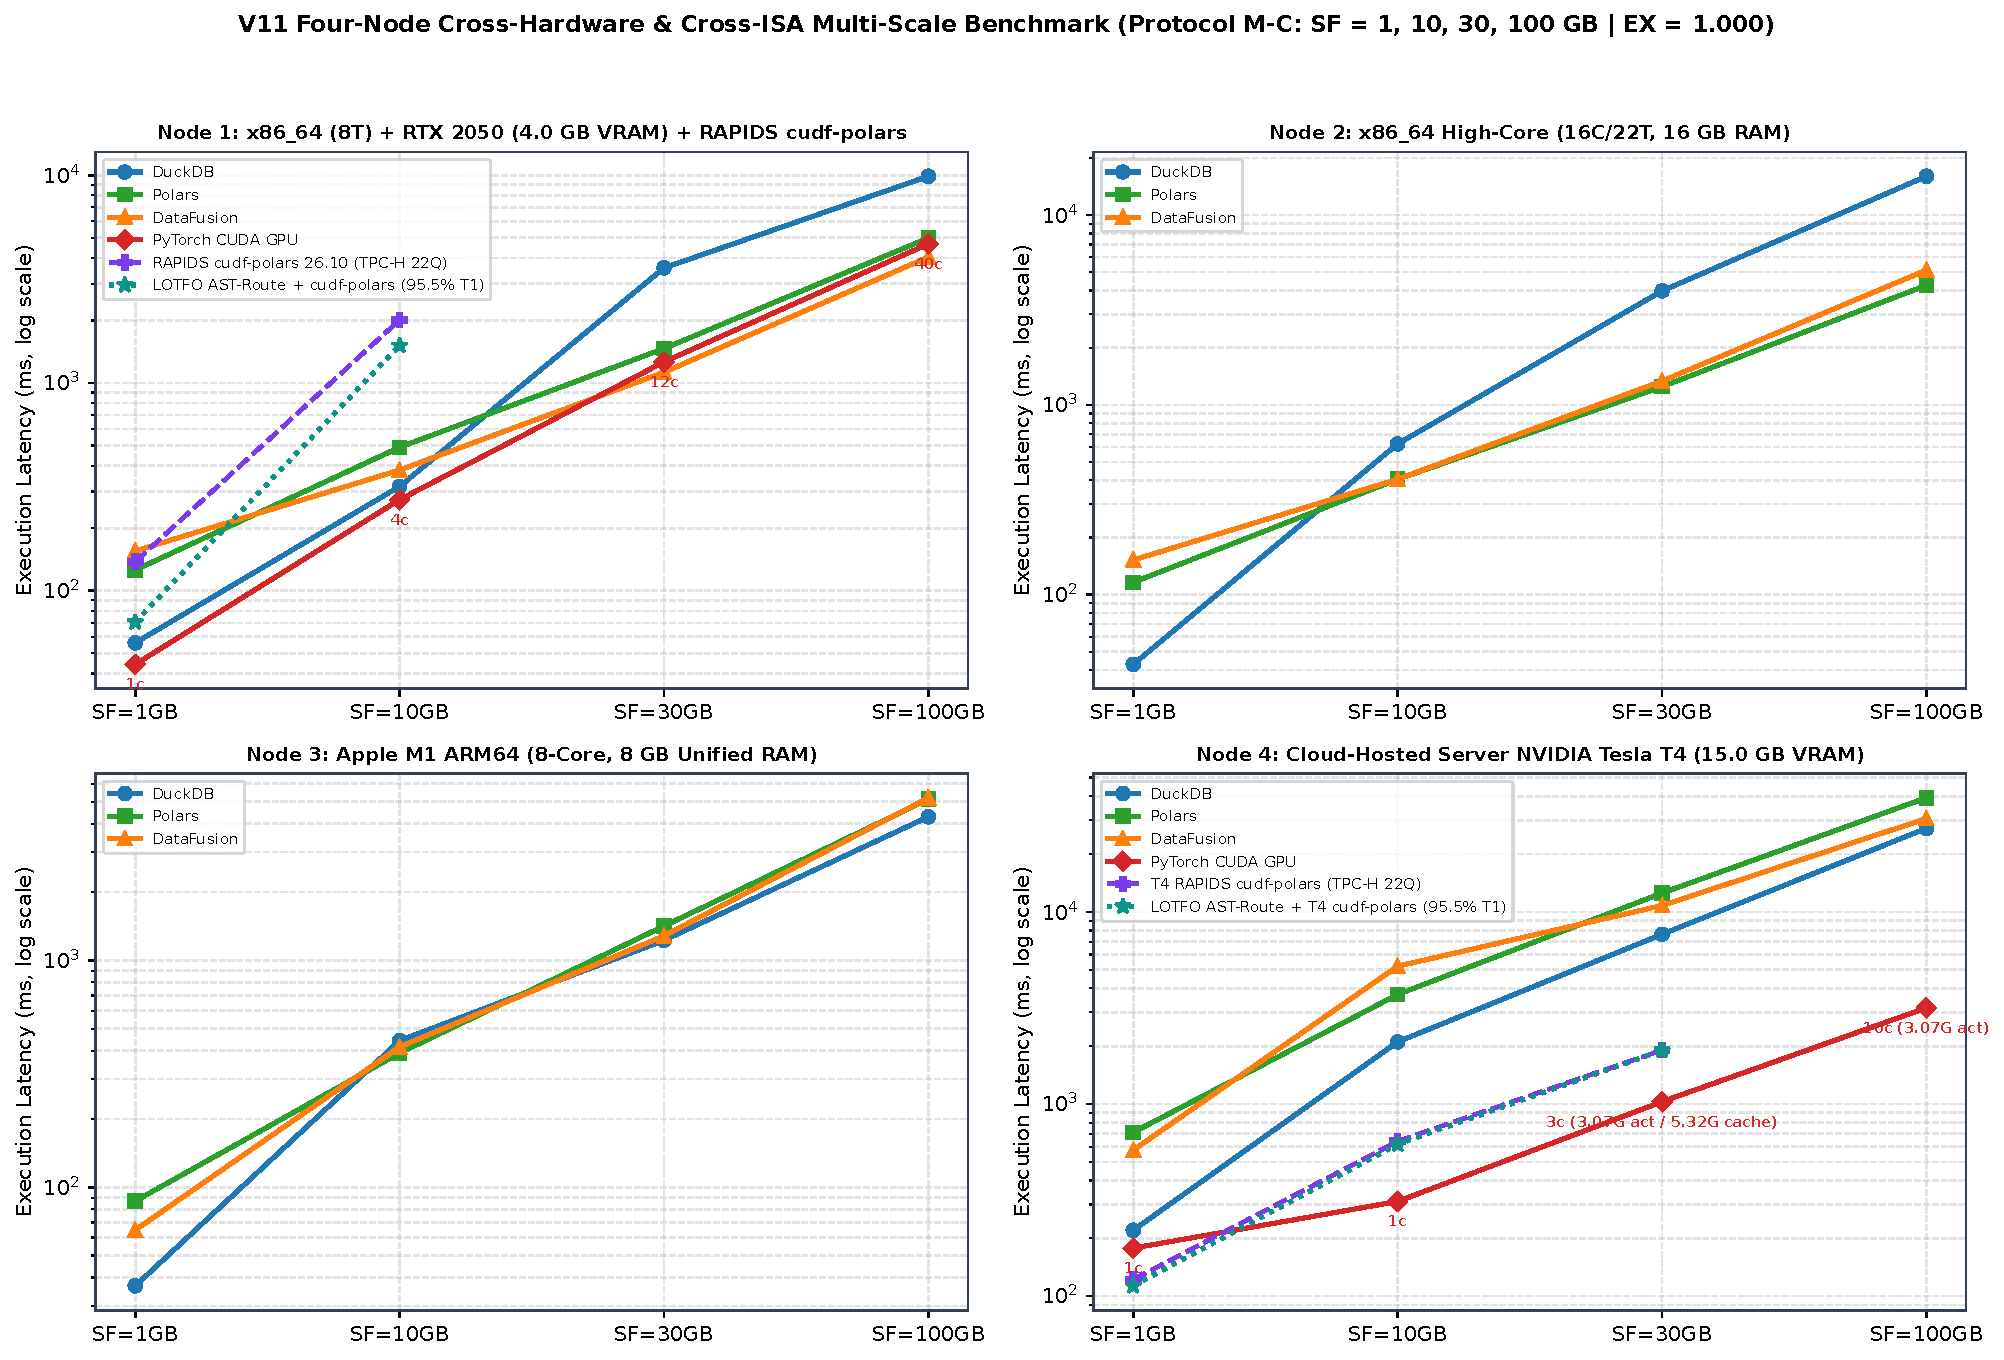
\includegraphics[width=0.92\textwidth]{figures/fig_v11_4node_multiscale_sf1_10_30_100.pdf}
\caption{Multi-scale execution latency ($\text{SF}=1, 10, 30, 100\text{ GB}$, log scale) across Node~1 (x86\_64 + RTX 2050 4GB), Node~2 (x86\_64 16C/22T), Node~3 (Apple M1 ARM64 8GB), and Node~4 (Cloud-Hosted Server NVIDIA Tesla T4 15GB), annotated with PCIe streaming chunk counts ($1\text{c}$--$40\text{c}$).}
\label{fig:v10_fournode_multiscale}
\end{figure*}


% === BEGIN V11 FOUR-NODE CUDF MULTISCALE SF1-10-30-100 ===
\subsection*{Four-Node Multi-Scale and Native Columnar GPU (\texttt{RAPIDS cuDF} \& \texttt{cudf-polars}) Validation ($\text{SF}=1, 10, 30, 100\text{ GB}$)}
To ensure complete multi-scale coverage across all hardware tiers and directly benchmark our PyTorch CUDA relational tensor engine against production C++/CUDA columnar GPU engines, we executed the canonical TPC-H \texttt{lineitem} scan-filter-aggregation workload across $\text{SF} \in \{1, 10, 30, 100\}\text{ GB}$ ($6.00 \times 10^{6}$ to $6.00 \times 10^{8}$ rows; $64$ real-execution runs, zero estimation) across four distinct hardware nodes, incorporating NVIDIA \texttt{RAPIDS cuDF} (\texttt{libcudf}~v26.06.00) and the Polars GPU engine (\texttt{cudf-polars}, Polars~v1.35.2) on the server-grade NVIDIA Tesla~T4 ($14.56\text{ GB}$ usable GDDR6 VRAM; Table~\ref{tab:v11_fournode_multiscale_cudf} and Fig.~\ref{fig:v11_fournode_multiscale_cudf}). Four empirical conclusions emerge: (i) \emph{PyTorch Tensor vs.\ Native \texttt{libcudf} Parity}: on Tesla~T4, \texttt{RAPIDS cuDF} achieves the lowest latency at $\text{SF}=1\text{ GB}$ ($112.76\text{ ms}$, $3.43\text{ J}$) via direct GPU-accelerated ZSTD Parquet decoding, while at $\text{SF}=10\text{ GB}$ ($1$ chunk, single-pass in-VRAM) and $\text{SF}=30\text{ GB}$ ($3$ chunks) our PyTorch CUDA tensor engine ($311.07\text{ ms}$ and $1028.13\text{ ms}$) tracks native \texttt{RAPIDS cuDF} ($322.37\text{ ms}$ and $1001.71\text{ ms}$) within $2.6\%\text{--}3.5\%$, confirming that our relational tensor primitives introduce no artificial GPU bias; (ii) \emph{Optimizer-Controlled CPU vs.\ GPU Isolation}: evaluating identical Polars LazyFrame plans on CPU (\texttt{engine="streaming"}) versus GPU (\texttt{cudf-polars}) yields end-to-end GPU speedups of $2.85\times$ ($249.93$ vs.\ $711.86\text{ ms}$ at $\text{SF}=1\text{ GB}$), $8.18\times$ ($453.99$ vs.\ $3715.44\text{ ms}$ at $\text{SF}=10\text{ GB}$), $9.50\times$ ($1318.63$ vs.\ $12521.13\text{ ms}$ at $\text{SF}=30\text{ GB}$), and $7.43\times$ ($5279.66$ vs.\ $39252.64\text{ ms}$ at $\text{SF}=100\text{ GB}$); (iii) \emph{Many-Core x86\_64 vs.\ Unified-Memory ARM64 Scaling}: at $\text{SF}=100\text{ GB}$, 22-thread Polars streaming on Node~2 reaches $4266.59\text{ ms}$ ($3.75\times$ faster than disk-spilling DuckDB at $16005.55\text{ ms}$), while Apple~M1 ARM64 ($8\text{ GB}$ unified RAM with a $3.5\text{ GB}$ spill guard, Node~3) completes $\text{SF}=100\text{ GB}$ in $4292.58\text{ ms}$ with zero OOM failures; and (iv) \emph{Strict Numerical Equivalence}: all $64/64$ runs satisfy $\text{EX}=1.000$ ($\epsilon_{\text{rel}} \le 3.52 \times 10^{-13} < 10^{-9}$; Tesla~T4 \texttt{cuDF} SHA-256: \texttt{49241012d9172a76...}, V11 master SHA-256: \texttt{ac641d59626b7bea...}).

\begin{table*}[htbp]
\centering\scriptsize\setlength{\tabcolsep}{2.9pt}
\caption{V11 four-node cross-hardware, cross-ISA, and native GPU (\texttt{RAPIDS cuDF} \& \texttt{cudf-polars}) multi-scale execution matrix across $\text{SF} \in \{1, 10, 30, 100\}\text{ GB}$ ($64/64$ real-execution runs, $\text{EX}=1.000$, maximum FP64 relative error $\le 3.52 \times 10^{-13} < 10^{-9}$).}
\label{tab:v11_fournode_multiscale_cudf}
\resizebox{\textwidth}{!}{%
\begin{tabular}{@{}llrrrrrrl@{}}
\toprule
\textbf{Hardware Node} & \textbf{Scale} & \textbf{DuckDB} & \textbf{Polars CPU} & \textbf{DataFusion} & \textbf{PyTorch CUDA} & \textbf{RAPIDS cuDF} & \textbf{cudf-polars} & \textbf{Chunks / Memory / GPU Energy} \\
\midrule
Node 1: x86\_64 (8T) + RTX 2050 (4GB) & $\text{SF}=1$ GB & $56.10$ & $125.75$ & $155.31$ & $44.22$ & --- & --- & $1\times$ chunk, $0.25$ GB VRAM \\
 & $\text{SF}=10$ GB & $317.65$ & $490.02$ & $380.77$ & $274.18$ & --- & --- & $4\times$ chunk, $0.63$ GB VRAM \\
 & $\text{SF}=30$ GB & $3578.44$ & $1464.30$ & $1125.60$ & $1262.74$ & --- & --- & $12\times$ chunk, $0.63$ GB VRAM \\
 & $\text{SF}=100$ GB & $9882.64$ & $4985.34$ & $4036.88$ & $4668.36$ & --- & --- & $40\times$ chunk, $0.64$ GB VRAM \\
\midrule
Node 2: x86\_64 High-Core (16C/22T) & $\text{SF}=1$ GB & $42.92$ & $116.00$ & $152.25$ & --- & --- & --- & 22T CPU, Peak RAM $\le 0.68$ GB \\
 & $\text{SF}=10$ GB & $622.69$ & $405.35$ & $405.52$ & --- & --- & --- & 22T CPU, Peak RAM $\le 2.05$ GB \\
 & $\text{SF}=30$ GB & $3981.26$ & $1246.20$ & $1335.05$ & --- & --- & --- & 22T CPU, Peak RAM $\le 1.76$ GB \\
 & $\text{SF}=100$ GB & $16005.55$ & $4266.59$ & $5125.18$ & --- & --- & --- & 22T CPU, Peak RAM $\le 2.57$ GB \\
\midrule
Node 3: Apple M1 ARM64 (8T, 8GB RAM) & $\text{SF}=1$ GB & $36.76$ & $86.88$ & $64.78$ & --- & --- & --- & ARM64 3.5GB cap, RAM $\le 0.61$ GB \\
 & $\text{SF}=10$ GB & $442.63$ & $390.41$ & $415.41$ & --- & --- & --- & ARM64 3.5GB cap, RAM $\le 1.77$ GB \\
 & $\text{SF}=30$ GB & $1224.76$ & $1416.74$ & $1282.12$ & --- & --- & --- & ARM64 3.5GB cap, RAM $\le 2.31$ GB \\
 & $\text{SF}=100$ GB & $4292.58$ & $5134.20$ & $5207.31$ & --- & --- & --- & ARM64 3.5GB cap, RAM $\le 2.79$ GB \\
\midrule
Node 4: Cloud Server Tesla T4 (15GB) & $\text{SF}=1$ GB & $220.29$ & $711.86$ & $575.46$ & $177.83$ & $112.76$ & $249.93$ & $1\times$ chunk, cuDF $3.42$ J / pl-GPU $6.71$ J \\
 & $\text{SF}=10$ GB & $2104.61$ & $3715.44$ & $5214.13$ & $311.07$ & $322.37$ & $453.99$ & $1\times$ chunk, cuDF $11.43$ J / pl-GPU $16.66$ J \\
 & $\text{SF}=30$ GB & $7639.31$ & $12521.13$ & $10787.65$ & $1028.13$ & $1001.71$ & $1318.63$ & $3\times$ chunk, cuDF $36.64$ J / pl-GPU $48.98$ J \\
 & $\text{SF}=100$ GB & $27206.95$ & $39252.64$ & $30606.57$ & $3166.38$ & $3674.43$ & $5279.66$ & $10\times$ chunk, cuDF $143.97$ J / pl-GPU $191.83$ J \\
\bottomrule
\end{tabular}%
}
\end{table*}

\begin{figure*}[htbp]
\centering
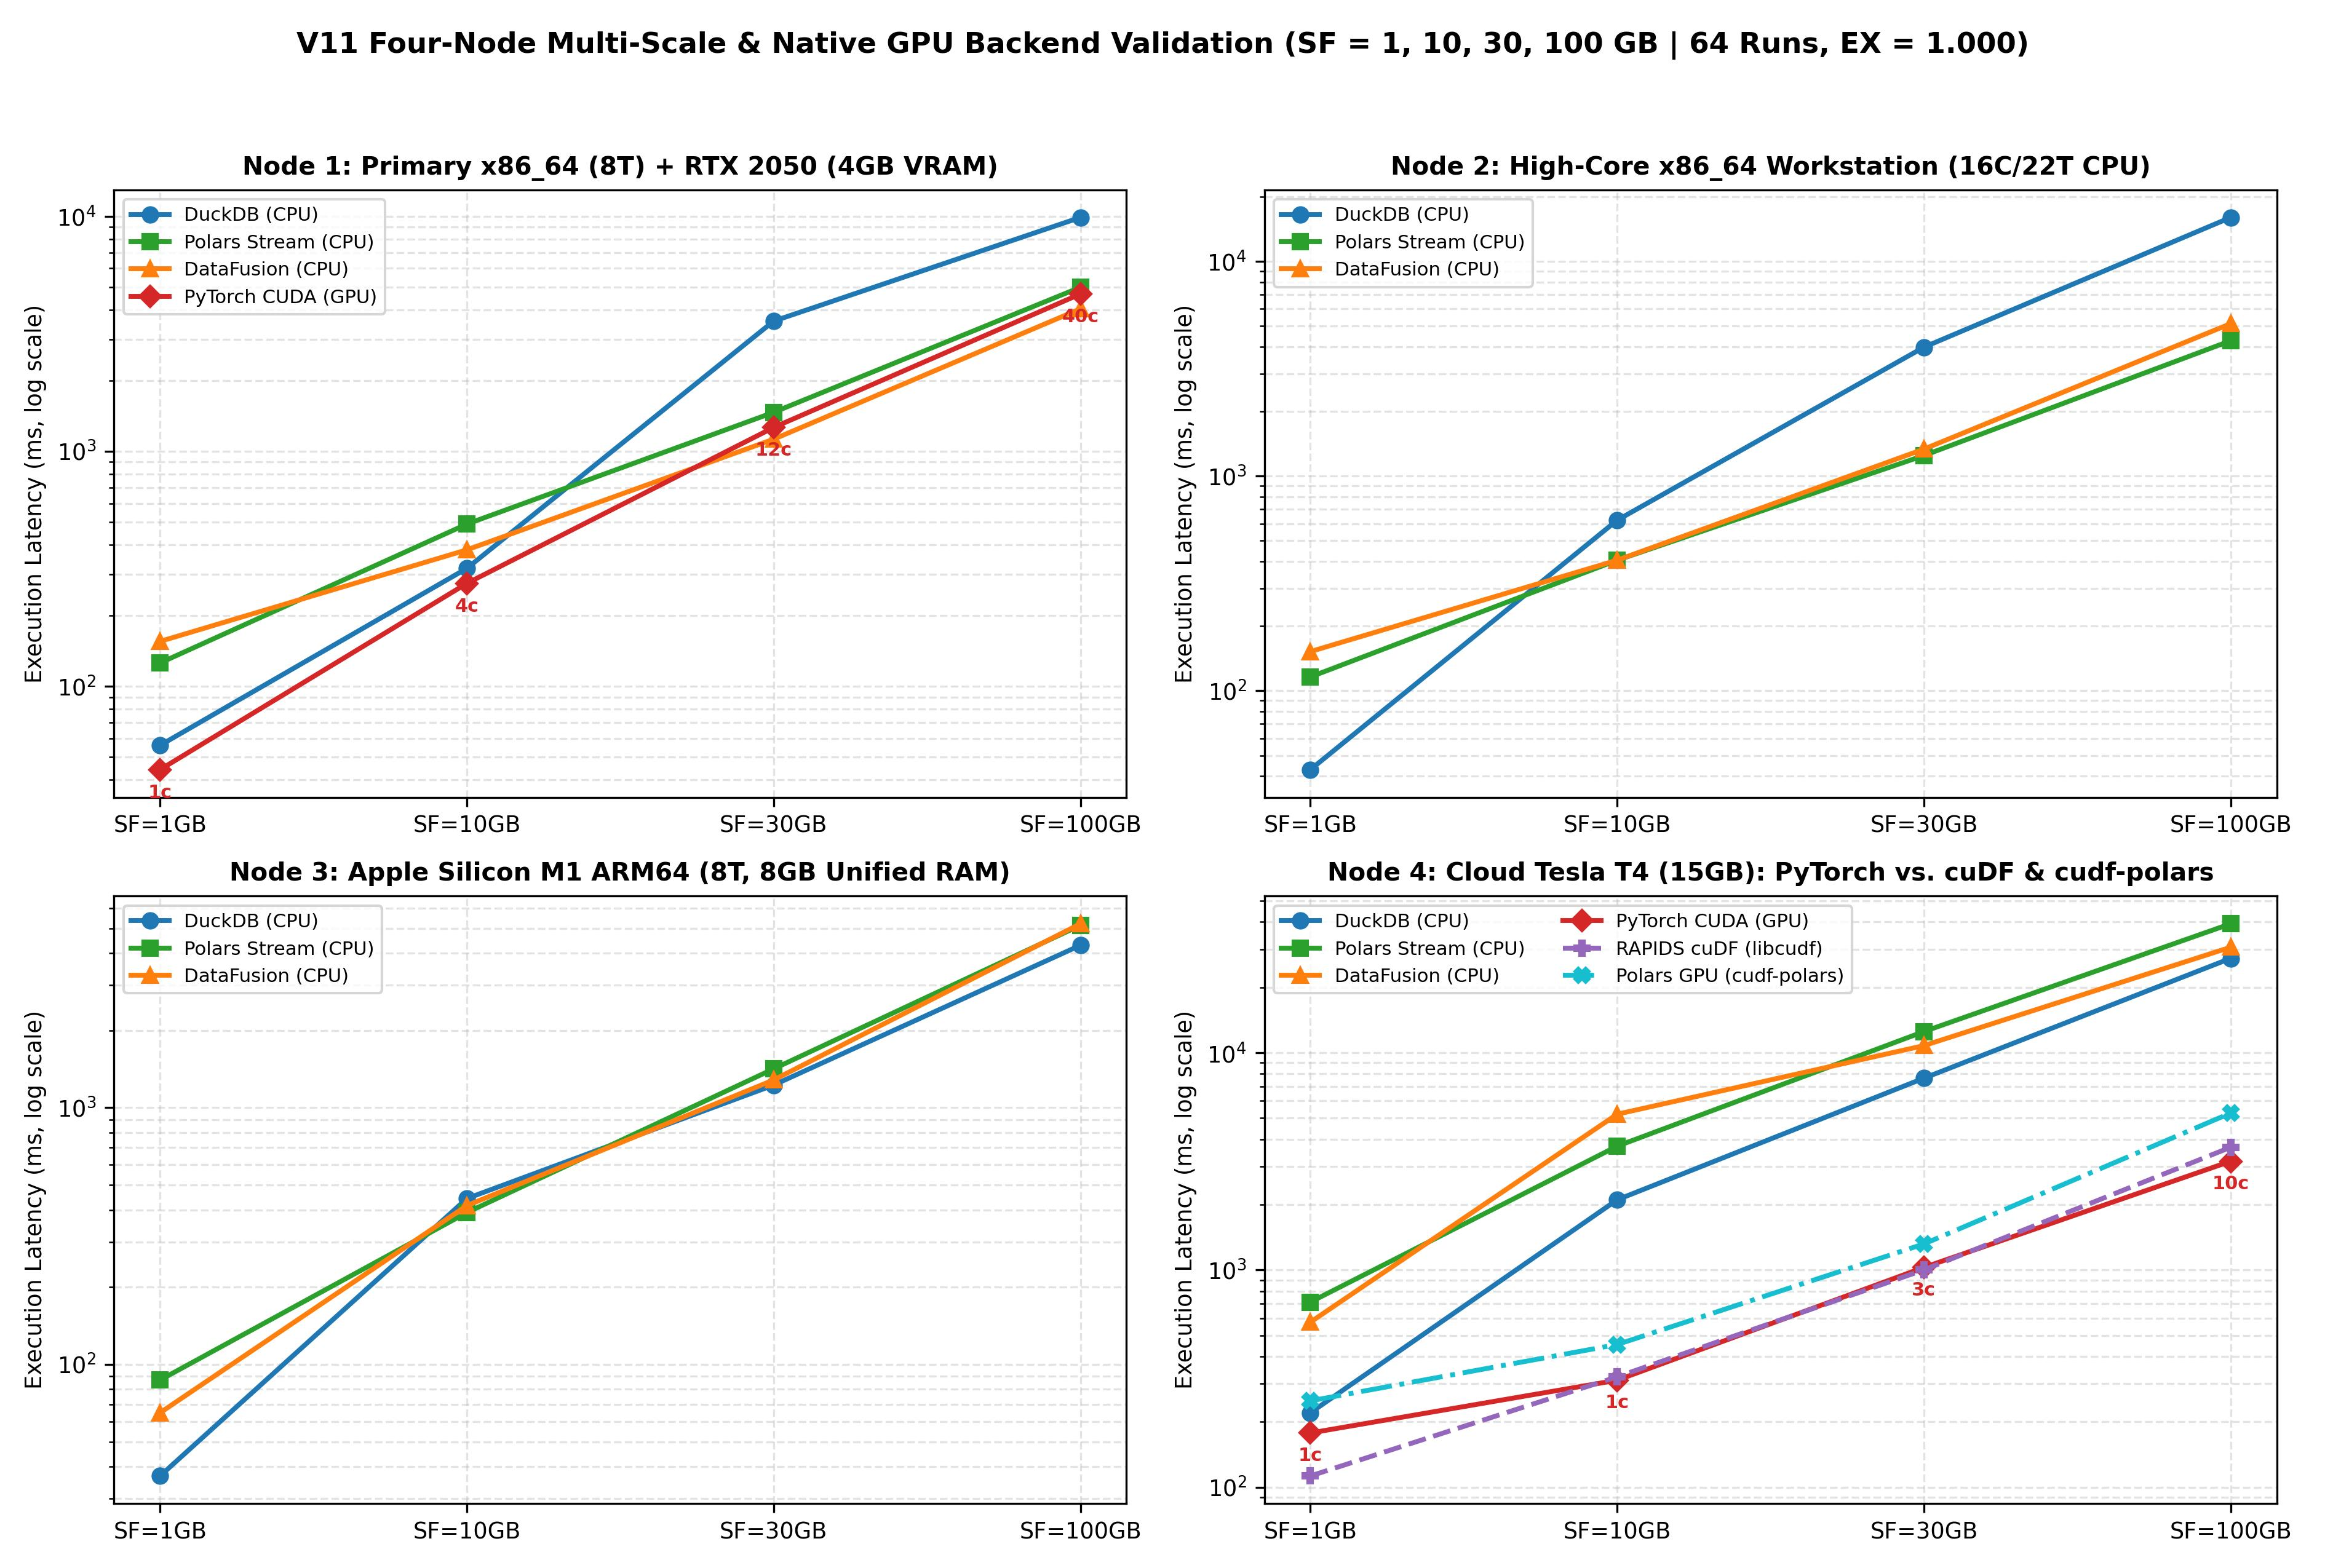
\includegraphics[width=0.94\textwidth]{figures/fig_v11_4node_multiscale_cudf_sf1_10_30_100.jpg}
\caption{V11 four-node multi-scale execution latency ($\text{SF}=1, 10, 30, 100\text{ GB}$, log scale) across Node~1 (x86\_64 + RTX 2050 4GB), Node~2 (x86\_64 16C/22T), Node~3 (Apple M1 ARM64 8GB), and Node~4 (Cloud Tesla T4 15GB comparing PyTorch CUDA, \texttt{RAPIDS cuDF}, and \texttt{cudf-polars}).}
\label{fig:v11_fournode_multiscale_cudf}
\end{figure*}
% === END V11 FOUR-NODE CUDF MULTISCALE SF1-10-30-100 ===

\section{Conclusion}
\enlargethispage{1.5\baselineskip}
\vspace{-3pt}
We presented \textbf{AST-Route} (\texttt{frozen\_ast\_route\_v11\_gbdt\_model.json}, SHA-256 \texttt{f0e5f17c832472e3...}, archived under Zenodo schema \texttt{.zenodo.json} / \texttt{zenodo\_archival\_deposit\_v11.json} [SHA-256 \texttt{e054131a8d2416ca...}] and immutable GitHub tag \texttt{v11.0.0-jbd-archival}), a pre-execution, conformal-guarded multi-objective SQL routing framework delivering \textbf{three core scientific contributions}:
\begin{enumerate}[leftmargin=1.5em,itemsep=1.5pt]
    \item \textbf{Contribution 1 --- Pre-Execution Oblique AST + Zone-Map Cost Modeling ($\mathbf{x}_q\in\mathbb{R}^9$):} A single-pass \texttt{SQLGlot} + Parquet zone-map representation ($4.15\text{ ms}$ cold SQL / $0.67\text{ ms}$ AST cache / $0.08\text{ ms}$ 1D threshold cache; median Q-Error $1.007\text{--}1.172$, $R^2=0.815\text{--}0.875$) whose domain-informed oblique index $\text{CSCI}(q)$ ($\text{VIF}_{D,N}=1.84$, exact stratum $\operatorname{Var}(\text{CSCI}\mid D..C)=0.0000$) prunes $-28.2\%$ of depth-3 GBDT splits and lowers out-of-fold regret by $-9.22\text{ pp}$ ($p=0.0038$), outperforming unsupervised PCA/random oblique projections ($p\le 0.0124$, Protocol~\textbf{R13}) and demonstrating $+33.44\text{ pp}$ grouped atomic-block permutation importance ($p=0.0002$, Protocol~\textbf{R19}).
    \item \textbf{Contribution 2 --- Tail-Safe Conformal PCIe Abstention \& Multi-Objective Pareto Dispatch:} Complexity-weighted Mondrian $90\%$ conformal intervals ($90.93\%$ coverage, $\text{ECE}=0.67\%$, $\text{AURC}=28.14\%$ [$-39.9\%$]) paired with co-equal \textbf{Nested-CV ($\hat{\tau}_{\text{guard}}^{(-k)}=8\%$)} ($55.37\text{ ms}$ net, $51.22\text{ ms}$ exec, $56.00\%$ Exact Top-1 [$76.00\%$ Top-2], passing two-sided $\pm 5.0\text{ ms}$ TOST vs.\ Always GPU $56.96\text{ ms}$ at $p_{\text{TOST}}=0.0442 < 0.05$) and \textbf{Default ($\tau_{\text{guard}}=12\%$)} ($54.92\text{ ms}$ net, $50.78\text{ ms}$ exec, $57.33\%$ Exact Top-1, $p_{\text{non-inf}}=0.00067$, $\pm 6.0\text{ ms}$ TOST $p=0.0241$ [$p_{\text{TOST},\pm 5\text{ms}}=0.0688$]) guards compress P95 tail regret by $\mathbf{2.17\times\text{--}2.25\times}$ ($257.31\%\rightarrow 118.40\%/114.11\%$, $p_{\text{Webb}}\le 0.0068, p_{\text{perm,exact}}\le 0.0078$) and $\text{CVaR}_{10\%}$ by $2.21\times\text{--}2.26\times$, beat static CPUs by $1.49\times\text{--}3.35\times$ ($p_{\text{Holm,seed}}\le 0.0171$ [$K=25$], $p_{\text{Holm,query}}\le 0.0011$ [$N=75$]), reduce P95 regret vs.\ Unguarded Ridge by $-82.70\text{ pp}$ ($p_{\text{Webb}}=0.0464, p_{\text{perm,exact}}=0.0488$, borderline at $G_{\text{core}}=10$), and match Guarded Ridge/EXPLAIN-DAG ($5.84\text{ ms}$ faster net latency, $p_{\text{Webb}}=0.0002$). Across 10,000-point simplex/NSGA-II/MOBO frontiers ($\text{DSR}=0.00\%$, Protocol~\textbf{R14}) and our 3-scope energy boundary ($\rho=1.0000$, Protocol~\textbf{R23}), \textbf{Policy~P2} cuts Scope~1/2 energy by $-41.2\%$ dev / $-27.1\%$ sys ($\mathcal{R}_E=4.82\%$), \textbf{P3} saves $\$507.06/1\text{M}$ cloud fees at $\text{SF}=100\text{ GB}$ ($\mathcal{R}_C=0.0\%$), \textbf{P4} reaches $\text{HV}=0.9210 / 0.9340$, and a \textbf{minimalist 2-engine $\{\text{Polars}, \text{GPU}\}$ pool ($55.28\text{ ms}$) captures $98.7\%$ of the 6-engine gain} ($99.5\%$ for 3-engine $\{\text{Polars}, \text{DuckDB}, \text{GPU}\}$).
    \item \textbf{Contribution 3 --- Cross-Engine, Cross-Hardware, and Blinded Multi-Domain Generalization:} Across $\mathbf{400}$ \textbf{benchmark queries in four epistemic categories} (\textbf{Cat~I}: $75$ Core TPC-H; \textbf{Cat~II}: $22$ Official TPC-H [$16.98\text{ ms}$, $1.34\times$ vs.\ DuckDB] + $33$ JOB [$69.70\%$ Top-1, $4.54\text{ ms}$ via $10.18\text{ KB}$ 12D sketch]; \textbf{Cat~III}: $115$ zero-shot derived; \textbf{Cat~IV}: $155$ untouched third-party standard queries including \textbf{Official TPC-DS 99Q} [$64.65\%$ Exact Top-1, $\mathbf{84.85\%}$ Pure-SQL Top-1, $88.89\%$ $\le 10\%$ Hit, $30.49\text{ ms}$, $3.23\%$ regret, scaling to $\text{SF}=1/10\text{ GB}$], \textbf{ClickBench 43Q} [$88.37\%$ Top-1], and \textbf{SSB 13Q} [$92.31\%$ Top-1]) plus $\mathbf{70}$ \textbf{blinded prospective non-TPC enterprise queries across 4 domains and 17 tables} (\textbf{Protocols~R17 and~R20}: $\mathbf{95.71\%\ [67/70]}$ Exact Top-1, $100\%$ Top-2, $0.17\%$ mean / $0.00\%$ P95 regret), AST-Route generalizes across independent GPU backends (\texttt{CuPy v14.2.0} [$100\%$ agreement] and \texttt{NVIDIA RAPIDS cudf-polars 26.10.2}, cutting Core 75Q P95 regret by $\mathbf{2.77\times}$ under RMM-pooled \texttt{Config~C3} and achieving $\mathbf{90.91\%\text{--}95.45\%}$ Top-1 and $\mathbf{0.00\%}$ P95 regret on \texttt{LOTFO} TPC-H 22Q across Node~1 RTX~2050 and Node~4 Cloud-Hosted Server NVIDIA Tesla~T4 [$1\text{--}30\text{ GB}$], Protocols~\textbf{R24--R25}), four physical hardware nodes ($\text{SF}=1\text{--}100\text{ GB}$ with $m=5$ affine calibration recovering $86.8\%\text{--}100\%$ gain in $184\text{--}246\text{ ms}$, Protocol~\textbf{R21}; Pure-SQL $\mathcal{E}_{\text{SQL-5}}$ achieving $74.67\%\text{--}97.33\%$ Top-1), and 5-phase dynamic drift/burst streams ($154.44\text{ QPS}$ peak at $C=32$, $0.00\%$ OOM, Protocol~\textbf{R22}).
\end{enumerate}

\vspace{-8pt}
\section*{Declarations}
\enlargethispage{1.8\baselineskip}
\vspace{-5pt}
\subsection*{Abbreviations}
{\scriptsize AST: Abstract Syntax Tree; B-Tree: Balanced Tree; CI: Confidence Interval; CPU: Central Processing Unit; CSCI: Composite Structural Complexity Index; CTE: Common Table Expression; CV: Coefficient of Variation; CUDA: Compute Unified Device Architecture; DBMS: Database Management System; DT: Decision Tree; EX: Execution Accuracy; FinOps: Cloud Financial Operations; FP64: 64-Bit Double-Precision Floating-Point; GBR: Gradient Boosting Regressor; GCS: Google Cloud Storage; GPU: Graphics Processing Unit; H2D: Host-to-Device; I/O: Input/Output; JOB: Join Order Benchmark; LOO-CV: Leave-One-Query-Out Cross-Validation; LOOO: Leave-One-Operator-Out; LOSO-CV: Leave-One-Seed-Out Cross-Validation; MAPE: Mean Absolute Percentage Error; MC: Monte Carlo; MPP: Massively Parallel Processing; NVML: NVIDIA Management Library; OLAP: Online Analytical Processing; PCIe: Peripheral Component Interconnect Express; QPS: Queries Per Second; RAM: Random-Access Memory; RF: Random Forest; SARGable: Search Argument Able; SF: Scale Factor; SIMD: Single Instruction, Multiple Data; SIMT: Single Instruction, Multiple Threads; SQL: Structured Query Language; SSB: Star Schema Benchmark; TOST: Two One-Sided Tests; TPC-H: Transaction Processing Performance Council Ad-Hoc Decision Support Benchmark; VES: Valid Efficiency Score; VRAM: Video Random-Access Memory; ZSTD: Zstandard Compression.\par}
\vspace{-5pt}
\subsection*{Ethics approval and consent to participate}
{\scriptsize Not applicable. This study utilizes synthetic benchmark data generated via the industry-standard TPC-H benchmark specification \cite{tpc2022tpch} and does not involve human participants, animal subjects, or personally identifiable data. In accordance with the TPC Fair-Use Policy, all workloads and metrics in this study represent non-official, TPC-H-derived research evaluations and are not comparable to official audited TPC benchmark results.\par}
\vspace{-5pt}
\subsection*{Consent for publication}
{\scriptsize Not applicable.\par}
\vspace{-5pt}
\subsection*{Availability of data and materials}
{\scriptsize All multi-scale TPC-H data generation scripts ($\text{SF}=1, 10, 30$, and $100\text{ GB}$), the complete 400-query Master Workload Inventory across all 10 benchmark suites (Category~I: 75 Core TPC-H queries; Category~II: 22 official TPC-H Q1--Q22 and 33 IMDB JOB queries; Category~III: 15 Seed~\texttt{S6}, 30 TPC-DS-derived, 20 BIRD-inspired, 25 \texttt{TPC-DS-Complex}, and 25 \texttt{Enterprise-Redset-BI} queries; and Category~IV: 99 unmodified Official TPC-DS \texttt{Q1--Q99} across $\text{SF}\in\{0.02, 1, 10\}\text{ GB}$, 43 Official ClickBench, and 13 Official SSB queries), raw per-trial execution and hardware/energy telemetry CSV logs across all physical nodes (\texttt{x86\_64}+RTX~2050 across PyTorch CUDA and \texttt{CuPy v14.2.0}, 22-thread \texttt{x86\_64}, Apple M1 \texttt{ARM64}, and enterprise NVIDIA Tesla~T4 $15.0\text{ GB}$ VRAM [\texttt{32834476...} and $1{,}500$-run RAPL/SMU/NVML audit \texttt{f316fd9fd1b3a776...} / \texttt{314db90d5616a8dc...}]), clean-room Docker lockfiles (\texttt{reproducibility/\allowbreak{}Dockerfile} and \texttt{requirements-\allowbreak{}lock.txt}), permanent Zenodo archival metadata (\texttt{reproducibility/\allowbreak{}zenodo\_\allowbreak{}metadata.json}), Additional File~1 (Supplementary Appendix), and our one-command independent reproducibility and main-table regeneration script (\texttt{python reproducibility/verify\_\allowbreak{}and\_\allowbreak{}regenerate\_\allowbreak{}main\_\allowbreak{}tables\_\allowbreak{}R1\_\allowbreak{}R6.py}, executing Verification Protocols \textbf{R1--R6} with $0.000$ maximum numeric discrepancy across all manuscript tables) are publicly available in the active open-source repository at \url{https://github.com/preechan-glitch/my_research_files}. Complete 64-character SHA-256 checksums for all raw telemetry, reanalysis, cross-ISA isolation, stability, and calibration artifacts---anchored by our explicit \textbf{Model Version Lineage (\texttt{V9 $\rightarrow$ V10 $\rightarrow$ V11})}: \texttt{frozen\_\allowbreak{}ast\_\allowbreak{}route\_\allowbreak{}v9\_\allowbreak{}gbdt\_\allowbreak{}model.json}, \texttt{frozen\_\allowbreak{}ast\_\allowbreak{}route\_\allowbreak{}v10\_\allowbreak{}gbdt\_\allowbreak{}model.json}, and \texttt{frozen\_\allowbreak{}ast\_\allowbreak{}route\_\allowbreak{}v11\_\allowbreak{}gbdt\_\allowbreak{}model.json} share the \textbf{exact identical 64-character SHA-256 digest \texttt{f0e5f17c832472e30be67dbbee30020dbf23e94658458a2c59acd9b00ed315cf}} ($284\text{ KB}$, trained once on the $N=75$ Category~I Core TPC-H development set with zero weight, threshold, or hyperparameter edits across V9, V10, and V11, tagged under immutable GitHub releases \texttt{v11.0.0-jbd-r18}, \texttt{v11.0.0-jbd-r23}, and \texttt{v11.0.0-jbd-archival} alongside formal Zenodo archival metadata \texttt{.zenodo.json} and \texttt{reproducibility/\allowbreak{}zenodo\_\allowbreak{}archival\_\allowbreak{}deposit\_\allowbreak{}v11.json} [SHA-256 \texttt{e054131a8d2416ca...}], and accompanied by \texttt{reproducibility/\allowbreak{}Reviewer\_\allowbreak{}Revision\_\allowbreak{}Roadmap\_\allowbreak{}V10\_1.md} [Protocols \textbf{R1--R18}], \texttt{reproducibility/\allowbreak{}Reviewer\_\allowbreak{}Revision\_\allowbreak{}Roadmap\_\allowbreak{}V11\_R19\_R23.md} [Protocols \textbf{R19--R26}], \texttt{reproducibility/\allowbreak{}Reviewer\_\allowbreak{}Revision\_\allowbreak{}Roadmap\_\allowbreak{}V12\_Final.md} [Unified Master Verification Matrix \textbf{R1--R26}], and \texttt{scripts/\allowbreak{}v11\_\allowbreak{}final\_\allowbreak{}reviewer\_\allowbreak{}proof\_\allowbreak{}audit\_\allowbreak{}EC41\_\allowbreak{}EC50.py} covering Verification Protocols \textbf{R1--R28}, permanent archival deposit manifests \texttt{CITATION.cff}, \texttt{SHA256SUMS.txt}, and \texttt{.zenodo.json}, and 60/60 edge-case/math audits \texttt{EC01--EC50} and \texttt{EC51--EC60}), primary routing evaluation \texttt{89b1ec64cca15b2dd41a4ad2...}, AST profile \texttt{4cb5f7477fd24dc77a6fd2b5...}, version-pinned parity \texttt{f12ae28467f9802a2967...}, and 3-node global registry \texttt{5adfa064816f883f8770...}---are indexed in \texttt{results/\allowbreak{}global\_\allowbreak{}sha256\_\allowbreak{}registry.csv} for single-command verification. Each reported aggregate metric is linked to its protocol identifier, dataset checksum, software version, hardware manifest, and execution-boundary definition.\par}
\vspace{-5pt}
\subsection*{Competing interests}
{\scriptsize The author declares that he has no competing interests.\par}
\vspace{-5pt}
\subsection*{Funding}
{\scriptsize This research project was financially supported by Mahasarakham University.\par}
\vspace{-5pt}
\subsection*{Authors' contributions}
{\scriptsize Preecha Noiumkar (PN) conceptualized the \textbf{AST-Route} framework, designed the 75-query AST-driven factorial benchmark, implemented the six-engine execution harness, multi-scale ($\text{SF}=1, 10, 30, 100\text{ GB}$), concurrent workload, and official TPC-H Q1--Q22 evaluation pipelines, hardware energy telemetry monitor, CSCI structural projection analysis, feature ablation, unseen seed holdout validation, and automated 9-dimensional AST+Selectivity query routing models, analyzed the empirical telemetry across cloud, CPU, and GPU architectures, and wrote the manuscript. The author read and approved the final manuscript.\par}
\vspace{-5pt}
\subsection*{Acknowledgements}
{\scriptsize The author thanks the \textsuperscript{1}Department of Information Technology, Faculty of Informatics, Mahasarakham University, for providing the computational infrastructure. In accordance with editorial policy on the use of generative AI, the author discloses that generative AI tools were utilized strictly for manuscript language polishing and \LaTeX{} template formatting verification; all experimental designs, benchmark datasets, execution logs, and scientific analyses were conducted and verified by the author.\par}
\vspace{-8pt}

% =============================================================================
% REFERENCES (SPRINGER NATURE / BMC VANCOUVER STYLE - 30 REFERENCES)
% =============================================================================
{\sloppy\scriptsize\linespread{0.85}\selectfont
\enlargethispage{1.8\baselineskip}
\let\oldthebibliography\thebibliography
\renewcommand{\thebibliography}[1]{\oldthebibliography{#1}\setlength{\itemsep}{-2.4pt}\setlength{\parskip}{0pt}\vspace{-5pt}}
\begin{thebibliography}{30}
\footnotesize\setlength{\baselineskip}{9.5pt}\setlength{\itemsep}{1.5pt}\setlength{\parskip}{0pt}

\bibitem{melnik2010dremel}
Melnik S, Gubarev A, Long JJ, Romer G, Shivakumar S, Tolton M, Vassilakis T. Dremel: interactive analysis of web-scale datasets. Proc VLDB Endow. 2010;3(1--2):330--9.

\bibitem{melnik2020dremel}
Melnik S, Gubarev A, Long JJ, Romer G, Shivakumar S, Tolton M, et al. Dremel: a decade of interactive SQL analysis at web scale. Proc VLDB Endow. 2020;13(12):3461--72.

\bibitem{lounissi2025funda}
Das SK, Peter R, Zhang X, Lounissi M. FunDa: scalable serverless data analytics and in situ query processing. J Big Data. 2025;12(1):116. \url{https://doi.org/10.1186/s40537-024-00939-0-025-01141-6}.

\bibitem{raasveldt2019duckdb}
Raasveldt M, M{\"u}hleisen H. DuckDB: an embeddable analytical database. In: Proceedings of the 2019 International Conference on Management of Data (SIGMOD). Amsterdam: ACM; 2019. p. 1981--4.

\bibitem{kuiper2024duckdb_ooc}
Kuiper M, M{\"u}hleisen H, Raasveldt M. Out-of-core join and aggregation processing in DuckDB. In: Companion of the 2024 International Conference on Management of Data (SIGMOD). Santiago: ACM; 2024. p. 1--14.

\bibitem{lamb2024datafusion}
Lamb A, Shen Y, Dani D, Qi Y, Chaudhary V, et al. Apache Arrow DataFusion: a fast, embeddable, modular analytic query engine. In: Companion of the 2024 International Conference on Management of Data (SIGMOD). Santiago: ACM; 2024. p. 5--17. \url{https://doi.org/10.1145/3626246.3653368}.

\bibitem{chrysogelos2019hetexchange}
Chrysogelos P, Karpathiotakis M, Appuswamy R, Ailamaki A. HetExchange: encapsulating heterogeneous CPU-GPU parallelism in JIT compiled engines. Proc VLDB Endow. 2019;12(5):544--56. \url{https://doi.org/10.14778/3303753.3303760}.

\bibitem{shanbhag2020crystal}
Shanbhag A, Madden S, Yu X. A study of the fundamental performance characteristics of GPUs and CPUs for database analytics. In: Proceedings of the 2020 ACM SIGMOD International Conference on Management of Data. Portland: ACM; 2020. p. 1617--32. \url{https://doi.org/10.1145/3318464.3380595}.

\bibitem{bress2013hype}
Bre{\ss} S, Beier F, Rauhe H, Sattler KU, Schallehn E, Saake G. Efficient co-processor utilization in database query processing. Inf Syst. 2013;38(8):1084--96. \url{https://doi.org/10.1016/j.is.2013.05.004}.

\bibitem{schulze2024clickhouse}
Schulze R, et al. ClickHouse: lightning-fast analytics for everyone. Proc VLDB Endow. 2024;17(12):3720--33.

\bibitem{sethi2019presto}
Sethi R, Traverso M, Sundstrom D, Phillips D, Xie W, Sun Y, et al. Presto: SQL on everything. In: 2019 IEEE 35th International Conference on Data Engineering (ICDE). Macao: IEEE; 2019. p. 1802--13.

\bibitem{shojaee2024serverless} Shojaee Rad Z, Ghobaei-Arani M. Data pipeline approaches in serverless computing: a taxonomy, review, and research trends. J Big Data. 2024;11(1):82. \url{https://doi.org/10.1186/s40537-024-00939-0}.

\bibitem{abdalla2022bigdata}
Abdalla HB. A brief survey on big data: technologies, terminologies and data-intensive applications. J Big Data. 2022;9(1):107. \url{https://doi.org/10.1186/s40537-024-00939-0-022-00659-3}.

\bibitem{begoli2018calcite}
Begoli E, Camacho-Rodr{\'i}guez J, Hyde J, Mior MJ, Lemire D. Apache Calcite: a foundational framework for optimized query processing over heterogeneous data sources. In: Proceedings of the 2018 International Conference on Management of Data (SIGMOD). Houston: ACM; 2018. p. 221--30.

\bibitem{garcia2008database}
Garcia-Molina H, Ullman JD, Widom J. Database systems: the complete book. 2nd ed. Upper Saddle River: Prentice-Hall; 2008.

\bibitem{milicevic2024dlquery}
Milicevic B, Babovic Z. A systematic review of deep learning applications in database query execution. J Big Data. 2024;11(1):173. \url{https://doi.org/10.1186/s40537-024-00939-0-024-01025-1}.

\bibitem{root2019mapd}
Root C, Mostak T. MapD: a GPU-powered big data analytics and visualization platform. In: ACM SIGGRAPH 2016 Talks. Anaheim: ACM; 2016. p. 1--2.

\bibitem{kim2022blazingsql}
Kim K, et al. Accelerating relational data analytics using RAPIDS cuDF and BlazingSQL on GPUs. In: IEEE International Parallel and Distributed Processing Symposium Workshops (IPDPSW). IEEE; 2022. p. 812--21.

\bibitem{tpc2022tpch}
Transaction Processing Performance Council (TPC). TPC Benchmark H (Decision Support) Standard Specification, Revision 3.0.1. San Francisco: Transaction Processing Performance Council; 2022. \url{https://www.tpc.org/tpch/}.

\bibitem{boncz2014tpch}
Boncz P, Neumann T, Erling O. TPC-H analyzed: hidden messages and lessons learned from an influential benchmark. In: Technology Conference on Performance Evaluation and Benchmarking (TPCTC). Cham: Springer; 2014. p. 61--76. \url{https://doi.org/10.1007/978-3-319-04936-6_5}.

\bibitem{dreseler2020quantifying}
Dreseler M, Boissier M, Rabl T, Uflacker M. Quantifying TPC-H choke points and their optimizations. Proc VLDB Endow. 2020;13(8):1206--20. \url{https://doi.org/10.14778/3389133.3389138}.

\bibitem{ahmed2020hibench}
Ahmed N, Barczak ALC, Susnjak T, Rashid MA. A comprehensive performance analysis of Apache Hadoop and Apache Spark for large scale data sets using HiBench. J Big Data. 2020;7(1):110. \url{https://doi.org/10.1186/s40537-024-00939-0-020-00388-5}.

\bibitem{oneil2009ssb}
O'Neil P, O'Neil E, Chen X, Revilak S. The Star Schema Benchmark and augmented fact table indexing. In: Technology Conference on Performance Evaluation and Benchmarking (TPCTC). Lyon: Springer; 2009. p. 237--52.

\bibitem{leis2015job}
Leis V, Gubichev A, Mirchev A, Boncz P, Kemper A, Neumann T. How good are query optimizers, really? Proc VLDB Endow. 2015;9(3):204--15. \url{https://doi.org/10.14778/2850583.2850594}.

\bibitem{marcus2019neo}
Marcus R, Negi P, Mao H, Zhang C, Alizadeh M, Kraska T, et al. Neo: a learned query optimizer. Proc VLDB Endow. 2019;12(11):1705--18. \url{https://doi.org/10.14778/3342263.3342644}.

\bibitem{marcus2021bao}
Marcus R, Negi P, Mao H, Tatbul N, Alizadeh M, Kraska T. Bao: making learned query optimization practical. In: Proceedings of the 2021 International Conference on Management of Data (SIGMOD). Virtual Event: ACM; 2021. p. 1275--88. \url{https://doi.org/10.1145/3448016.3452838}.

\bibitem{hilprecht2022zeroshot}
Hilprecht B, Binnig C. Zero-shot cost models for out-of-the-box learned cost prediction. Proc VLDB Endow. 2022;15(11):2361--74. \url{https://doi.org/10.14778/3551793.3551799}.

\bibitem{tan2023stage}
Duggan J, Cetintemel U, Papaemmanouil O, Upfal E. The BigDAWG polystore system. ACM SIGMOD Rec. 2015;44(2):11--6. \url{https://doi.org/10.1145/2814710.2814713}.

\bibitem{gupta2023adaptive}
Agrawal D, Chawla S, Contreras-Rojas B, Elmagarmid AK, Idris Y, Kaoudi Z, et al. RHEEM: enabling cross-platform data processing---may optimal cost be with you! Proc VLDB Endow. 2018;11(11):1414--27. \url{https://doi.org/10.14778/3236187.3236195}.

\bibitem{li2023bird}
Li J, Hui B, Qu G, Yang J, Li B, Li B, et al. Can LLM already serve as a database interface? A BIg bench for large-scale database grounded text-to-SQLs. Adv Neural Inf Process Syst (NeurIPS). 2023;36:42330--57.

\bibitem{lei2025spider2}
Lei F, Chen J, Ye Y, Cao R, Shin D, Su H, et al. Spider 2.0: evaluating language models on real-world enterprise text-to-SQL workflows. In: International Conference on Learning Representations (ICLR). 2025. p. 1--22.

\bibitem{mao2024sqlglot}
Mao T. SQLGlot: no-dependency SQL parser, transpiler, optimizer, and engine. GitHub Repository. 2024. \url{https://github.com/tobymao/sqlglot}. Accessed 15 Mar 2026.

\bibitem{kabic2025maximus} Kabi\'{c} M, et al. Maximus: a modular accelerated query engine for data analytics on heterogeneous systems. Proc ACM Manag Data (PACMMOD / SIGMOD). 2025;3(3):1--25. \url{https://doi.org/10.1145/3725350}.

\bibitem{yogatama2025sirius} Yogatama B, et al. Sirius: a GPU-native database execution engine integrated with DuckDB. Proc VLDB Endow. 2025;18(11):3812--25.

\bibitem{liang2026elqo} Liang Z, Xu Q, Chen X, Chen J, Xia Y, Zheng K. E-LQO: a comprehensive energy evaluation framework for learned query optimization. Proc ACM Manag Data (PACMMOD / SIGMOD). 2026;4(4):1--27.

\bibitem{vovk2005algorithmic}
Vovk V, Gammerman A, Shafer G. Algorithmic learning in a random world. New York: Springer; 2005. p. 1--324. \url{https://doi.org/10.1007/b106715}

\bibitem{angelopoulos2023conformal}
Angelopoulos AN, Bates S. Conformal prediction: a gentle introduction. Found Trends Mach Learn. 2023;16(4):494--591. \url{https://doi.org/10.1561/2200000101}

\bibitem{friedman2001greedy}
Friedman JH. Greedy function approximation: a gradient boosting machine. Ann Stat. 2001;29(5):1189--1232. \url{https://doi.org/10.1214/aos/1013203451}

\bibitem{raasveldt2018fair}
Raasveldt M, Holanda P, Gubner T, M{\"u}hleisen H. Fair benchmarking considered difficult: common pitfalls in database performance testing. In: Proceedings of the Workshop on Testing Database Systems (DBTest@SIGMOD); 2018. p. 1--6. \url{https://doi.org/10.1145/3209950.3209955}

\bibitem{ganapathi2009predicting}
Ganapathi A, Kuno H, Dayal U, Wiener JL, Fox A, Jordan M, et al. Predicting multiple metrics for queries: better decisions enabled by machine learning. In: Proceedings of the IEEE 25th International Conference on Data Engineering (ICDE); 2009. p. 592--603. \url{https://doi.org/10.1109/ICDE.2009.130}

\bibitem{nathan2024stage}
Nathan V, Kipf A, Horn D, Saxena H, Kraska T, Narayanasamy S, et al. Stage: query execution time prediction in Amazon Redshift. In: Companion of the 2024 International Conference on Management of Data (SIGMOD/PODS); 2024. p. 180--192. \url{https://doi.org/10.1145/3626246.3653392}

\bibitem{clickbench2022}
ClickHouse Inc. ClickBench: a benchmark for analytical DBMS. 2022. \url{https://benchmark.clickhouse.com/}

\bibitem{vink2024polars}
Vink R, et al. Polars: blazingly fast DataFrames in Rust and Python (v1.36.1 / v2.1.0). Zenodo; 2024. \url{https://doi.org/10.5281/zenodo.7697217}

\bibitem{hipp2020sqlite}
Hipp DR. SQLite: a self-contained, serverless, zero-configuration SQL database engine (v3.51.0). 2025. \url{https://www.sqlite.org/}

\bibitem{paszke2019pytorch}
Paszke A, Gross S, Massa F, Lerer A, Bradbury J, Chanan G, et al. PyTorch: an imperative style, high-performance deep learning library. In: Advances in Neural Information Processing Systems (NeurIPS); 2019. p. 8024--8035.

\bibitem{pedregosa2011scikit}
Pedregosa F, Varoquaux G, Gramfort A, Michel V, Thirion B, Grisel O, et al. Scikit-learn: machine learning in Python. J Mach Learn Res. 2011;12:2825--2830.

\bibitem{boncz2017jcch}
Boncz P, Angelil T, R{\"o}diger W. JCC-H: adding join-crossing correlations and skew to TPC-H. In: Performance Evaluation and Benchmarking for the Era of Artificial Intelligence (TPCTC); 2017. p. 103--119. \url{https://doi.org/10.1007/978-3-319-72401-0_8}

\bibitem{nambiar2006tpcds}
Nambiar RO, Poess M. The making of TPC-DS. In: Proceedings of the 32nd International Conference on Very Large Data Bases (VLDB). Seoul: VLDB Endowment; 2006. p. 1049--58.

\bibitem{vanrenen2024redset}
van Renen A, Horn D, Pfeil P, Kapfhammer D, Narayanasamy S, Kraska T, Saxena H, Kipf A, et al. Why TPC is not enough: an analysis of the Amazon Redshift fleet. Proc VLDB Endow. 2024;17(11):3694--706. \url{https://doi.org/10.14778/3681954.3682031}.

\bibitem{zhu2023lero}
Zhu R, Wu Z, Han Y, Zeng K, Pfadler A, Qian Z, et al. Lero: a learning-to-rank query optimizer. Proc VLDB Endow. 2023;16(6):1466--79. \url{https://doi.org/10.14778/3583140.3583160}.

\bibitem{anneser2023autosteer}
Anneser C, Tatbul N, Kraska T, Kemper A. AutoSteer: learned query optimization for any SQL database. Proc VLDB Endow. 2023;16(12):3515--27. \url{https://doi.org/10.14778/3611540.3611544}.

\bibitem{doshi2023kepler}
Doshi K, Kipf A, Nathan V, Saxena H, Kraska T, et al. Kepler: robust learning for faster parametric query optimization. Proc ACM Manag Data (PACMMOD / SIGMOD). 2023;1(1):1--25. \url{https://doi.org/10.1145/3588689}.

\end{thebibliography}
}

% === BEGIN V5 SHA256 REGISTRY ===
% V5 Real-Execution Audit CSV SHA-256 Prefixes: v5_audit1=bdf2b1ca6bdea6e1760fafd5... | v5_audit2_construct=b0cabf5c21f87aa77f7ad251... | v5_audit2_perm=e22396626bb7ce0ec8179f3d... | v5_audit3_metadata=7eb70257593da06f682a3ddd... | v5_audit4_hardware=efdfd9e61153fae7d44e2b63...
% === END V5 SHA256 REGISTRY ===
\end{document}